\chapter{Complex inflectional classes}\label{chap:complex}

\is{inflection|(}

So far I have only looked at systems with relatively few classes, and hierarchies with few types. This chapter looks at three examples where the systems are considerably larger, with many more inflection classes, and which require more complex type hierarchies. The main question here is what happens with the analogical relations, particularly the analogical similarities between classes, when the type hierarchies are made up of several interacting sub-trees.


\section{Multiple inheritance and cross-hierarchies: Spanish verbal inflection}

\subsection{Spanish inflection classes}

\il{Spanish|(}

In Spanish there are three clear inflectional classes given by the thematic vowel of the verb: \textit{-a(r)} (e.g. \textit{cantar}, `to sing'), \textit{-e(r)} (e.g. \textit{correr} `to run') and \textit{-i(r)} (e.g. \textit{reir} `to laugh'), also referred to as first class, second class and third class, respectively. Depending on the variety, inflectional paradigms in Spanish consist of around 53 content cells, exemplified in \tabref{tab:conj-sp} for \textit{amar} `to love'. The \textsc{2pl} forms given in \tabref{tab:conj-sp} are only found in Spain, with Latin American Spanish using the \textsc{3pl} form for the \textsc{2pl}. Additionally, the future subjunctive is rare, and it is found mostly in fixed expressions: \textit{sea lo que fuere} `whatever it may be'\footnote{Notice however that it is easy to find uses of this form online: \textit{Demos la vida si fuere necesario} `let us give our lives if it should be needed'. \url{http://portaluz.org/demos-la-vida-si-fuere-necesario-1570.htm}, consulted 12-11-2016.}. Finally, the imperfect subjunctive exhibits overabundance \autocites{Thornton.2010a, Thornton.2010} between \textit{-se} and \textit{-ra}, with both forms having exactly the same morphosyntactic content \autocites{Cuervo.1981, DeMello.1993, Kempas.2011, Rojo.2008, Schwenter.2013}.
\begin{table}
  \centering
  \begin{tabular}{lllll}
    \lsptoprule
        & \multicolumn{4}{c}{Indicative}                                                  \\
        & {Present}    & {Imperfect} & {Preterite} & {Future} \\
    \midrule
    \textsc{1sg} & amo                 & amaba              & amé                & amaré           \\
    \textsc{2sg} & amas                & amabas             & amaste             & amarás          \\
    \textsc{3sg} & ama                 & amaba              & amó                & amará           \\
    \textsc{1pl} & amamos              & amábamos           & amamos             & amaremos        \\
    \textsc{2pl} & amáis               & amabais            & amásteis           & amaréis         \\
    \textsc{3pl} & aman                & amaban             & amaron             & amarán          \\
    \midrule
        & \multicolumn{4}{c}{Conditional}                                                 \\
    \midrule
    \textsc{1sg} & amaría                                                                          \\
    \textsc{2sg} & amarías                                                                         \\
    \textsc{3sg} & amaría                                                                          \\
    \textsc{1pl} & amaríamos                                                                       \\
    \textsc{2pl} & amaríais                                                                        \\
    \textsc{3pl} & amarían                                                                         \\
    \midrule
        & \multicolumn{4}{c}{Subjunctive}                                                 \\
        & {Present}    & {Imperfect} & {Preterite} & {Future} \\
    \midrule
    \textsc{1sg} & ame                 & ama(se/ra)         &                    & amare           \\
    \textsc{2sg} & ames                & ama(se/ra)s        &                    & amares          \\
    \textsc{3sg} & ame                 & ama(se/ra)         &                    & amare           \\
    \textsc{1pl} & amemos              & amá(se/ra)mos      &                    & amáremos        \\
    \textsc{2pl} & ameis               & ama(se/ra)is       &                    & amareis         \\
    \textsc{3pl} & amen                & ama(se/ra)n        &                    & amaren          \\
    \midrule
        & \multicolumn{4}{c}{Imperative}                                                  \\
    \textsc{2sg} & ama                                                                             \\
    \textsc{2pl} & amad                                                                            \\
    \midrule
        & {Infinitive} & {Gerund}    & {Participle}                  \\
        & amar                & amando             & amado                                \\
    \lspbottomrule
  \end{tabular}\caption{Complete paradigm for \textit{amar} `to love'}\label{tab:conj-sp}
\end{table}

The literature recognizes two macroclasses in the inflectional system of Spanish based on their thematic vowel: verbs ending in \textit{-ar} vs. verbs ending in \textit{-er} or \textit{-ir} (\citealt{Aguirre.2008} among many others). This distinction is easy to see from the partial inflectional paradigm of regular verbs in \tabref{tab:sp-verb-paradigm}.
The second and third person singular and the third person plural exponents of the second and third classes are the same, while these forms are different for the first class. The three classes are only clearly distinguished in the first and second person plural. There are no shared exponents between class 1 and one of the other two classes to the exclusion of the remaining class.

\begin{table}
  \centering
  \begin{tabular}{llll}
    \lsptoprule
    Person/Number & cant-ar `to sing' & corr-er `to run'     & aburr-ir `to bore'    \\
    \midrule
    \textsc{1sg}           & cant-\textit{o}           & corr-\textit{o}     & aburr-\textit{o}     \\
    \textsc{2sg}           & cant-\textit{as}          & corr-\textit{es}    & aburr-\textit{es}    \\
    \textsc{3sg}           & cant-\textit{a}           & corr-\textit{e}     & aburr-\textit{e}     \\
    \textsc{1pl}           & cant-\textit{amos}        & corr-e\textit{mos}  & aburr-i\textit{mos}  \\
    \textsc{2pl}           & cant-\textit{áis}         & corré-\textit{is}   & aburr-\textit{ís}    \\
    \textsc{3pl}           & cant-\textit{an}          & corr-\textit{en}    & aburr-\textit{en}    \\
    participle    & cant-\textit{ado}         & corr-\textit{ido}   & aburr-\textit{ido}   \\
    gerund        & cant-\textit{ando}        & corr-\textit{iendo} & aburr-\textit{iendo} \\
    \lspbottomrule
  \end{tabular}\caption{Simple present paradigm of Spanish regular verbs}\label{tab:sp-verb-paradigm}
\end{table}

Some alternative descriptions of the Spanish system have been proposed before. \textcite{Boye.2006} suggest that thematic vowels seem to be a property of stems rather than verbs themselves. The authors base this claim on the fact that some irregular verbs show signs of having a different thematic vowel in certain stems: \textit{andar} `to go, walk' - \textit{anduv\emph{e}} (1sg preterite) and \textit{anduv\emph{i}ste} (2sg preterite). This might very well be the case, but it is a very  rare phenomenon in Spanish, and it is currently eroding for \textit{andar}, with speakers using the more regular forms: \textit{andé} and \textit{andaste}. I will exclusively focus on the infinitive stem of the verb, and its changes for the present singular, past participle and gerund. For these cells, even a verb like \textit{andar} uses the same stem: \textit{ando}, \textit{andado}, \textit{andando}, respectively.
I will keep the traditional view of the Spanish system of having thematic vowels being a property of lexemes, and three main inflection classes based on said thematic vowels.

It should be clear, however, that three classes are insufficient to fully describe the inflectional behaviour of Spanish verbs. The main reason is that many verbs exhibit semi-regular conjugation patterns (some authors classify all these patterns under the umbrella of \textit{irregular} \citealt{Brovetto.2005}, but this kind of approach completely ignores that there are partial regularities within the different inflectional patterns \citealt{Maiden.2001, Maiden.2005}).  
The main process responsible for the minor conjugation patterns is diphthongization, but there are other stem changing processes. A few examples of different patterns found in the Spanish verbal paradigm are presented in \tabref{tab:sp-verb-minor}.\footnote{Notice that the actual realization of ʝ depends on the dialect. Also, in American Spanish, the /θ/ would be an /s/, but the pattern remains the same.} In this table shows how the three principal parts of the Spanish system (first person singular, past participle and gerund) are taken to determine the inflection class of all regular and semi-regular verbs (cases like \textit{ir} `to go' are completely irregular and their inflection cannot be determined by their principal parts).

\begin{table}
  \centering
  \footnotesize
  \begin{tabular}{llllll}
    \lsptoprule
    verb                  & gloss      & pattern         & \textsc{1sg}          & participle       & gerund                   \\
    \midrule
    escrib\textit{ir}     & write      & /b$\sim$t/ & escribo               & escri\textit{t}o & escribiendo              \\
    eleg\textit{ir}       & choose     & /e$\sim$i/           & el\textit{i}jo        & elejido          & eligiendo                \\
    controvert\textit{ir} & controvert & /e$\sim$je/          & controv\textit{ie}rto & controvertido    & controv\textit{i}rtiendo \\
    descompon\textit{er}  & decompose  & /g/             & descompon\textit{g}o  & descompuesto     & descomponiendo           \\
    contra\textit{er}     & contract   & /ig/            & contra\textit{ig}o    & contraido        & contrayendo              \\
    adquir\textit{ir}     & acquire    & /i$\sim$je/          & adqu\textit{ie}ro     & adquirido        & adquiriendo              \\
    flu\textit{ir}        & flow       & /ʝ/             & fluyo                 & fluído           & flu\textit{y}endo        \\
    aprob\textit{ar}      & approve    & /o$\sim$we/          & apr\textit{ue}bo      & aprobado         & aprobando                \\
    jug\textit{ar}        & play       & /u$\sim$ue/          & j\textit{ue}go        & jugando          & jugado                   \\
    humedec\textit{er}    & humidify   & /θ$\sim$θk/          & humede\textit{zc}o    & humedecido       & humedeciendo             \\
  \lspbottomrule
\end{tabular}\caption{Minor conjugation patters of Spanish verbs}\label{tab:sp-verb-minor}
\end{table}

There are three macroclasses of verbal inflection: \textit{ar}, \textit{ir} and \textit{er}, responsible for the inflectional endings, and multiple other minor (stem) patterns responsible for stem alternations in certain cells of the paradigm. The exact number of classes depends on how one classifies them and groups them. \textcite{Mateo.1995} find around 90 classes, but many of these are verb-specific. I take a more conservative approach where I only take into account classes with more than one lexeme. Although different partitions of the stem patterns are possible, I will focus exclusively on those shown in \tabref{tab:sp-verb-minor}.

An important point here is that many of the stem alternation classes in \tabref{tab:sp-verb-minor} can also apply to nouns and adjectives: \textit{c\emph{ue}nto} `tale', \textit{v\emph{e}jez} `old age', \textit{v\emph{ie}jo} `old', \textit{p\emph{o}blado} `populated', \textit{p\emph{o}blación} `population', \textit{p\emph{ue}blo} `town'. Although I will only focus on verbs, the same hierarchy could be used for modelling stem alternations in nouns and adjectives. This is further evidence for the independence of thematic vowels from stem alternations.

\subsection{Previous takes on the Spanish verbal system}

Some older studies on the phenomenon of Spanish verbal inflectional classes considered the stem patterns to be the product of a sort of irregular or non-systematic inflection triggered by diacritics/features on the relevant verbs \autocites{FoleyJr.1965, Brame.1973, Harris.1969, Harris.1978} or by complex representations of the lexical entries which include the possible alternants a verb can exhibit \autocite{Hooper.1976}. These analyses are phonological in nature, and assume a homogeneous morphological system. \textcite[43]{Brame.1973} also claim that ``it is impossible to predict whether any of these segments will alternate or not'' and thus suggest hard-wiring whether a noun or verb will alternate or not.

Some recent approaches from a DM perspective \autocite{Arregi.2000}, and an autosegmental OT perspective \autocite{Roca.2010}, seem to make the same assumption that ``[c]onjugation class membership is unpredictable'' \autocite[412]{Roca.2010}. Similarly, \textcite[3]{Bermudez-Otero.2013a}, talking about diphthongization in verbs, nouns and adjectives also claims that ``[t]he choice of theme vowels in Spanish nouns and adjectives can be predicted neither from the phonological shape of roots nor from syntactic features like gender''. He concludes that verbs are stored with their thematic vowel instead of having additional inflectional information.

Spanish verbal inflection has also been used in the debate between a dual and single route approache to morphological processing and acquisition \autocites{Brovetto.2005, Clahsen.2002, Costanzo.2011, Eddington.2009, Yaden.2003}, language change \autocite{GalvanTorres.2007, Wanner.2006}, as well as to test different computational models of analogy \autocite{Albright.2009}. Most of these studies focus on the nature of psycholinguistic processing and mental representations, but I will not focus on these issues (for a detailed review of the literature on the topic of mental representation of Spanish verbal inflection, see \citealt{Eddington.2009}).

There are multiple accounts of the diphthongization processes as shown \tabref{tab:sp-verb-minor} from a synchronic \autocites{Bellido.1986, Carreira.1991, Harris.1985, Kikuchi.1997} and diachronic \autocite{Wilkinson.1971} perspective, but these deal almost exclusively with the phonological process itself, and do not actually discuss which verbs undergo the diphthongization process. Additionally, most of these accounts focus on the vocalic changes and ignore consonant alternations. Regarding possible regularities that might predict these patterns, \textcite{Roca.2010} claims that:

\begin{quotation}
[\dots] contemporarily, diphthongization is lexically conditioned, non-diph\-thong\-i\-s\-ing \textit{e}, \textit{o} being plentiful: cf. \textit{vejár} $\sim$ \textit{vejo} `to $\sim$ I slight', \textit{podar} $\sim$ \textit{podo} `to $\sim$ I prune', etc. Albright et al. (2001) report a number of frequency effects associated with contextual segmental correlations, but minimal pairs like \textit{muelo} `I grind' vs. \textit{molo} `I am/look cool', respectively from \textit{moler}, \textit{molar}, or \textit{puedo} `I can' vs. \textit{podo} `I prune', from \textit{poder}, \textit{podar}, confirm the unpredictability of lexical incidence. Note that conjugation class is also irrelevant: \textit{vuelo} `I fly', \textit{ruedo} `I roll', from 1$^{st}$ conj \textit{volar}, \textit{rodar} \autocite[423]{Roca.2010}
\end{quotation}

But the author confuses two things in a slightly disingenous way. First, the minimal pairs for \textit{podar} $\sim$ \textit{poder} and \textit{molar} $\sim$ \textit{moler} look alike in their stem but belong to two different classes, while \textit{volar} and \textit{rodar} belong to the same class but do not look alike. The first example shows that major inflection class membership is not fully determined by the shape of the stem, but does not show that diphthongization is not predictable within classes.

In a similar vain, \textcite{Harris.1985} claims that:

\begin{quotation}
[a]s has long been recognised [\dots] segmental phonological  and morphological conditions do not suffice to predict the occurrence or non-occurrence of diphthongization. It follows that some otherwise unmotivated property of the representation - i.e. a lexical diacritic - must be employed to distinguish the alternating from the non-alternating cases, regardless of whether vowels or diphthongs are taken to underlie the alternation \autocite[32]{Harris.1985}
\end{quotation}

However, \citeauthor{Harris.1985} fails to provide any kind of evidence for the unpredictability of diphthongization.

A study by \textcite{Eddington.1996} deals with the degrees to which different derivational processes make use of these diphthongs, but the author also claims that ``of course, since not all mid-vowels are subject to diphthongization, those which are must be so designated by means of a diacritic or some other formal entity'' (p. 9).

The first hints at an analogical relation holding between these stem alternation patterns, and specifically the diphthongization, was reported by \textcite{Malkiel.1966}. The author noted that \textit{ie} tends to be changed to \textit{i} in the presence of an \textit{s} combined with an \textit{r} or \textit{v}. \citeauthor{Malkiel.1966} does not present a full analogical model for all conjugation patterns, though. A more elaborate model was proposed by \textcite{Boye.2004}, who observe that the thematic vowel and vocalic alternation of the stem is predictable, to some degree, from the prethematic vowel. The authors do not, however, provide a full model capable of accurately predicting inflection class. In their conclusion, they claim that the difference between \textit{-ir} and \textit{-er} is due to vocalic harmony, and both suffixes are really allomorphs of the same subjacent morpheme (p. 259).

The main work that deals with analogy in the Spanish system comes from studies by Albright \citep{Albright.2001, Albright.2008a, Albright.2009}. \textcite{Albright.2008a} shows that \textit{-er} verbs have no high vowels in their stem, and verbs in \textit{ir} tend not to have the vowel /o/. He also shows that the rates of the types of vocalic changes are heavily conditioned by the main inflection class. But \textcite[3]{Albright.2008a} still claims that ``the choice of diphthongization vs. raising is not predictable''. One important point \textcite{Albright.2008a} makes is that speakers seem to keep generalizations about verbs with regards to stem patterns internal to their main inflection class. That is, an \textit{-ar} verb will not analogize to \textit{-ir} or \textit{-er} verbs. I will test this conclusion with the models below.

The most recent work on analogy in Spanish inflection is presented by \textcite{Albright.2009}. In this paper the author shows how a minimal generalization learner \autocite{Albright.2002} can predict whether a verbal stem in Spanish would undergo diphthongization or not. As it was described before, a minimal generalization learner finds regular and semi-regular patterns, similar to schemas, that predict class membership, and weights them according to how frequent and how general or how specific these patterns are.

One of the main claims by \textcite{Albright.2009} is that structural analogy is more predictive than pure surface similarity. This claim is tested against psycholinguistics data. \textcite{Albright.2001} tested 96 native Spanish speakers on new possible verbs (wugs) to see the rate of diphthongization these would have. Speakers were asked to produce the inflected forms of 33 wug items containing a mid vowel (e.g. \textit{lerrar}). The analogical model proposed by \textcite{Albright.2009} reached a correlation coefficient, $r$, of 0.77 when compared to experimental data. Additionally, \textcite{Albright.2009} tested a less structured model, one that only takes into account surface similarity without structural similarity. The unstructured model reached an $r$ of 0.56, clearly showing that the minimal generalization learner has better performance when predicting speaker's behaviour. However, \textcite{Albright.2009} only tackles the binary distinction: diphthong vs no diphthong. There is no attempt at modelling all inflectional patterns, or a significant subset of these. There are no previous attempts at modelling the full Spanish inflectional system with analogy.

\subsection{Modelling the system}

We need a way of classifying and relating stems to major inflection patterns for Spanish verbs. A simple alternative to capture the fact that the \textit{er} and \textit{ir} classes behave as a single class in opposition to the \textit{ar} class, is with a hierarchy as in \figref{fig:hierar-sp-basic}.

\begin{figure}
    \caption{Basic hierarchy for Spanish theme vowels}\label{fig:hierar-sp-basic}
    \begin{forest} baseline, qtree
        [\textit{v-classes} [\textit{ar}] [\textit{non-ar} [\textit{er}] [\textit{ir}]]]
    \end{forest}
\end{figure}

But this model is insufficient if we also want to capture semi-regular patterns. \tabref{tab:sp-verb-minor-cross}\footnote{I use the letter \textit{L} to indicate the \textit{ʝ} class, and the letter \textit{z} to mark the /θ/ sound (as it is the norm in Spanish).} presents the cross-tabulated distribution of stem and major patterns, as they appear in a list of around 3000 Spanish verbs (see below for the data description). 
From this table it is clear that there is no obvious systematicity to the patterns\footnote{Here, \textit{non-alternating} stands for verbs with no special pattern, and \textit{suppletion} for some verbs with patterns that only apply to them, stem suppletion \autocite{Boye.2006}, and verbs derived from these (e.g. \textit{decir} `to say', and \textit{bendecir} `to bless').}. To which patterns a verb belongs has to be specified independently.

\begin{table}
  \centering
  \begin{tabular}{llll}
    \lsptoprule
                    & \multicolumn{3}{c}{Thematic vowel} \\
                    & a    & e  & i                      \\
    \midrule
    b$\sim$t       & 0    & 0  & 9                      \\
    e$\sim$i        & 0    & 0  & 23                     \\
    e$\sim$ie       & 65   & 17 & 32                     \\
    g               & 0    & 31 & 11                     \\
    ig              & 0    & 11 & 0                      \\
    i$\sim$ie       & 0    & 0  & 2                      \\
    i$\sim$iet      & 0    & 0  & 6                      \\
    suppletion      & 1    & 9  & 10                     \\
    L (ʝ)           & 0    & 0  & 31                     \\
    o$\sim$ue       & 51   & 22 & 2                      \\
    non-alternating & 2409 & 79 & 143                    \\
    u$\sim$ue       & 1    & 0  & 0                      \\
    z (/θ/)$\sim$zc & 0    & 73 & 16                     \\
    \lspbottomrule
  \end{tabular}\caption{Number of verbs by pattern and thematic vowel in a sample of 3054 Spanish verbs}\label{tab:sp-verb-minor-cross}
\end{table}

\textcite{Boye.2006} suggest that the analysis of verbal inflection in Spanish should make use of the stem space \autocite{Bonami.2003}, that is, a list of stems that cover all cells in the paradigm of a verb: ``lexemes  should  rather  be  associated  with  a  vector  of  possibly  different phonological  representations'' \autocite{Bonami.2006}. This stem space partitions the paradigm in a regular way, and it is a morphomic property of the paradigm. \textcite{Boye.2006} show, as \textcite{Maiden.2001} before, how certain tenses, with no apparent semantic connection, use the same stem (the authors identify eleven stems in total, p. 6). This proposal makes sense for the system. These patterns only affect the stems, and are independent of the thematic vowel of the verb. The implication is then that there is an independent hierarchy which captures the stem alternation system.

There are many ways to capture the patterns in \tabref{tab:sp-verb-minor}, especially because this is not a complete list. Depending on what one considers to be an inflectional pattern the list can be much longer (some lists mention up to 101 verbal patterns).\footnote{\url{http://www.verbolog.com/conjuga.htm}, visited 20.10.2016.} If we only focus on the patterns listed here the basic type hierarchy as in \figref{fig:hierar-sp-pattern}\footnote{The use of an \textit{irregular} type is not really needed, however. Completely irregular verbs can be modelled by using lexical entries with a fully specified, and irregular, stem space.} is sufficient. 

\begin{figure}
    \caption{Hierarchy for Spanish verb stem alternations} \label{fig:hierar-sp-pattern} 
    \begin{forest} baseline, 
      for tree={parent anchor=south, align=center, child anchor=north, node font=\itshape}
        [stem-space [non-alternating] [alternating [suppletion] [stem-pattern
        [vocalic [e$\sim$i] [e$\sim$je] [i$\sim$je] [o$\sim$we] [u$\sim$we]]
        [non-vocalic [d/b$\sim$t] [g] [ig] [ʝ] [θ$\sim$θk]]]]]
    \end{forest}
\end{figure}

Notice that there it is not necessary to list the specific position for the phonological process in the case of diphthongization because this process necessarily applies to the stressed syllable, except when the item appears with a derivational suffix that attracts stress like the diminutive \textit{-ito} (\textit{ˈpoblar} $\sim$ \textit{ˈpueblo} $\sim$ \textit{pueˈblito}, `to populate', `town', `small town') \autocite{Carreira.1991}.

Combining the hierarchies in \figref{fig:hierar-sp-pattern} and \figref{fig:hierar-sp-basic} produces a cross-classification as in \figref{fig:hierar-sp-both}. Notice that in this hierachy, the classes \textit{theme-vowel} and \textit{stem-space} refer to two different kinds of processes, or aspects of verb inflection that interact with each other.

\begin{sidewaysfigure}
    \caption{Complete hierarchy for Spanish verbs} \label{fig:hierar-sp-both}
    \scalebox{.8}{
      \begin{forest} baseline, 
      for tree={parent anchor=south, align=center, child anchor=north, node font=\itshape,
      inner sep=0pt, font=\small, l=1.8cm, s sep=0.1cm}
          [v-inflection, l=1.5 [theme-vowel, l=1.5 [ar, tier=fin, name=AR]
          [non-ar [er, tier=fin, name=ER] [ir, tier=fin, name=IR]]]
          [stem-space, l=1.5 [non-alternating, tier=fin2, name=REG [\dots]]
          % [ar-regular, name=ARREG] [ir-regular, name=IRREG] [er-regular, name=ERREG]]
          [alternating [suppletion, tier=fin2 [\dots]]
          % [ar-irregular, name=ARIREG] [ir-irregular, name=IRIREG] [er-irregular, name=ERIREG]]
          [minor-pattern
          [vocalic [/e$\sim$i/, tier=fin [ir-/e$\sim$i/, name=IREI]]
          [/e$\sim$je/, tier=fin [ar-/e$\sim$je/, name=AREJE] [er-/e$\sim$je/, name=EREJE] [ir-/e$\sim$je/, name=IREJE]]
          [/i$\sim$je/, tier=fin [ir-/i$\sim$je/, name=IRIJE]]
          [/o$\sim$we/, tier=fin [ar-/o$\sim$we/, name=AROWE] [er-/o$\sim$we/, name=EROWE] [ir-/o$\sim$we/, name=IROWE]]
          [\dots]]
          [non-vocalic
          [/g/, tier=fin [er-/g/, name=ERG] [ir-/g/, name=IRG]]
          [/θ$\sim$θk/, tier=fin [er-/θ$\sim$θk/, name=ERZK] [ir-/θ$\sim$θk/, name=IRZK]] [\dots] ]]]]]
          \draw (AR.south) -- (AROWE.north);
          \draw (ER.south) -- (EROWE.north);
          \draw (IR.south) -- (IROWE.north);
          \draw (AR.south) -- (AREJE.north);
          \draw (ER.south) -- (EREJE.north);
          \draw (IR.south) -- (IREJE.north);
          \draw (IR.south) -- (IREI.north);
          \draw (IR.south) -- (IRG.north);
          \draw (IR.south) -- (IRIJE.north);
          \draw (ER.south) -- (ERG.north);
          \draw (ER.south) -- (ERZK.north);
          \draw (IR.south) -- (IRZK.north);
      \end{forest}}
\end{sidewaysfigure}

Additional evidence for postulating cross-classification of two independent hierarchies comes from two observations. First, as mentioned before, some of the stem alternations are not exclusively restricted to verbs, but can also appear in nouns: \textit{dental} $\sim$ \textit{diente} `dental', `tooth', \textit{pernil} $\sim$ \textit{pierna} `(animal) leg', `leg', \textit{molar} $\sim$ \textit{muela} `back tooth', etc \autocite{Carreira.1991}. Second, the case of \textit{poner} `put'  suggests that cross-classification can also occur within the stem alternation hierarchy, as it would belong to both types /g/ (\textsc{1sg} \textit{pon\emph{g}o}) and /o-we/ (\textsc{pp} \textit{p\emph{ue}sto}). For the purposes of this study I will ignore these interactions due to their sparsity (see \citealt{Fondow.2010} for a historical take on this particular class of verbs in Spanish).

The hierarchy concerning the thematic vowel in \figref{fig:hierar-sp-basic} can be said to only be relevant for the actual endings in the inflected forms, but not so much for the stem alternations, besides specifying that \textit{-ar} verbs do not seem to exhibit any non-vocalic stem alternation. At this point we cannot tell whether this is an accidental gap or a fact we should hardwire into the grammar. In contrast, the hierarchy in \figref{fig:hierar-sp-pattern} is about the stem alternations found in the different verbs. 

Although \textcite{Boye.2006} argue for the need of eleven stems for the Spanish paradigm, I will only focus here on the stems for the principal parts of verbs, since the other stems can be easily integrated into this system. I use a simplified stem specification as in \REF{stems-verb-sp} for Spanish verbs.

\begin{exe}
    \ex \label{stems-verb-sp} \begin{avm}
        \[\textsc{stems}
            \[\textsc{slot1}\\
                \textsc{slot2}\\
                \textsc{slot3}\]
        \]
    \end{avm}
\end{exe}

\largerpage 
In \REF{stems-verb-sp} \textsc{slot1} is the stem of the \textit{1sg present}, \textsc{slot2} is the stem of the \textit{past participle}, and \textsc{slot3} is the stem of the \textit{gerund}. With this, a regular verb like \textit{amar} `to love' would have a stem specification as in \REF{stem-amar-sp}, but a completely irregular verb like \textit{ir} `to go' would have a stem specification as in \REF{stem-ser-sp}.

\begin{exe}
    \ex \label{stem-amar-sp} \begin{avm}
        \[\textsc{stems}
            \[\textsc{slot1} am\\
                \textsc{slot2} am\\
                \textsc{slot3} am\]
        \]
    \end{avm}

    \ex \label{stem-ser-sp} \begin{avm}
        \[\textsc{stems}
            \[\textsc{slot1} voy\\
                \textsc{slot2} ido\\
                \textsc{slot3} y\]
        \]
    \end{avm}
\end{exe}

As pointed out before, however, the stem alternations of most verbs are not unsystematic, and we would like to capture these patterns. Additionally, we would like to avoid directional implicational relations, where one stem is used to derive all other stems, thus giving it some special status. I present here a very simple sketch that aims to achieve this. The point is to define the stem alternation types as constraints on the alternations seen for a verb of such a type. So, for the type \textit{b}$\sim$\textit{t}\footnote{Using actual phonological specifications is, of course, possible. I use orthography for simplicity, and because in the case of Spanish the orthographic representation does not hide important aspects of the morphology.}, we have a constraint as in \REF{stems-bdt-sp} where the co-indexed boxes indicate string identity.

\begin{exe}
    \ex \label{stems-bdt-sp} \begin{avm}
        \textit{b/d-t} $\Rightarrow$ \[\textsc{stems}
            \[\textsc{slot1} \@{1}+b-\\
                \textsc{slot2} \@{1}+t-\\
                \textsc{slot3} \@{1}+b-\]
        \]
    \end{avm}
\end{exe}

Similar constraints for all other alternations presented in \tabref{tab:sp-verb-minor} can be defined. Some examples are shown in \REF{stems-iei-sp} and \REF{stems-eje-sp}.

\begin{exe}
    \ex \label{stems-iei-sp} \begin{avm}
        \textit{e-i} $\Rightarrow$ \[\textsc{stems}
            \[\textsc{slot1} \@{1}+i+\@{2}-\\
                \textsc{slot2} \@{1}+e+\@{2}-\\
                \textsc{slot3} \@{1}+i+\@{2}-\]
        \]
    \end{avm}

    \ex \label{stems-eje-sp} \begin{avm}
        \textit{e-je} $\Rightarrow$ \[\textsc{stems}
            \[\textsc{slot1} \@{1}+je+\@{2}-\\
                \textsc{slot2} \@{1}+e+\@{2}-\\
                \textsc{slot3} \@{1}+i+\@{2}-\]
        \]
    \end{avm}
\end{exe}

The \textit{g} pattern is only present in the verbs \textit{poner} `to put', \textit{venir} `to come', \textit{tener} `to have', \textit{valer} `to be worth', and \textit{salir} `to leave, exit' and all their derivatives. In the case of \textit{poner} shows that there is additional cross-classification with \textit{o-we}: \textit{puesto}. These can be seen in \REF{stems-g-sp} and \REF{stems-owe-sp}.

\begin{exe}
    \ex \label{stems-g-sp} \begin{avm}
        \textit{g} $\Rightarrow$ \[\textsc{stems}
            \[\textsc{slot1} \@{1}+g-\\
                \textsc{slot2} \@{1}-\\
                \textsc{slot3} \@{1}-\]
        \]
    \end{avm}

    \ex \label{stems-owe-sp} \begin{avm}
        \textit{o-we} $\Rightarrow$ \[\textsc{stems}
            \[\textsc{slot1} \@{1}+we+\@{2}-\\
                \textsc{slot2} \@{1}+o+\@{2}-\\
                \textsc{slot3} \@{1}+o+\@{2}-\]
        \]
    \end{avm}
\end{exe}

The pattern /ig/ is restricted to verbs ending in /a/ that belong to the \textit{-er} conjugation: \textit{traer}, \textit{caer} and derivatives. At first sight, one could think this is a simple exception, but any new verb with this shape would also take this stem pattern. If given a wug verb like \textit{saer}, the 1sg form would be \textit{saigo}. The analogical constraint that specifies this pattern is simple enough: /a\#/, but the complexity in the analogical specification is a matter of degree. The more productive cases are only partially specified, and this is precisely what makes them more productive (they have fewer restrictions on the shape of the stems that can appear with them). This constraint is shown in \REF{stems-ig-sp}.

\begin{exe}
    \ex \label{stems-ig-sp} \begin{avm}
        \textit{ig} $\Rightarrow$ \[\textsc{stems}
            \[\textsc{slot1} \@{1}+ig-\\
                \textsc{slot2} \@{1}+i-\\
                \textsc{slot3} \@{1}+ʝ-\]
        \]
    \end{avm}
\end{exe}

The /i-je/ pattern is also very limited, only appearing in my corpus with \textit{inquirir} `to inquire' and \textit{adquirir} `to acquire'. Notice that in this case \textit{-quirir} is not a verb, so neither verb is a derived form in itself, despite the presence of the prefixes \textit{in-} and \textit{ad-}. As with /ig/ before, any new verb that would take the form \textit{-quir-} in its stem, would also inflect by the /i-je/ pattern: \textit{sanquirir} - \textit{sanqu\emph{ie}ro}. A structure like the one presented in \REF{stems-ije-sp} captures this pattern.

\begin{exe}
    \ex \label{stems-ije-sp} \begin{avm}
        \textit{i-je} $\Rightarrow$ \[\textsc{stems}
            \[\textsc{slot1} \@{1}+(k)+je+(r)-\\
                \textsc{slot2} \@{1}+(k)+i+(r)-\\
                \textsc{slot3} \@{1}+(k)+i+(r)-\]
        \]
    \end{avm}
\end{exe}

I mark in parentheses the segments which will necessarily appear in the stem for clarity, but the constraint in \REF{stems-ije-sp} does not need to specify them. One might be tempted to suggest that these extremely restrictive patterns should specify their restrictions directly on the lexical items themselves. This, however, would be missing out on the fact that these very restrictive patterns are just an extreme case of the more productive patterns. This is easily captured by using the analogical/form similarity function that licenses items being in particular types. For example, the difference between regular \textit{ir} class verbs and \textit{i-je} verbs is that regular \textit{ir} class verbs have fewer formal restrictions than \textit{i-je} verbs.

As stated before, these are simply sketches, and a more formal analysis could probably split these patterns into more basic processes, or collapse others based on more general phonological specifications. The important point here is that the definition of the minor patterns can be done in a way that is independent of whatever the major pattern of the stem is. This way the interaction between both types becomes straightforward. I will argue that the experimental results strongly support the observation that major and minor patterns are mostly independent of each other.

\subsection{Materials}
\largerpage 
For this section I first extracted all verbs from a Spanish frequency list based on subtitle corpora.\footnote{Found at: \url{https://invokeit.wordpress.com/frequency-word-lists/, visited 8-11-2016}.} From this list I extracted all lemmas using TreeTagger \autocite{Schmid.1995a}. This produced a list of 4271 lemmas, from which I removed all reflexive forms, verbs without complete conjugation paradigms, and verbs whose stem is too short to play a role in an analogical model (e.g. \textit{ir}). The final list was comprised by 3052 verb lemmas, for which I produced all three principal parts.

Extracting the stem of the verbs was relatively easy in this case, because we define the infinitive stem as the verb minus the thematic vowel and final \textit{r}. Additionally, to control for orthography I replaced all letter pairs that represent a single phoneme with a single symbol (e.g. \textit{ch} $\rightarrow$ \textit{C}, \textit{ll} $\rightarrow$ \textit{L}, etc.). Because of the imbalance seen in the proportion of \textit{ar} verbs vs all other verbs, I left only in the dataset the 300 most frequent \textit{ar} verbs, which produced a 808-verb dataset\footnote{It is worth mentioning here that leaving all verbs in the dataset did not produce significantly worse results in the models, but did introduce a confound when interpreting the role of \textit{ar--non-alternating}. The accuracy metrics used are somewhat sensitive to these imbalances, and the accuracy of a model will be very high if the model always predicts the most frequent class. This sometimes makes models over-generalize towards the more frequent class and ignore patterns in the less frequent classes. Ultimately this is a weakness of the models I am using which could possibly be overcome with a different approach.}. I present side by side statistical results from the smaller dataset and the complete dataset, but focus on the distributions obtained with the smaller dataset.

\subsection{Results}

There are three interesting models to look at. First, we test how well our analogical model can predict the thematic vowel of the verb. This is the basic model, which should basically capture insights mentioned before \autocite{Boye.2004}. The second model should predict the minor patterns. Finally, the third model will deal with the combination of both dimensions, giving us a the full predictions of verb inflection classes.

We start with the model predicting the major inflection pattern. This model only looks at the final three segments of the stems \texttt{thematic vowel $\sim$ final.1 + final.2 + final.3}.\footnote{The model had eight hidden nodes, and a decay rate of 0.09. There was no noticeable improvement from using more structured predictors.} The results are presented in \tabref{tab:spanish-verbs-theme-v}, and the corresponding statistics in \tabref{tab:spanish-verbs-theme-v-stats}.


    
\begin{table}
    
    \begin{tabular}{lrrr}
      \lsptoprule
      & \multicolumn{3}{c}{Reference} \\
      \midrule
      Prediction & ar  & er  & ir                \\
      ar         & 302 & 19  & 42                \\
      er         & 25  & 208 & 9                 \\
      ir         & 51  & 7   & 225               \\
      \lspbottomrule
    \end{tabular}
    \caption{Confusion matrix for the model predicting thematic vowel of Spanish verbs}
    \label{tab:spanish-verbs-theme-v}
\end{table}

\begin{table}

    
    \begin{tabular}{lrrr}
      \lsptoprule
      & \multicolumn{3}{c}{Reference} \\
      \midrule
      Prediction & ar   & er  & ir               \\
      ar         & 2400 & 48  & 118              \\
      er         & 37   & 182 & 3                \\
      ir         & 89   & 3   & 154              \\
      \lspbottomrule
    \end{tabular}
    \caption{Confusion matrix for the model predicting thematic vowel of Spanish verbs with full dataset}
    \label{tab:spanish-verbs-theme-v-2}
\end{table}

\begin{table}
  \centering
    \begin{tabular}{lrrr}
      \lsptoprule
      & \multicolumn{3}{c}{Overall Statistics}                \\
      \midrule
      & \multicolumn{3}{c}{Accuracy : 0.8277}                 \\
      & \multicolumn{3}{c}{95\% CI : (0.8012, 0.852)}         \\
      & \multicolumn{3}{c}{No Information Rate : 0.4257}      \\
      & \multicolumn{3}{c}{Kappa : 0.737}                     \\
      \midrule
      & \multicolumn{3}{c}{Statistics by Class:}              \\
      \midrule
   & Class: ar & Class: er & Class: ir \\
      \midrule
      Sensitivity       & 0.799     & 0.889     & 0.815     \\
      Specificity       & 0.880     & 0.948     & 0.905     \\
      Neg Pred Value    & 0.854     & 0.957     & 0.904     \\
      Balanced Accuracy & 0.839     & 0.919     & 0.860     \\
      \lspbottomrule
    \end{tabular}
    \caption{Statistics for \tabref{tab:spanish-verbs-theme-v}}
    \label{tab:spanish-verbs-theme-v-stats}
\end{table}

\begin{table}
    \begin{tabular}{lrrr}
      \lsptoprule
      &\multicolumn{3}{c}{Overall Statistics}                \\
      \midrule
      & \multicolumn{3}{c}{Accuracy : 0.9019}                 \\
      & \multicolumn{3}{c}{95\% CI : (0.8906, 0.9121)}         \\
      & \multicolumn{3}{c}{No Information Rate : 0.8326}      \\
      & \multicolumn{3}{c}{Kappa : 0.6528}                     \\
      \midrule
      & \multicolumn{3}{c}{Statistics by Class:}              \\
      \midrule
   Class: ar & Class: er & Class: ir \\
      \midrule
      Sensitivity       & 0.950&   0.781&   0.560\\
      Specificity       & 0.673&   0.985&   0.966\\
      Neg Pred Value    & 0.731&   0.981&   0.956\\
      Balanced Accuracy & 0.812&   0.883&   0.763\\
      \lspbottomrule
    \end{tabular}
    \caption{Statistics for \tabref{tab:spanish-verbs-theme-v-2}}
    \label{tab:spanish-verbs-theme-v-stats-2}
\end{table}
\clearpage  

\begin{table}
    
    \centering
    \begin{tabular}{lrr}
      \lsptoprule
      & ar   & er   \\
      \midrule
      er & 2.25 &      \\
      ir & 1.21 & 2.89 \\
      \lspbottomrule
    \end{tabular}
    \caption{Distance Matrix for \tabref{tab:spanish-verbs-theme-v}. \hfill}
    \label{tab:spanish-verbs-theme-dist}

\end{table}

\begin{table}
    
    \centering
    \begin{tabular}{lrr}
      \lsptoprule
      & ar       & er       \\
      \midrule
      er & 2.35&\\
      ir & 1.06& 2.92\\
      \lspbottomrule
    \end{tabular}\caption{Distance Matrix for \tabref{tab:spanish-verbs-theme-v-2}}
    \label{tab:spanish-verbs-theme-dist-2}
\end{table}
 

First of all, the model has a very high accuracy and kappa score. It is clear that the prediction of the thematic vowel is possible from the stem of the verb. Somewhat worrying, however, is that the confusion between the three classes does not follow the predictions made by the hierarchy in \figref{fig:hierar-sp-basic}. In the model \textit{er} and \textit{ir} show less confusion with each other than with \textit{ar}. This seems to go against the hierarchy proposed to model their morphological asymmetries. Just looking at this case it appears as a strong counter example for the thesis of this book. 
However, if instead of measuring the distance based on the errors made by the model, we measure this distance directly on the probability matrix, the result is very different. The distance matrices can be seen in \tabref{tab:spanish-verbs-theme-dist-prob} and \tabref{tab:spanish-verbs-theme-dist-prob-2}. In the reduced dataset the distances are pretty much the same between the three classes (with minor variations), while in the complete dataset there is a strong effect in the expected direction, that is, \textit{class--er} is closer to \textit{class--ir}. The problem here is that this effect is caused by the frequency imbalance between the classes. Because \textit{class--ar} has so many more members that are correctly predicted, the overall distance of this class from the other two increases. At best this particular case remains inconclusive.
 
     

\begin{table}
    \caption{Distance Matrix on probabilities for the reduced dataset}
    \label{tab:spanish-verbs-theme-dist-prob}
    \begin{tabular}{lrr}
      \lsptoprule
      & ar   & er   \\
      \midrule
      er & 2.12 &      \\
      ir & 2.05 & 2.19 \\
      \lspbottomrule
    \end{tabular}

\end{table}

\begin{table}
    
    \caption{Distance Matrix on probabilities for the complete dataset}
    \label{tab:spanish-verbs-theme-dist-prob-2}
    \centering
    \begin{tabular}{lrr}
      \lsptoprule
      & ar   & er   \\
      \midrule
      er & 2.46 &      \\
      ir & 2.41 & 1.55 \\
      \lspbottomrule
    \end{tabular}


\end{table}


Next, we try to predict the minor inflectional pattern only. We fit the same model as before: \texttt{minor pattern $\sim$ final.1 + final.2 + final.3}.\footnote{With eight hidden nodes and a decay rate of 0.01.} The results are shown in \tabref{tab:spanish-verbs-minor-v} and \tabref{tab:spanish-verbs-minor-v-stats} (the overall results for the full dataset are in \tabref{tab:spanish-verbs-minor-v-stats-full}).

\begin{table}
  \setlength{\tabcolsep}{5pt}
  \centering
  \small
  \begin{tabular}{lr@{\hspace{1.5\tabcolsep}}r@{\hspace{1.5\tabcolsep}}r@{\hspace{1.5\tabcolsep}}r@{\hspace{1.5\tabcolsep}}r@{\hspace{1.5\tabcolsep}}r@{\hspace{1.5\tabcolsep}}r@{\hspace{1.5\tabcolsep}}r@{\hspace{1.5\tabcolsep}}r@{\hspace{1.5\tabcolsep}}r@{\hspace{1.5\tabcolsep}}r@{\hspace{1.5\tabcolsep}}r}
    \lsptoprule
               & \multicolumn{12}{c}{Reference}                                                  \\
    \midrule
    Prediction & b$\sim$t & e$\sim$i & e$\sim$ie & g  & ig & i$\sim$ie & i$\sim$iet & L  & o$\sim$ue & non-alt. & z$\sim$zc & u$\sim$ue \\

    b$\sim$t  & 9 & 0  & 0  & 0  & 0  & 0 & 0 & 0  & 0  & 0   & 0  & 0 \\
    e$\sim$i   & 0 & 13 & 0  & 0  & 0  & 0 & 0 & 1  & 0  & 9   & 0  & 0 \\
    e$\sim$ie  & 0 & 0  & 31 & 0  & 0  & 0 & 0 & 0  & 0  & 8   & 1  & 0 \\
    g          & 0 & 0  & 1  & 40 & 0  & 0 & 0 & 0  & 3  & 4   & 0  & 0 \\
    ig         & 0 & 0  & 0  & 0  & 11 & 0 & 0 & 0  & 0  & 0   & 0  & 0 \\
    i$\sim$ie  & 0 & 0  & 0  & 0  & 0  & 2 & 0 & 0  & 0  & 0   & 0  & 0 \\
    i$\sim$iet & 0 & 0  & 0  & 0  & 0  & 0 & 6 & 0  & 0  & 0   & 0  & 0 \\
    L          & 0 & 0  & 0  & 0  & 0  & 0 & 0 & 28 & 0  & 3   & 0  & 0 \\
    o$\sim$ue  & 0 & 0  & 0  & 0  & 0  & 0 & 0 & 0  & 31 & 11  & 0  & 0 \\
    non-alt.    & 0 & 10 & 28 & 2  & 0  & 0 & 0 & 2  & 8  & 452 & 3  & 1 \\
    z$\sim$zc  & 0 & 0  & 1  & 0  & 0  & 0 & 0 & 0  & 0  & 3   & 85 & 0 \\
    u$\sim$ue  & 0 & 0  & 0  & 0  & 0  & 0 & 0 & 0  & 0  & 1   & 0  & 0 \\
    \lspbottomrule
  \end{tabular}
  \caption{Confusion matrix for the model predicting minor inflection patterns of Spanish verbs}
  \label{tab:spanish-verbs-minor-v}
\end{table}

\begin{table}
  \centering
  \begin{tabular}{lrrrr}
    \lsptoprule
    \multicolumn{5}{c}{Overall Statistics}           \\
    \midrule
    \multicolumn{5}{c}{Accuracy : 0.8762}            \\
    \multicolumn{5}{c}{95\% CI : (0.8515, 0.8982)}   \\
    \multicolumn{5}{c}{No Information Rate : 0.6077} \\
    \multicolumn{5}{c}{Kappa : 0.792}                \\
    \midrule
    \multicolumn{5}{c}{Statistics by Class:}         \\
    \midrule

 & Class: b$\sim$t & Class: e$\sim$i  & Class: e$\sim$ie    & Class: g     \\

    Sensitivity       & 1.000     & 0.565            & 0.508            & 0.952             \\
    Specificity       & 1.000     & 0.987            & 0.988            & 0.990             \\
    Neg Pred Value    & 1.000     & 0.987            & 0.961            & 0.997             \\
    Balanced Accuracy & 1.000     & 0.776            & 0.748            & 0.971             \\
                      & Class: ig & Class: u$\sim$ue & Class: i$\sim$ie & Class: i$\sim$iet \\
    Sensitivity       & 1.000     & 0.000            & 1.000            & 1.000             \\
    Specificity       & 1.000     & 0.999            & 1.000            & 1.000             \\
    Neg Pred Value    & 1.000     & 0.999            & 1.000            & 1.000             \\
    Balanced Accuracy & 1.000     & 0.499            & 1.000            & 1.000             \\

 & Class: L  & Class: o$\sim$ue & Class: non-alt   & Class: z$\sim$zc  \\

    Sensitivity       & 0.903     & 0.738            & 0.921            & 0.955             \\
    Specificity       & 0.996     & 0.986            & 0.830            & 0.994             \\
    Neg Pred Value    & 0.996     & 0.986            & 0.870            & 0.994             \\
    Balanced Accuracy & 0.950     & 0.862            & 0.875            & 0.975             \\
    \lspbottomrule
  \end{tabular}
  \caption{Overall and by class statistics for \tabref{tab:spanish-verbs-minor-v}}
  \label{tab:spanish-verbs-minor-v-stats}
\end{table}

\begin{table}
    \small
  \centering
  \begin{tabular}{lrrrrrr}
    \lsptoprule
    \multicolumn{7}{c}{Overall Statistics}           \\
    \midrule
    \multicolumn{7}{c}{Accuracy : 0.9268}            \\
    \multicolumn{7}{c}{95\% CI : (0.917, 0.9358)}    \\
    \multicolumn{7}{c}{No Information Rate : 0.8672} \\
    \multicolumn{7}{c}{Kappa : 0.6888}               \\
    \lspbottomrule
  \end{tabular}
  \caption{Overall and by class statistics for model predicting minor patterns on the full dataset} \label{tab:spanish-verbs-minor-v-stats-full}
\end{table}

\newpage 
Once again, the model has a good accuracy in predicting these minor patterns, even those claimed to be unpredictable. This is not too surprising given the previous studies that have already found strong phonological regularities that correlate with diphthongization. Some of the consonant patterns are in fact (almost) fully predictable by simple rules. Most verbs ending in /n/ are of \textit{class-g}, while all verbs that end in /a/ are of \textit{class-ig}. This is interesting because it means that this particular tree is a mix of fully and partially predictable classes, which lends support to the claim that the filter that assigns stems to types can go from a fixed simple constraint to a more complex pattern. Finally, \textit{non-alternating} is indeed the default class, with the lowest negative predictive value. Remember that the negative predictive value represents how many false positives are in a given class. The class with the lowest negative predictive value is the class where most errors from other classes are grouped. Whenever the model does not know what class an item should be assigned to, it assigns it to the default class.

For the last case we try to predict the complete conjugation of the verb (i.e. the thematic vowel and minor inflection pattern together). The model is once more the same: \texttt{conjugation $\sim$ final.1 + final.2 + final.3}\footnote{With eight hidden nodes and a decay rate of 0.01.}. The corresponding heat map is shown in \figref{fig:spanish-verbs-class-v}, and the corresponding statistics in \tabref{tab:spanish-verbs-class-v-stats}.

\begin{sidewaysfigure}
  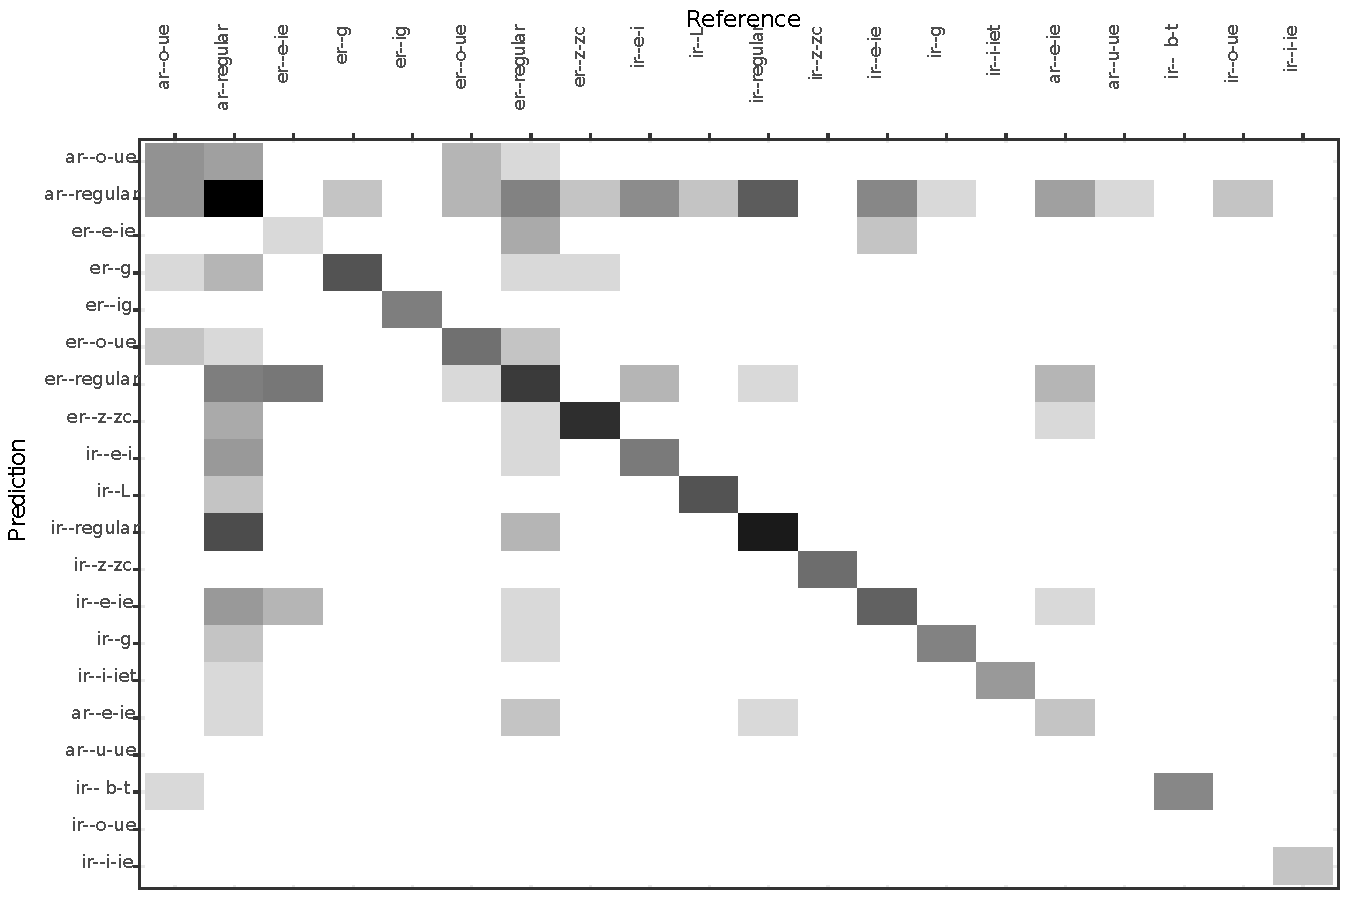
\includegraphics[width=0.85\textheight]{./figures/spanish/p-class-inflection1.pdf}
  \caption{Heat map for the model predicting inflection class of Spanish verbs}
  \label{fig:spanish-verbs-class-v}
\end{sidewaysfigure}


\begin{table}
  \centering
  \scriptsize
  \begin{tabular}{lrrrr}
    \lsptoprule
    \multicolumn{5}{c}{Overall Statistics}                                     \\
    \midrule
    \multicolumn{5}{c}{Accuracy : 0.7772}\\
    \multicolumn{5}{c}{95\% CI : (0.7469, 0.8055)}\\
    \multicolumn{5}{c}{No Information Rate : 0.3329}\\
    \multicolumn{5}{c}{Kappa : 0.7313}\\
    \midrule
    \multicolumn{5}{c}{Statistics by Class:}                                   \\
    \midrule
 &    Class: ar--e$\sim$ie& Class: ar--non-alt& Class: er--e$\sim$ie &Class: er--g\\

    Sensitivity      &             0.2500&             0.7695&          0.0588 &      0.9355\\
    Specificity      &             0.9975&             0.8794&          0.9924 &      0.9961\\
    Neg Pred Value   &             0.9888&             0.8843&          0.9800 &      0.9974\\
    Balanced Accuracy&             0.6237&             0.8245&          0.5256 &      0.9658\\

 &   Class: er--ig &Class: er--o$\sim$ue& Class: er--non-alt &Class: er--z$\sim$zc\\

    Sensitivity        &          1.0000 &         0.6818&             0.7595 &         0.9589\\
    Specificity        &          1.0000 &         0.9924&             0.9561 &         0.9918\\
    Neg Pred Value     &          1.0000 &         0.9911&             0.9735 &         0.9959\\
    Balanced Accuracy  &          1.0000 &         0.8371&             0.8578 &         0.9754\\

 &    Class: ir--e$\sim$i &Class: ir--e$\sim$ie& Class: ir--g &Class: ir--i$\sim$iet\\

    Sensitivity       &            0.4348 &         0.6562&       0.9091 &          1.0000\\
    Specificity       &            0.9898 &         0.9910&       0.9912 &          0.9975\\
    Neg Pred Value    &            0.9835 &         0.9859&       0.9987 &          1.0000\\
    Balanced Accuracy &            0.7123 &         0.8236&       0.9502 &          0.9988\\

 & Class: ir--L &Class: ir--non-alt& Class: ir--z$\sim$zc& Class: ar--o$\sim$ue\\

    Sensitivity         &       0.9355 &            0.8462&          1.0000&          0.5000\\
    Specificity         &       0.9974 &            0.9639&          0.9987&          0.9899\\
    Neg Pred Value      &       0.9974 &            0.9668&          1.0000&          0.9886\\
    Balanced Accuracy   &       0.9665 &            0.9050&          0.9994&          0.7449\\

 &Class: ir--b$\sim$t& Class: ir--i$\sim$ie& Class: ir--o$\sim$ue& Class: ar--u$\sim$ue\\

    Sensitivity          &         1.0000&          0.5000&          0.0000&          0.0000\\
    Specificity          &         0.9987&          1.0000&          1.0000&          1.0000\\
    Neg Pred Value       &         1.0000&          0.9988&          0.9975&          0.9988\\
    Balanced Accuracy    &         0.9994&          0.7500&          0.5000&          0.5000\\
    \lspbottomrule
\end{tabular}
  \caption{Overall and by class statistics for \figref{fig:spanish-verbs-class-v}}
  \label{tab:spanish-verbs-class-v-stats}
\end{table}

These results show that \textit{ar-non-alternating} is still the class with lowest negative predictive value, which means it is the default class for our model, as predicted. Most of the other classes are relatively more or less predictable, with some diphthongization classes having little predictability, like \textit{ir--o$\sim$ue} and \textit{ar--u$\sim$ue}. These are, however, extremely infrequent, with 2 and 1 frequency counts, respectively. It is not surprising that such low-frequency classes should be hard or impossible to predict. It is also expected that combining both dimensions causes some classes to have low predictability. After all, we use the same three predictors to predict sixteen classes, instead of the three and eight from before. The validation results of this final model are presented in \figref{fig:overall-sp-verbs}.% and \figref{fig:byclass-sp-verbs}.

\begin{figure}
  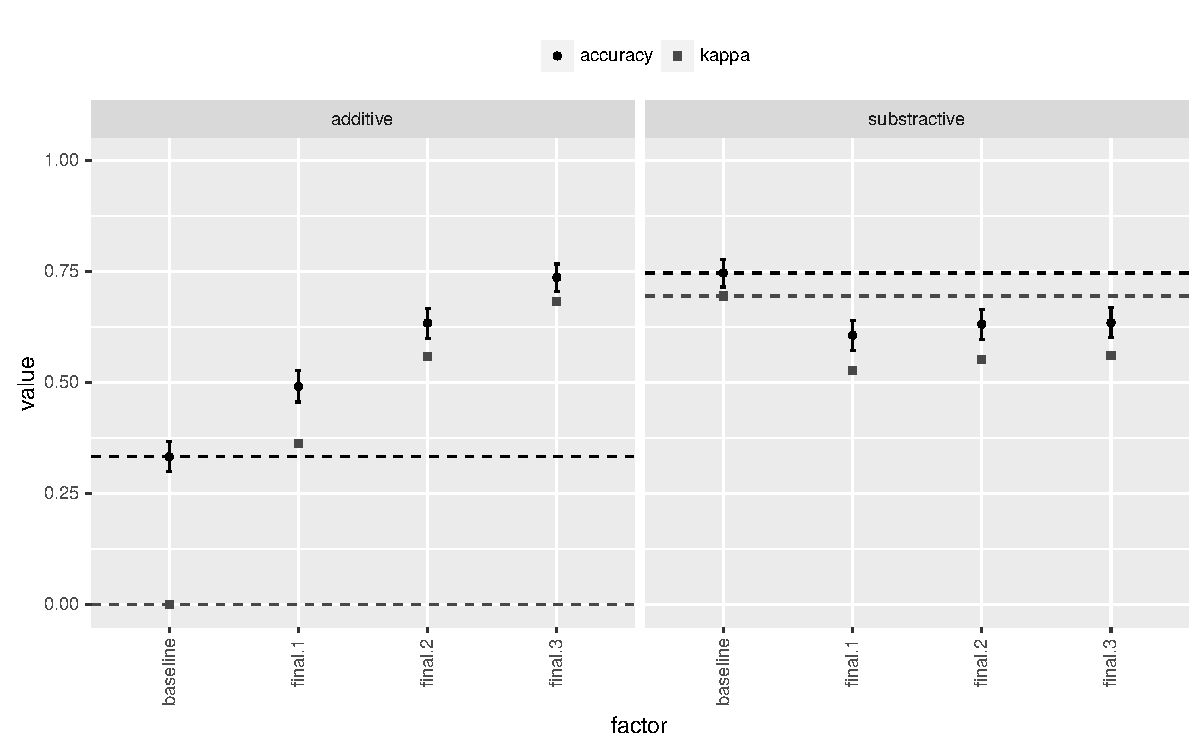
\includegraphics[width=0.9\textwidth]{./figures/spanish/p-fi-mini-overall.pdf}
  \caption{Overall validation  for the model predicting inflection class of Spanish verbs}
  \label{fig:overall-sp-verbs}
\end{figure}

% \begin{sidewaysfigure}
%   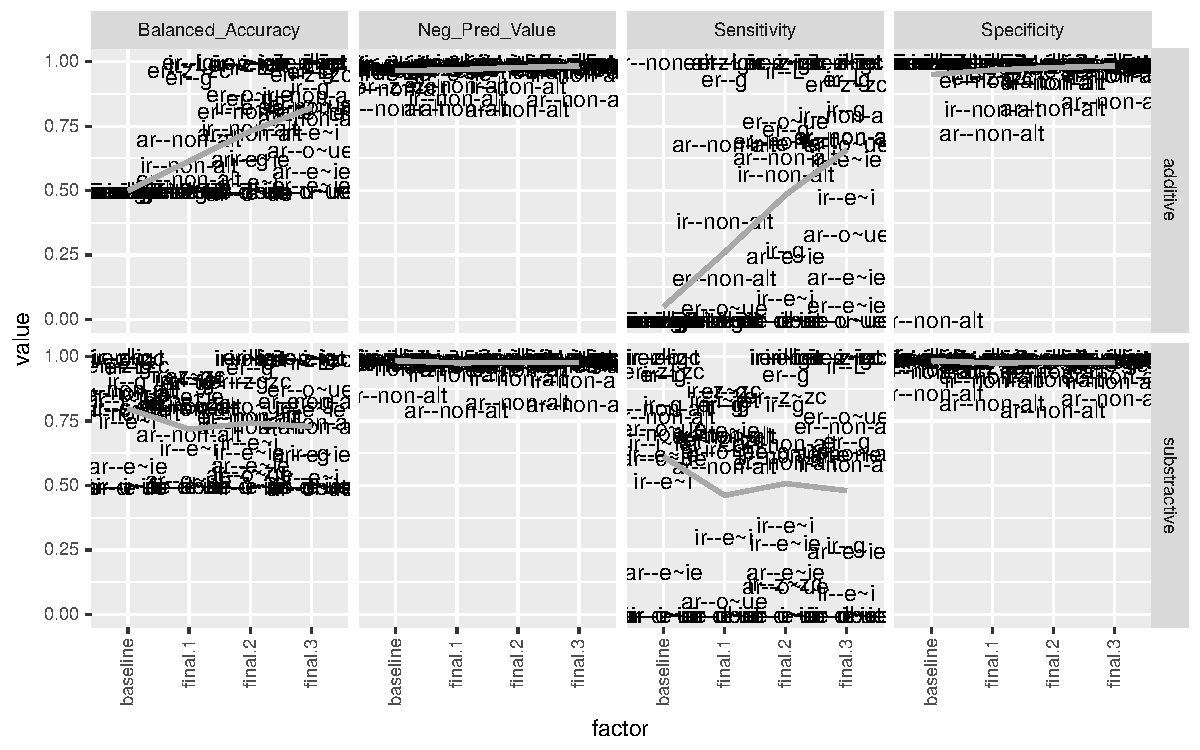
\includegraphics[width=0.9\textheight]{./figures/spanish/p-fi-mini-byclass.pdf}
%   \caption{By class validation  for the model predicting inflection class of Spanish verbs.}
%   \label{fig:byclass-sp-verbs}
% \end{sidewaysfigure}

The results of the MDS and clustering are shown in \figref{fig:sp-fanny-infl}. These clusters exhibit several interesting properties. First, the types \textit{ar--non-alternating}, \textit{er--non-alternating}, and \textit{ir--non-alternating} are all three in the corners of the space. These are maximally different from each other. The color clustering seems less insightful in this case than the MDS, but some groups do form nicely. The least insightful cluster is probably the lila one in the lower left quadrant with the patterns \textit{ir--b$\sim$t} and \textit{ir--z$\sim$zc}, and directly besides this one (in light orange) the alternations \textit{er--ig} and \textit{ir--L}. These two clusters do not seem to follow any pattern, but then again, there is little organization to them. In red we have a clear cluster of \textit{ir--g} and \textit{er--g}, and in dark blue we see a similar situation with the cluster \textit{ar--o$\sim$ue} and \textit{er--o$\sim$ue}. These two clusters organize according to the stem patterns, and not according to the thematic vowels. The class \textit{ir--o$\sim$ue} is very close in the plane to the other two \textit{o$\sim$ue} patterns, but by the hierarchical clustering analysis grouped together with the \textit{ir} alternations \textit{ir--i$\sim$ie} and \textit{ir--i$\sim$iet}. In this case the thematic vowel seems to be more important for the organization of these three patterns. In light blue we have the classes \textit{ir--a$\sim$ie}, \textit{ir--e$\sim$i} and \textit{ir--e$\sim$ie}. Here we see again three classes that basically cluster around stem patterns.

\largerpage 
The clusters are by no means perfect, but they do match the proposed hierarchy to some extent: there are three major inflection patterns that correspond to the thematic vowel, and there are some minor conjugation patterns that cross-classify with these.

\begin{figure}
  \centering
  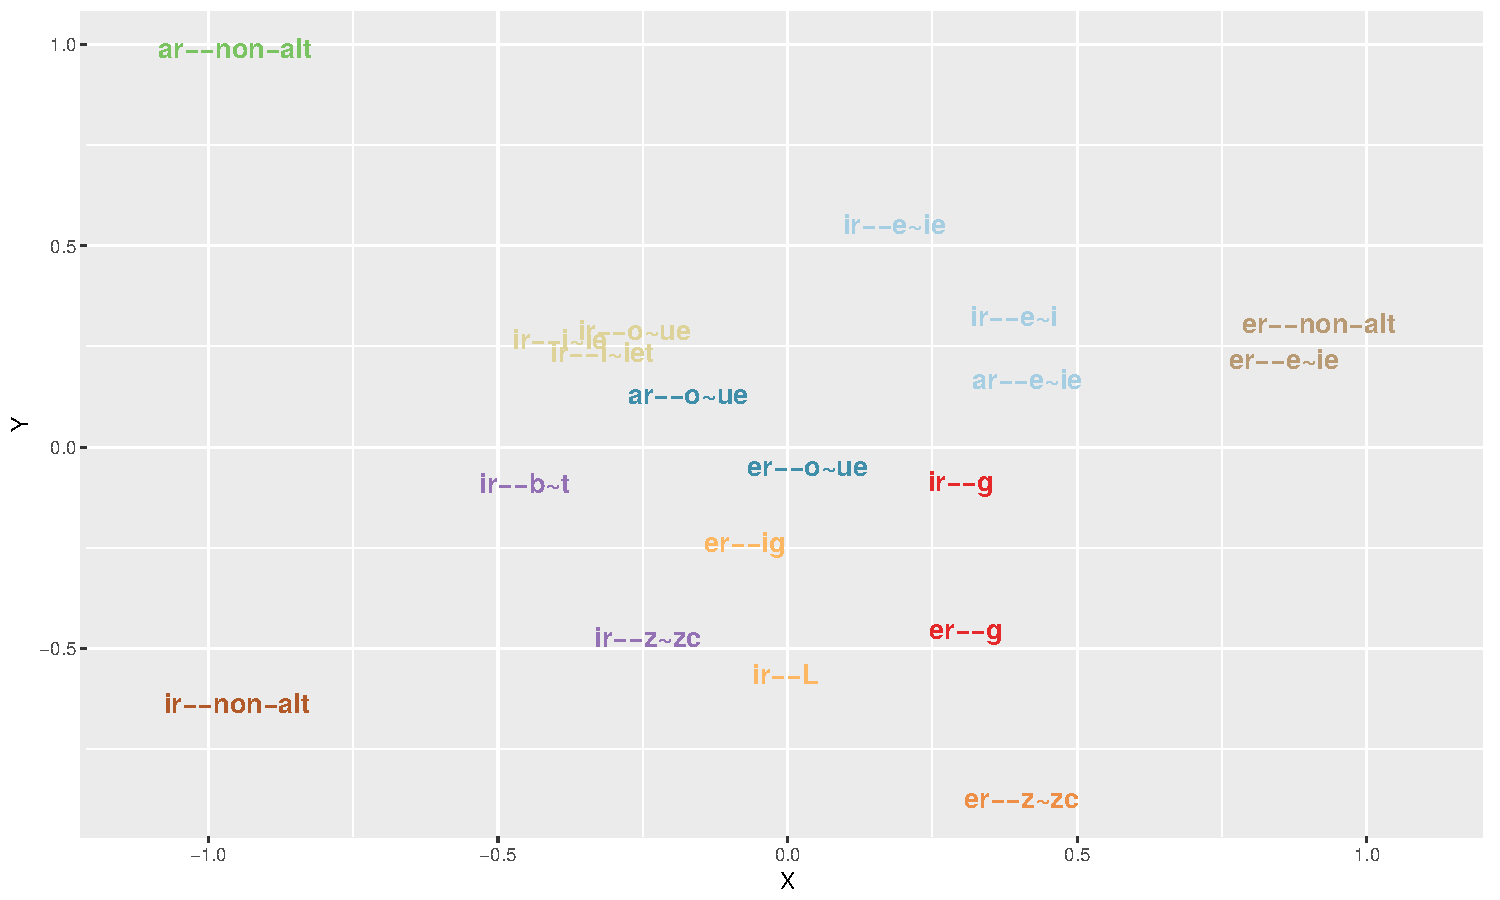
\includegraphics[scale=0.68, angle=90]{./figures/spanish/spanish-verbs-clust-sim1.pdf}
  \caption{Multidimensional scaling with hierarchical clustering for label colors}\label{fig:sp-fanny-infl}
\end{figure}

Some of these effects seem to contradict the claim by \textcite{Albright.2009} that analogical effects are local to the three major classes. These results show that analogical effects between minor patterns run across these three main classes. Although there is no clear explanation for why some clusters prefer to form around the thematic vowel, while others group around the stem patterns, it seems clear that there must be analogical relations that run through both subtrees of the inflection hierarchy of Spanish verbs. In the model I propose here, all dimensions of the hierarchy can carry some analogical information. However, which dimensions will matter most, or where  the strongest similarities will be found, cannot be determined by any particular property of the hierarchy.

For Spanish, it is also interesting to compare the model to the experimental results of \textcite{Albright.2009} mentioned above. As already described, in the original experiment, \textcite{Albright.2001} tested 96 native Spanish speakers on wugs to see whether these wugs would be prone to diphthongization or not. The author used 33 wugs with forms like \textit{lerrar}. Speakers were presented with the verb used in a non-alternating context, like the first person plural (\textit{lerramos}), and then asked to fill in a dialog were the wug appeared in non-alternating and alternating contexts. The authors then calculated the probability of a wug diphthongizing as: the number of speakers who produced a diphthongized form for said wug, over the total number of speakers.

Since we are now predicting experimental data, we can use the complete dataset (with 3000 verbs) without doing any splitting. As the experimental dataset only contains information about mid vowel diphthongs, we have to fit a model trained to predict only this factor. In this case, the previous formula for fitting the model did not perform as well. A more structurally defined model did a much better job: \texttt{diphthong $\sim$ final.1 + final.2 + pre-theme vowel * theme vowel + n\_clusters}\footnote{Because we are now predicting probabilities, using the \texttt{linout} linking function produces better results. The model had no hidden nodes and only a skip layer.}.

This model also takes the final and prefinal segments of the stem, but additionally identifies the pre-thematic vowel interacting with thematic vowel, and the number of consonant clusters\footnote{I take any two consonants appearing together to be a consonant cluster.}. The reason for also adding the thematic vowel is simple. Albright presents a model trained exclusively on \textit{ar} verbs. Adding the thematic vowel in this case means that the model knows what the main portion of the dataset it should look at is when making the predictions, but also has the rest of the dataset to learn from. This is important because our model is less capable of making large phonological generalizations than Albright's is, and every bit of data matters.

When predicting the wugs, the model achieved a correlation of $r=0.59$ ($p<0.05$), which is quite close to the generalized context model \textcite{Albright.2009} reports on ($r=0.56$). It is, however, considerably below the minimal generalization learner ($r=0.77$). The predicted probabilities in \figref{fig:corr-plot} show where the problem lies. The analogical model has difficulties with some wugs ending in complex clusters. This is because these particular combinations are either not present in the data (\textit{etC} is missing) or very rare (\textit{otr} has a frequency of 1). This shows that the generalizations the model makes are too local, and not general enough to capture weird looking wugs correctly. Nevertheless, this is not a bad performance in the sense that the model seems to have some sort of correlate with speaker's intuitions, particularly regarding wugs that do look like observed words. Those cases where speakers were much less likely to allow for diphthongs are also completely disallowed by the model.

\begin{figure}
  \centering
  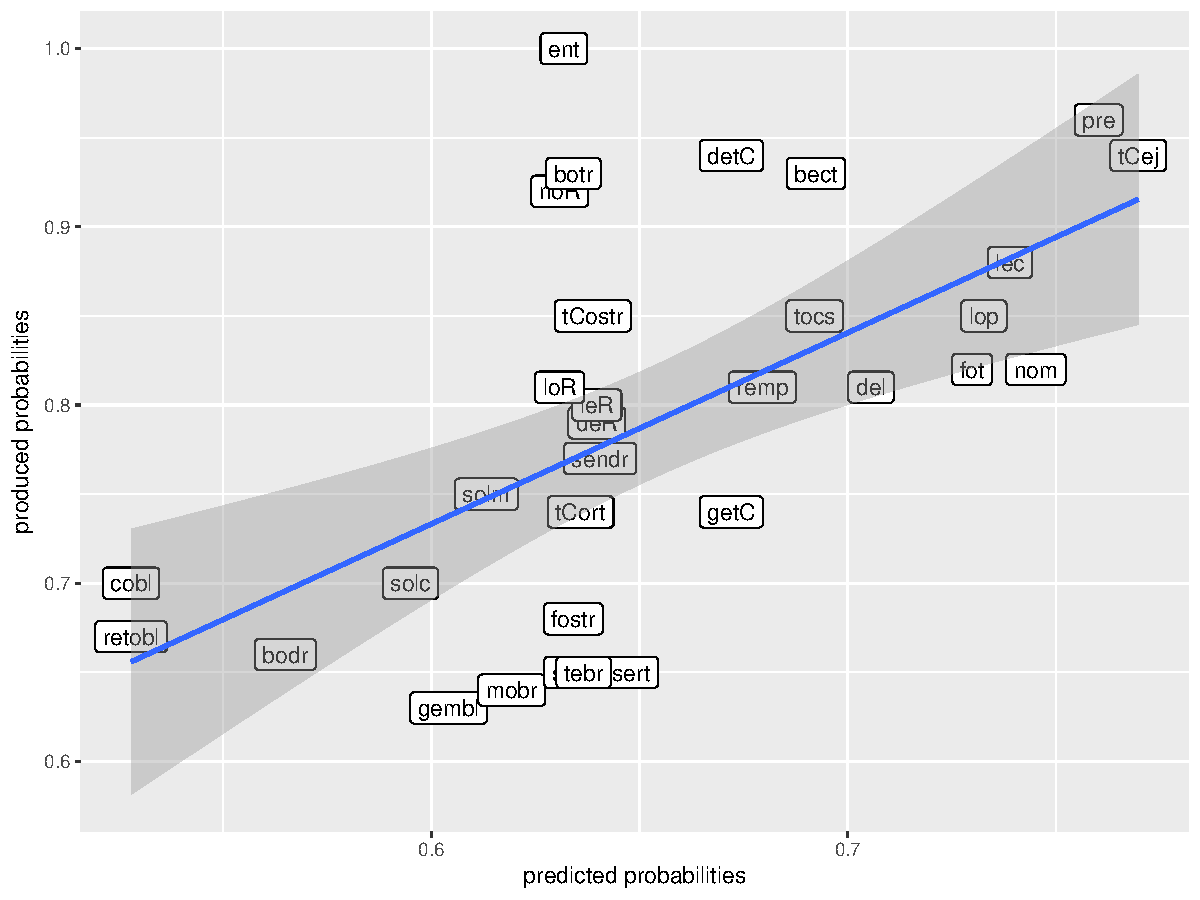
\includegraphics[scale=0.6]{./figures/spanish/corr-plot.pdf}
  \caption{Predicted vs. observed probabilities of diphthong stems}\label{fig:corr-plot}
\end{figure}

The fact that the minimal generalization learner outperforms the analogical model means that the latter is a rougher approximation to what speakers actually do than the former. It is likely that the analogical model better captures the regularities of the synchronic system, but fails to distinguish between truly productive patterns and unproductive patterns. On the other hand, a big downside of Albright's approach is that it only predicts one categorical distinction. In contrast, our model is capable of precise class assignment. Ultimately a more sophisticated system would be required to be able to perform both tasks well: simulate speaker's performance and fine class predictions. Finally, wugs ending in \textit{otr} all get different empirical probabilities. This shows that the initial models that only consider the last three segments are missing something.

\il{Spanish|)}

\section{Cross-classifications between plural and singular: Kasem}

\il{Kasem|(}

Kasem is a Gur Language, of the Grusi branch, spoken mostly in Ghana and Burkina Faso \autocite{Naden.1988}. Kasem featured prominently during the seventies and eighties in phonological debates \autocites{Phelps.1975, Phelps.1979, Halle.1978, deHaas.1987, deHaas.1988} because of coalescence phenomena (see also \citealt{Zaleska.forth.}). Like other Gur languages \autocite{Naden.1989}, Kasem exhibits a complex system of genders and classes that has received relatively little attention in the literature (see \textcite{Awedoba.2003} for some recent discussion of the Kasem gender system, and \textcite{Niggli.2016} for an electronic dictionary of Kasem). Kasem is traditionally analyzed as having 5 genders and 9 nominal classes:

\begin{quotation}
a class is considered singular if the majority of its members are singular, semantically and grammatically; and plural if the majority of its membership is grammatically and semantically plural. There are four singular classes and five plural classes. A pairing of a singular and a plural class constitutes a gender \autocite[4]{Awedoba.2003}
\end{quotation}

Gender is defined with relation to the agreement of the noun with the determiner (most adjectives do not agree at all, and those which do have inherent markers). \textcite[3]{Awedoba.2003} proposes the  classification shown in \tabref{tab:gender-class-kasem} (adapted from the original, and with additional information from \citealt{Awedoba.1980} and \citealt{Awedoba.1996})\footnote{Other sources label the genders with letters from A to E \autocite{Callow.1965}.}. I will show in the following sections that this approach is insufficient to properly capture the complexity of the Kasem system. Nonetheless, the organization in \tabref{tab:gender-class-kasem} already gives us an idea of what the problem is (for work on the noun class systems of related languages see \citealt{Brindle.2009}, \citealt{Bodomo.1994}, \citealt{Bodomo.1997}, and \citealt{Dakubu.1997}): there are five genders based on agreement patterns with pronouns\footnote{The literature does not present any clear examples, but it is mentioned.}, and many more number markers that do not correspond 1 to 1 with said genders. In a way, this is a similar situation to the Romanian system discussed in Chapter \ref{chap:gender-assignment}.

\begin{table}[!htb]
  \centering
  \begin{tabular}{lllllll}
    \lsptoprule
    Gender & \multicolumn{3}{c}{sg. classes} & \multicolumn{3}{c}{pl. classes}           \\

    \midrule
      & noun class & marker  & Det & noun class & marker & Det \\
    1 & I          & u, i, a & wʊm & II         & a      & bam \\
    2 & III        & i       & dɩm & IV         & a      & yam \\
    3 & V          & a       & kam & VI         & i      & sɩm \\
    4 & VII        & u       & kʊm & VIII       & 0, du  & tɩm \\
    5 & VII        & u       & kʊm & IX         & 0, ni  & dɩm \\
    \lspbottomrule
  \end{tabular}\caption{Gender and classes in Kasem}\label{tab:gender-class-kasem}
\end{table}

\textcite[249]{Awedoba.1980} admits that the markers in \tabref{tab:gender-class-kasem} are only the ones he considers to be the most frequent in the language, and that there are other less frequent ones (I will present several additional markers in the following sections). Since the author does not provide an explicit list of all the markers and the genders they define, and because gender assignment is defined by the combination of a noun's singular and plural markers, I will not focus on gender, but rather on the question of how number markers get assigned to nouns\footnote{There is also the more practical problem that the dictionary does not contain gender information. This means that gender can only be infered from the markers themselves.}. This question has been studied before. Some semantic regularities seem to be present in the gender assignment patterns. Gender 1 mostly contains human nouns. Gender 2 contains fruit names and body parts, among others. Gender 3 also contains body parts and names of fruits, but also animals, trees and other plants. Gender 4 seems to be the default class, and Gender 5 is claimed to only contain some 20 nouns mostly related to domestic items. The author concludes that

\begin{quotation}
Kasem Genders are not based on a grouping of homogeneous items. While a gender may contain items from several semantic categories, no gender can be said to monopolise absolutely nouns belonging to any one semantic category \autocite[7]{Awedoba.2003}
\end{quotation}

A further complication for the semantic analysis is that stems can belong to multiple genders. So, while the term for a Kasem person \textit{kasɩnʊ} belongs to Gender 1, the term for the language \textit{kasɩnɩ} belongs to Gender 2. Similarly, diminutives belong to Gender 1, even if the stem belongs to any of the other genders.

Some hints towards the possibility of formal analogical relations are already present, although not spelled out (notice that the author does not tell us what the underlying forms would be in the proposed examples):

\begin{quotation}
  While the semantic bases of the genders cannot be denied, phonology  does also play a role in the allocation of nouns to classes and genders [\dots] The final syllable of a noun, especially the quality of the final vowel, plays some role in the allocation of nouns to their genders. For example, although \textit{bugə} `river', Gender 3 and \textit{bugə} `tiredness', Gender 2 appear to be homophones they are assigned to different classes and genders not necessarily on semantic grounds but perhaps on account of their suffixes, which happen on the surface to be identical but not in deep structure \autocite[12--13]{Awedoba.2003}
\end{quotation}

Similarly, \textcite[250]{Awedoba.1980} had already observed (informally) that gender assignment for loan words in Kasem follows semantic and phonological analogy.

Another important data point mentioned by \textcite[13]{Awedoba.2003} (first found in \cite{Awedoba.1996}), but not discussed with relation to the analogical relations in the system, is the fact that noun-adjective compounds can have different genders independently of the head noun in the compound. So, while \textit{ka-balaŋa} (woman-small, `small woman') belongs to Gender 3, \textit{kə-kəmumu}\footnote{See the following subsection for an explanation on ATR in Kasem.} (woman-big, `big wo\-man') belongs to Gender 4. This indicates that the adjective assigns the gender of the compound, and not the head noun. This is interesting because it means that formal features can easily overcome semantic features in gender assignment in Kasem.

Kasem also has a complex tone system. However, because the dictionary I am relying on \autocite{Niggli.2016} only lists the tones for the singular form, and it is not clear what happens to those tones in many plurals (especially when the number of syllables of the singular and plural are different), I will not consider tone in this study.

\subsection{ATR in Kasem}

In Kasem, as in many West African languages, there is an alternation between [+ATR] (advanced tongue root: /u/, /i/, /ə/, /e/, /o/) and [-ATR] (/ʊ/, /ɩ/, /a/, /ɛ/, /ɔ/) vowels \autocite{Casali.2008}: /ʊ-u/, /ɩ-i/, /a-ə/, /ɛ-e/, /ɔ-o/. Words (with the exception of compounds), have the same [ATR] specification for all their vowels:

\begin{quotation}
In the simplest and most general case of ATR harmony, the vowels in any given word are either all [+ATR] or all [−ATR]. Thus, words in which some vowels are [+ATR] and others [−ATR] do not ordinarily (setting aside certain common classes of exceptions) occur \autocite[496]{Casali.2008}
\end{quotation}

This feature, as can be seen in \REF{atr},\footnote{All Kasem examples are taken from \textcite{Niggli.2016}.} creates minimal pairs and seems to be lexically specified.

\begin{exe}
    \ex \label{atr}
    \begin{tabular}[t]{lllll}
      & singular & plural & gloss                                &   \\
      \midrule
      a. & colo     & cwəəlu & `kilogram'                           & + \\
      b. & cɔlɔ     & cwaalʊ & `girl that likes going out with men' & $-$ \\
      c. & peeli    & peelə  & `shovel, spade'                      & + \\
      d. & pɛɛlɩ    & pɛɛla  & `bean cake'                          & $-$ \\
      f. & vəlu     & vələ   & `traveller'                          & + \\
      e. & valʊ     & vala   & `farmer'                             & $-$ \\
      g. & yiri     & yirə   & `type, kind'                         & + \\
      h. & yɩrɩ     & yɩra   & `name'                               & $-$ \\
    \end{tabular}
\end{exe}

There are, however, some cases in the dictionary where it is not completely clear whether we are dealing with exceptions to this rule or errors in the dictionary itself:

\begin{exe}
    \ex \label{atr-errors}
    \begin{tabular}[t]{llll}
      & singular         & plural          & gloss         \\
      \midrule
      a. & t\textit{a}nti   & t\textit{a}ntiə & `aunt'        \\
      b. & y\textit{u}kwala & yukwalɩ         & `headscarf'   \\
      c. & yukwələ          & yukwəli         & `small skull' \\
    \end{tabular}
\end{exe}

In \REF{atr-errors} there is a supposedly impossible combination of /i/ and /a/, while in the other two examples /u/ appears with both /ə/ and /a/. It is recognized that in ATR harmonizing languages some words may fail to show any harmony, or only present partial harmony \autocite{Casali.2008}, but it is hard to check any of the particular cases in the dictionary.

For Kasem, it is claimed that the [+ATR] feature is carried by the root, and it then extends to the affix \autocite[501]{Casali.2008}. It is mainly for this reason that I will not consider ATR as a predictor or predicted feature of Kasem noun classes. I do not claim that it does not play a role, but counting it in would make an already complex system even more complex.\footnote{In the models I neutralized ATR by converting all [-ATR] vowels to [+ATR].}

\subsection{A simple analysis of Kasem noun classes}

\largerpage
There are different takes on what the number markers in Kasem are. The ones I propose here are based on my own analysis of the system. Alternative models are of course possible, but should have little impact on the analogical system. As a guiding principle for my analysis, I tried to maximize morphology and minimize phonology. Whenever there is enough evidence for a marker to be morphologically motivated, I rejected the phonological explanation for it. This is a conservative approach. In the worst case scenario, I am proposing more markers than there are in the system, which means that the analogical model will have a harder time to predict the classes. A smaller set of markers would result in a better model. %explain why

Kasem has many different number markers, and some of these seem to be more clearcut than others. First, I will introduce the markers where there should be less room for an alternative analysis, and in the following subsection I will introduce those cases where different approaches are possible. This runs counter to the standard way of analyzing Kasem. Previous takes on Kasem have tried to minimize the number of exponents by way of using phonological rules and underlying representations based on some further assumptions. So, for example, \textcite[184]{deHaas.1987} analyses the example in \REF{kasem-wrong-1} as having a marker \textit{-i} which coalesces with the underlying vowel in the stem and turns into /e/, instead of there being a marker \textit{-e}.

\begin{exe}
    \ex \label{kasem-wrong-1}
    \begin{xlist}
        \ex /zwa + i/ $\rightarrow$ /zwe/ `ear'
        \ex /čwa + i/ $\rightarrow$ /čwe/ `liver'
    \end{xlist}
\end{exe}

However, this approach relies on the assumption that \textit{čwe} and \textit{zwe} belong to Gender 2 (Class B in the original) based on the agreement with the determiners, and that all nouns of Gender 2 have a singular marker \textit{-i}. This would make sense if there were compelling evidence from some other morphological process that shows that the stem of these words ends with /a/. In a few cases like \textit{zwe}, one can propose that compounds provide such evidence. The example in \REF{stem-zwe} shows /zwa/ as a stem in three noun-adjective compounds (these are all right-headed compounds, in that order: noun-adjective):

\begin{exe}
    \ex \label{stem-zwe}
    \begin{tabular}[t]{llll}
      & singular  & plural    & gloss             \\
      \midrule
      a. & \textit{zwa}-bɔɔ   & \textit{zwa}-bɔɔrʊ & `hole in the ear' \\
      b. & \textit{zwa}-kɔgɔ  & \textit{zwa}-kwarʊ & `deaf person'     \\
      c. & \textit{zwa}-kwana & \textit{zwa}-kwana & `earring'         \\
    \end{tabular}
\end{exe}

However, there is no such evidence for any of the other 52 nouns that end in /e/ in the singular in the dictionary, and there is even counter evidence for a general rule. In \REF{stem-E-base} we see what could be thought to be examples just as \textit{zwe}, where a noun belongs to Gender 2, takes the singular marker \textit{-i} and the plural marker \textit{-ə}, but because the stem ends in /ə/, the /i/ surfaces as /e/.

\begin{exe}
    \ex \label{stem-E-base}
    \begin{tabular}[t]{llll}
      & singular        & plural                        & gloss         \\
      \midrule
      a. & kalw\textit{e}  & kalw\textit{ə}, kal\textit{i} & `monkey'      \\
      b. & kandw\textit{ɛ} & kandw\textit{a}               & `stone, rock' \\
    \end{tabular}
\end{exe}

However, compounds built from these nouns do seem to have a /ə/ in the stem, as shown in \REF{stem-E-compounds} below.

\begin{exe}
    \ex \label{stem-E-compounds}
    \begin{tabular}[t]{llll}
      & singular      & plural        & gloss                                          \\
      \midrule
      a. & kalw\textit{e}-faa     & kalwe-faarʊ   & `baboon'                                       \\
      b. & kalw\textit{e}-sɩŋa    & kalwe-sɩna    & `Red Patas Monkey'                             \\
      c. & kalw\textit{e}-zwənə   & kalwe-zwəm    & `Green Monkey'                                 \\
      d. & kandw\textit{ɛ}-gara   & kandwa-garɩ   & `dike' \\
      e. & kandw\textit{ɛ}-nyɩɩnɩ & kandwa-nyɩɩna & `bright / shiny stone'                         \\
    \end{tabular}
\end{exe}

What this means is that even if the phonological analysis is right in the case of \textit{zwe}\footnote{Even in this case it is unclear that this is the right analysis. It is not obvious that the form found in the compound is the stem, since the head noun of a compound can show some variation: \textit{tu-mwɛn} `shrub, bush, small tree' in the singular has the form \textit{t\emph{we}-mwan} in the plural.}, we cannot automatically assume that this analysis applies to all nouns ending in /e/. A systematic study of each case would have to be undertaken, but because of the limitations of the dataset I am using, this is not feasible. For this reason, I will take markers to be what they appear to be in their surface form, unless there is clear and strong evidence to the contrary.

\subsubsection{Basic number markers}

An important feature of Kasem is that the same number markers can appear as singular markers in some nouns, and as plural markers in other nouns. The main markers (i.e. the most common ones) are: \textit{-e}, \textit{-ə}, \textit{-i}, \textit{-o}, \textit{-u},  \textit{-nə} and \textit{-nu}. We see in \REF{ipl-kasem} examples of the \textit{-i} marker in the plural, with the \textit{-ə} marker in the singular. In \REF{isg-kasem} we have the inverse situation. In both examples there is an assumption of coalescence between the /i/ in the stem and the /i/ in the marker (/i+i/ $\rightarrow$ /i/). In following sections I will discuss the possibility of an \textit{-iə} marker instead.

\begin{exe}
    \ex \label{ipl-kasem}
    \begin{tabular}[t]{llll}
      & singular        & plural         & gloss        \\
      \midrule
      a. & afɩdɩ\textit{a} & afɩd\textit{ɩ} & `sugar cane' \\
      b. & bordi\textit{ə} & bord\textit{i} & `plantation' \\
    \end{tabular}
\end{exe}

\begin{exe}
    \ex\label{isg-kasem}
    \begin{tabular}[t]{llll}
      & singular       & plural          & gloss        \\
      \midrule
      a. & b\textit{i}    & bi\textit{ə}    & `counter'    \\
      b. & pɔmp\textit{ɩ} & pɔmpɩ\textit{a} & `water pump' \\
    \end{tabular}
\end{exe}

This is not the only possible analysis of these examples. One could also postulate a zero marker for the singular and a \textit{-ə} marker in the plural. In this case the data are not enough to clearly distinguish between all the alternatives. I have tried to always take the most conservative approach.\footnote{For purposes of the models, in these cases the stem was taken to be \textit{pɔmp} or \textit{b}, without an additional \textit{-i}.}

Examples in \REF{esg-kasem} and \REF{epl-kasem} show the alternation between the \textit{-e} marker and the \textit{-ə} marker for both singular and plural.

\begin{exe}
    \ex \label{esg-kasem}
    \begin{tabular}[t]{llll}
      & singular & plural  & gloss             \\
      \midrule
      a. & cicw\textit{e}    & cicw\textit{ə}   & `spear'           \\
      b. & nafʊzw\textit{ɛ}  & nafʊzw\textit{a} & `chapped fingers' \\
    \end{tabular}
\end{exe}

\begin{exe}
    \ex \label{epl-kasem}
    \begin{tabular}[t]{llll}
      & singular & plural & gloss             \\
      \midrule
      a. & gungwəŋ\textit{ə} & gungw\textit{e} & `hour-glass drum' \\
      b. & paya\textit{a}    & pay\textit{ɛ}   & `jaw'             \\
    \end{tabular}
\end{exe}

The examples in \REF{osg-kasem} and \REF{opl-kasem} show the \textit{-o} and \textit{-u} markers. While the \textit{-o} marker rarely appears in the plural (and then only with another \textit{-o} marker in the singular), the \textit{-u} marker can be found both for plural and singular.

\begin{exe}
    \ex \label{osg-kasem}
    \begin{tabular}[t]{llll}
      & singular        & plural                           & gloss                    \\
      \midrule
      a. & bol\textit{o}   & bwəəl\textit{u}, bwəll\textit{u} & `valley, low land'       \\
      b. & tasɔr\textit{ɔ} & taswaar\textit{ʊ}                & `flint lighter, lighter' \\
    \end{tabular}
\end{exe}

\begin{exe}
    \ex \label{opl-kasem}
    \begin{tabular}[t]{llll}
      & singular & plural  & gloss                    \\
      \midrule
      a. & yukol\textit{o}   & yukoll\textit{o} & `skull'                  \\
      b. & yɩrɩn\textit{ʊ}   & yɩrɩn\textit{a}  & `security guard, warden' \\
      c. & tiəb\textit{u}    & tiəbi\textit{ə}  & `cat'                    \\
    \end{tabular}
\end{exe}

Finally, in \REF{nupl-kasem} and \REF{nepl-kasem} we see some examples of the \textit{-nu} and \textit{-nə} markers. Both markers are almost exclusively found in the plural. The marker \textit{-nu} always appears with lengthening of either the vowel or the consonant,
and can only co-occur with either \textit{-ŋɔ} or \textit{-ŋu} in the singular, while the marker \textit{-nə} can appear without lengthening in certain cases and is less restricted in terms of the singular markers it can combine with, although it tends to be pair with \textit{-m}.

\begin{exe}
    \ex \label{nupl-kasem}
    \begin{tabular}[t]{llll}
      & singular & plural  & gloss                           \\
      \midrule
      a. & dɔŋɔ     & daa\textit{nʊ}   & `sticks to support a flat roof' \\
      b. & luluŋu   & lulun\textit{nu} & `perspiration'                  \\
    \end{tabular}
\end{exe}

\begin{exe}
    \ex \label{nepl-kasem}
    \begin{tabular}[t]{llll}
      & singular & plural & gloss        \\
      \midrule
      a. & jazɩm    & jazɩ\textit{na} & `right hand' \\
      b. & zuŋə     & zu\textit{nə}   & `bird'       \\
    \end{tabular}
\end{exe}

These are the simple, straightforward number markers in Kasem. These examples show that the language allows for reversals \autocite{Baerman.2007}, where pairs of markers flip their value depending on the noun. This will be one important point in the analysis.

\subsubsection{The \textit{-ŋ-} and \textit{-g-} markers}

I now turn to less straightforward cases. Many words show a /ŋ/ segment in the singular that does not appear in the plural. Sometimes this segment is the final segment in the word, but it is mostly followed by what appears to be a regular singular marker like those discussed above. For this reason it has been claimed that the /ŋ/ is part of the singular stem, and that it tends to disappear in the plural \autocites{Callow.1965, Awedoba.1980}. Thus, examples like those in  \REF{delete-ng} are analyzed as having an \textit{-ə} marker in the singular and an \textit{-e} marker in the plural. This, however, is no different from claiming that /ŋ/ is a singular marker which alternates with other markers for the plural, with the caveat that it can then somewhat freely combine with additional singular markers. There does not seem to be anything special about these examples that make them different from others.

\begin{exe}
    \ex \label{delete-ng}
    \begin{tabular}[t]{llll}
         & singular             & plural      & gloss                         \\
      \midrule
      a. & wu-sa\textit{ŋa}     & wu-sɛ       & `second flute'                \\
      b. & baya-pwə\textit{ŋə}  & baya-pwəənu & `illness where the eyes,       \\
         &                      &             &  feet and hands are swollen' \\
      c. & bugəni-zu\textit{ŋə} & bugəni-zunə & `stork'                       \\
    \end{tabular}
\end{exe}

It is then worth asking whether we are dealing with two co-occurring markers \textit{-ŋ-} and \textit{-ə} (in a case of multiple exponence), or if there is an additional, independent marker \textit{-ŋə}. Looking more closely it becomes clear that \textit{-ŋ-} can appear with \textit{-ə}, \textit{-o} and \textit{-u}. Some examples are given in \REF{exes-ng}. These examples show that the marker \textit{-ŋV} often alternates with \textit{-nu}, but not necessarily, which is evidence that these are co-occurring markers.

\begin{exe}
    \ex \label{exes-ng}
    \begin{tabular}[t]{llll}
      & singular        & plural    & gloss                       \\
      \midrule
      a. & nyɩ\textit{ŋa}  & nyɩa, nyɩ & `horn'                      \\
      b. & bwə\textit{ŋə}  & bwe       & `adultery'                  \\
      c. & lɔ\textit{ŋɔ}   & lwaanʊ    & `distance, length, surface' \\
      d. & bulo\textit{ŋo} & bulwənnu  & `liana'                     \\
      e. & ku\textit{ŋu}   & kunnu     & `Bohor Reedbook'            \\
      f. & bʊ\textit{ŋʊ}   & bʊnnʊ     & `root'                      \\
    \end{tabular}
\end{exe}

An additional argument against the phonological analysis that states that /ŋ/ is in the stem and gets deleted in the plural can be seen in \REF{except-ng2}, where an apparent  \textit{-ŋV} alternates with a \textit{-ŋa} marker, or an \textit{-i} or \textit{-iə}. Although it is hard to distinguish between both alternatives, /ŋ/ is not simply deleted in the plural.

\begin{exe}
    \ex \label{except-ng2} \textsc{sg} tɩtʊŋɩ \textsc{pl} tɩtʊŋa, tɩtwɩa `work, occupation'
\end{exe}

The existence of the five examples in \REF{except-ng3} makes things more complex, because here \textit{-ŋ} appears as a marker on its own. As we will see later, there is a $\emptyset$ marker in Kasem, which means this could be a case of \textit{-ŋ-$\emptyset$}, but also simply a \textit{-ŋ} final marker.

\begin{exe}
    \ex \label{except-ng3}
    \begin{tabular}[t]{llll}
      & singular        & plural              & gloss                               \\
      \midrule
      a. & do\textit{ŋ}    & donnə               & `mate, fellow, friend'             \\
      b. & bado\textit{ŋ}  & badonnə             & `friend, colleague, comrade'        \\
      c. & cilo\textit{ŋ}  & cilonnə, ciloonə    & `friend'                            \\
      d. & ka-do\textit{ŋ} & ka-donnə            & `fellow wife'                       \\
      e. & yuudo\textit{ŋ} & yuudonnə, yuudwəənə & `mate, friend of same age, \\
      &&& comrade' \\
    \end{tabular}
\end{exe}

A similar marker to the \textit{-ŋ-} marker just discussed, is the \textit{-g-} marker. Like \textit{-ŋ-}, this marker can also only appear with \textit{-ə}, \textit{-o} and \textit{-u}, and it exclusively marks singular. Some examples are given under \REF{g-exe-kasem}.

\begin{exe}
    \ex \label{g-exe-kasem}
    \begin{tabular}[t]{llll}
      & singular & plural    & gloss                         \\
      \midrule
      a. & gar-di\textit{gə} & gar-di    & `mosquito net'                \\
      b. & jɩ\textit{ga}     & jɩɩ, je      & `place, location'          \\
      c. & po\textit{go}     & pwəru     & `spider's web'                \\
      d. & sʊ\textit{gʊ}     & sʊm, sʊnɩ & `knife, razor'                \\
      e. & kaju\textit{gu}   & kajuru    & `head pad for carrying loads' \\
    \end{tabular}
\end{exe}

The distribution of theses \textit{-gV} markers with the corresponding plural markers is also not very restricted, particularly for \textit{-gə}. \textcites{Callow.1965} also claims that this marker is a stem phoneme that undergoes a phonological deletion process.

The claim that \textit{ŋ} and \textit{g} are part of the stem is not well argued for in the literature. One argument in favour of this kind of analysis seems to be based on evidence from compounds like those in \REF{ng-deletion}. The assumption is that singular markers cannot appear inside compounds.

\begin{exe}
    \ex \label{ng-deletion}
    \begin{tabular}[t]{llll}
      & singular & plural & gloss \\
      \midrule
      a. & zʊŋa     & zunə   & `bowl, calabash'       \\
      b. & zʊŋ-biə  & zʊŋ-bi & `calabash used for measuring'        \\
      c. & zʊŋ-diə  & zʊŋ-di & `calabash for eating food, eating bowl'        \\
    \end{tabular}
\end{exe}

This kind of evidence is rather weak and not very systematic, however. For example, in cases like those in \REF{no-g-deletion}, the /g/ segment does not appear in the compounds of the noun, so one could just as well say that based on this evidence, \textit{-g-} has to be a marker.

\begin{exe}
    \ex \label{no-g-deletion}
    \begin{tabular}[t]{llll}
         & singular & plural & gloss                                \\
      \midrule
      a. & digə     & di     & `hut, room, house'                   \\
      b. & di-niə   & di-ni  & `married woman's principal room'     \\
      c. & di-yuu   & di-yum & `woman's annex room,                  \\
         &          &        &  inner kitchen in the rainy season' \\
    \end{tabular}
\end{exe}

Similarly, some compounds use the complete singular form of the noun, like those in \REF{ng-in-compound}.

\begin{exe}
    \ex \label{ng-in-compound}
    \begin{tabular}[t]{llll}
      & singular    & plural      & gloss           \\
      \midrule
      a. & sɔŋɔ        & swannʊ      & `shea-nut tree' \\
      b. & sɔŋɔ-sabara & sɔŋɔ-sabarɩ & `tree species'  \\
    \end{tabular}
\end{exe}

Thus, evidence from compounds to infer stems is contradictory.

Finally, whether we should consider \textit{-ŋ-} and \textit{-g-} as independent markers or postulate at least six \textit{-}[\textit{+velar}]\textit{V} markers seems to be a secondary issue. As a middle ground, I posit a  system where \textit{-ŋ-} and \textit{-g-} can combine with other singular markers, while being markers on their own. Unlike the \textit{-ə}, \textit{-o} and \textit{-u} markers \textit{-ŋ-} and \textit{-g-} can combine with, \textit{-ŋ-} and \textit{-g-} are (almost) exclusively singular markers. In the end, however, this will not make any difference for the analogical models.

\subsubsection{The \textit{-r-} marker}

\largerpage[2]
A similar situation arises in the plural with the \textit{-rV}\footnote{In earlier works it is common to find a reference to a marker \textit{du} instead. This seems to be because /r/ and /d/ are allophones in the language. Since the source I am using uses /r/, I will use this notation.} markers. The examples in \REF{rupl-kasem} show the \textit{-r-} marker, which almost exclusively appears in the plural (with the exception of the two words in \REF{rusg-kasem-2}). We find \textit{-r-} appearing mostly with \textit{-ə} and \textit{u}, and only in a few cases with \textit{-o}. Additionally, the \textit{-ru} combination is found co-occurring with quite a few different singular markers.

\begin{exe}
    \ex \label{rupl-kasem}
    \begin{tabular}[t]{llll}
      & singular  & plural     & gloss                      \\
      \midrule
      a. & ba-dʊ\textit{gʊ}   & ba-dʊ\textit{rʊ}    & `sterile man'              \\
      b. & cibu-po\textit{go} & cibu-pwə\textit{ru} & `chick of about one month' \\
      c. & du\textit{du}      & duduu\textit{rə}    & `musical instrument'       \\
      d. & tabu\textit{lo}    & taabulo\textit{ro}  & `black board'              \\
    \end{tabular}
\end{exe}

The example in \REF{rusg-kasem-2} shows that there are at least two apparent exceptions where \textit{-ru} appears in the singular. It is hard to know how to interpret these cases. It could be that in fact \textit{-r-} can appear in the singular but is dispreferred, or it could be that these are special cases that require some different kind of analysis.

\begin{exe}
    \ex \label{rusg-kasem-2}
    \begin{tabular}[t]{llll}
      & singular & plural    & gloss              \\
      \midrule
      a. & ba\textit{rʊ}     & banna     & `husband, partner' \\
      b. & kan-ba\textit{rʊ} & kan-banna & `husband'          \\
    \end{tabular}
\end{exe}

\subsubsection{The \textit{-m} marker}

\largerpage 
A particularly hard case is found in the \textit{-Vm}/\textit{-nV} pairs, like those shown in \REF{nm-exe}.

\begin{exe}
    \ex \label{nm-exe}
    \begin{tabular}[t]{llll}
      & singular  & plural     & gloss                  \\
      \midrule
      a. & badə\textit{m}     & badənə     & `bachelor'             \\
      b. & banɩ-nyɩ\textit{m} & banɩ-nyɩna & `disrespectful person' \\
      c. & dʊ\textit{m}       & dʊna       & `enemy'                \\
    \end{tabular}
\end{exe}

There are several possible analyses for these examples. The more phonological one would suggest a sort of coalescence process between an /m/ segment of the stem and the \textit{-nV} marker. Alternatively, one could argue that the fact that the sequence /mV/ is not found in singular forms suggests that the vowel is turning the /m/ into an /n/, and the fact that the final vowel of the singular is often kept in the plural strongly suggests that the stem ends in /m/, and these are examples of nouns without a singular marker. There are, however, several facts that speak against a phonological explanation. First of all, pairs like these can be found for the plural (with lower frequency, however):

\begin{exe}
    \ex \textsc{sg} baloja\textit{na} \textsc{pl} baleja\textit{m} `Buzzard'
\end{exe}

If these were a purely phonological process, the symmetry would be a bit suspicious. Particularly, cases like those in \REF{except-m} are more in line with an \textit{-m} marker, rather than an /m/ stem and coalescence.

\begin{exe}
    \ex \label{except-m}
    \begin{tabular}[t]{llll}
      & singular & plural  & gloss                          \\
      \midrule
      a. & bɛɛs\textit{ɩm}   & bɛɛs\textit{a}   & `torment, torture, oppression' \\
      b. & kadag\textit{um}  & kadag\textit{wi} & `kind of sorghum'              \\
    \end{tabular}
\end{exe}


Although one could postulate some kind of /m/ deletion rule, this overly complicates what could be a straightforward system. This is even more clear from the perspective of the plural, especially cases with overabundance as those shown in \REF{over-m}.

\begin{exe}
    \ex \label{over-m}
    \begin{tabular}[t]{llll}
         & singular & plural             & gloss                              \\
      \midrule
      a. & di-yuu   & di-yum             & `woman's annex room,               \\
         &          &                    & inner kitchen in the rainy season' \\
      b. & ga-sugu  & ga-sum             & `wild Guinea fowl'                 \\
      c. & sɔŋɔ     & \textit{sam, sanɩ} & `house, compound'                  \\
      d. & sugu     & \textit{sum, suni} & `guinea-fowl'                      \\
      e. & sʊgʊ     & \textit{sʊm, sʊnɩ} & `knife, razor, cutlass'            \\
    \end{tabular}
\end{exe}

These examples are strong evidence that this is not a phonological process, but rather a morphological one. I will thus consider \textit{-m} to be a marker in its own right.

\subsubsection{The \textit{-iə} marker}

This particular marker is even harder to argue for, particularly in the light of the \textit{-ə} marker (discussed above). For most cases, it is not completely clear whether we are dealing with a \textit{-iə}/\textit{-i} class, or with a \textit{-ə}/\textit{-0} class, where either the plural or singular is expressed by a zero marker. In \REF{ia-kazem} we see a couple of examples:

\begin{exe}
    \ex \label{ia-kazem}
    \begin{tabular}[t]{llll}
      & singular & plural   & gloss                          \\
      \midrule
      a. & manjɩs\textit{ɩ}  & manjɩs\textit{ɩa} & `matches'                      \\
      b. & mɩam\textit{ɩa}   & mɩam\textit{ɩ}    & `imported body creams/lotions' \\
    \end{tabular}
\end{exe}

This is especially difficult in cases where the opposing marker is an \textit{-e}, since one could just as well postulate a phonological rule which reduces /ie/ into /e/.

\begin{exe}
    \ex \label{ia2-kazem}
    \begin{tabular}[t]{llll}
      & singular  & plural   & gloss             \\
      \midrule
      a. & kwər-dɩa  & kwər-dɛ  & `loud voice'      \\
      b. & kunku-bɩa & kunku-bɛ & `soldier termite' \\
    \end{tabular}
\end{exe}

For both examples either analysis would work. The only clear evidence we have for an \textit{-iə} marker comes from a few examples where nouns have a /iə/ in the plural and something else in the singular, or where we get a clearly different plural marker:

\begin{exe}
    \ex
    \begin{tabular}[t]{llll}
      & singular  & plural           & gloss                       \\
      \midrule
      a. & dɩndwɛ    & dɩndwɩa          & `dream'                     \\
      b. & ga-digəbu & ga-digəbiə       & `African wild cat'          \\
      c. & kabəl-bu  & kabəl-biə        & `small soup-bowl for sauce' \\
      d. & naniə    & nan\textit{iinə} & `cow'                       \\
    \end{tabular}
\end{exe}

I will assume an \textit{-iə} marker, but acknowledge that there are many cases were it is not completely straightforward, from the dictionary alone, to determine whether we are actually dealing with a \textit{-iə} marker or a \textit{-ə} marker.

\subsubsection{The \textit{-n} marker}

Some examples like those in \REF{n-kazem} show for both singular and plural what appears to be an \textit{-n} marker.

\begin{exe}
    \ex \label{n-kazem}
    \begin{tabular}[t]{llll}
      & singular   & plural     & gloss                               \\
      \midrule
      a. & bugə-nyʊan & bugə-nywɩn & `plant'                             \\
      b. & gwiən      & gwin       & `Yellow-billed Shrike'              \\
      c. & bʊcwɛn     & bʊcwan     & `goat that has not yet given birth' \\
      d. & bu-kwɩʊn   & bu-kwɩɩrʊ  & `adolescent'                        \\
      e. & baŋa       & bɛn        & `bracelet, bangle, metal ring'      \\
    \end{tabular}
\end{exe}

In this case one could, as before, postulate and additional series of \textit{-Vn} markers, or a \textit{-n} marker which can co-occur with other singular and plural markers. Since there does not appear to be evidence that could distinguish between either hypothesis, I will assume that this is again a case of multiple exponence, but the alternative should not have any impact on the implementation of the model.

\subsubsection{Three minor markers: the \textit{-iine}, \textit{-si} and $\emptyset$ markers}

The final two segmental markers are the marker \textit{-iine}, shown in \REF{inne-kasem}, and the \textit{-si} marker in \REF{si-kasem}.

\begin{exe}
    \ex \label{inne-kasem}
    \begin{tabular}[t]{llll}
      & singular & plural    & gloss              \\
      \midrule
      a. & bar-nu   & bar-n\textit{iinə}  & `mother-in-law'    \\
      b. & fitə-tu  & fitə-t\textit{iinə} & `mechanic, fitter' \\
    \end{tabular}
\end{exe}

\begin{exe}
    \ex \label{si-kasem}
    \begin{tabular}[t]{llll}
      & singular  & plural     & gloss           \\
      \midrule
      a. & dʊ-baga   & dʊ-bag\textit{sɩ}   & `thunder'       \\
      b. & ga-cawaka & ga-cawag\textit{sɩ} & `shrub species' \\
    \end{tabular}
\end{exe}

These two markers are infrequent and are not featured in the literature, but it seems unlikely that they could be analyzed as resulting from phonological processes.

Finally, there is a $\emptyset$ marker. This marker is rather rare, with only 15 examples, 12 of which end in /[+velar]ə/ in the singular. Of course, a \textit{no marker} alternative works equally well and makes no real difference for the analysis. A phonological explanation could work for those cases where there is a final vowel (like in (\ref{0-kasem}d)), in which one could postulate coalescence between the vowel in the stem and the marker, and thus we do not see any extra marker. But this explanation is much less likely for the examples with a consonant ending.

\begin{exe}
    \ex \label{0-kasem}
    \begin{tabular}[t]{llll}
      & singular          & plural           & gloss                \\
      \midrule
      a. & kɔn               & kɔɔn\textit{a}   & `Roan Antelope, Kob' \\
      b. & kwan              & kwan             & `water-lily'         \\
      c. & plan              & plaan\textit{rʊ} & `plan, map'          \\
      d. & mancɩ\textit{ga}  & mancɩ            & `manioc, cassava'    \\
      e. & gar-di\textit{gə} & gar-di           & `mosquito net'       \\
      f. & bancɩ\textit{ga}  & bancɩ            & `manioc, cassava'    \\
    \end{tabular}
\end{exe}

In these examples it is clear that forms like \textit{mancɩ} or \textit{bancɩ} have no plural marker because the singular contains them entirely, and adds some additional marker which does not otherwise combine, or follow a vocalic marker (i.e. \textit{-gə} does not follow an \textit{-ɩ} marker).

\subsubsection{Lengthening and diphthongization}\label{sec:lengthening}

There are two phonological processes found in Kasem which seem to mark plurality in addition to the individual segmental markers presented before. These are: lengthening of the stem and diphthongization of the last vowel of the stem.

\begin{exe}
    \ex \label{dp-kasem1}
    \begin{tabular}[t]{llll}
      & singular & plural & gloss                          \\
      \midrule
      a. & logo & lwəru    & `hole dug for planting seed, seed-hole' \\
      b. & ŋwɩʊ & ŋwɩɩrʊ   & `wage, payment'                         \\
      c. & pulu & pullu    & `granary made of straw'                 \\
    \end{tabular}
\end{exe}

In (\ref{dp-kasem1}b) we see that the lengthening can be of the last vowel and in (\ref{dp-kasem1}c) we see that it can be of the last consonant. This strongly speaks for a mora insertion which can either attach to the consonant or vowel. This analysis is supported by some overabundant examples where both effects are found. In \REF{CCVV-kasem} we see that this phenomenon is even independent of the additional segmental plural marker chosen.

\begin{exe}
    \ex \label{CCVV-kasem}
    \begin{tabular}[t]{llll}
      & singular  & plural     & gloss           \\
      \midrule
      a.& cʊrʊ& cʊrrʊ, cʊʊrʊ& `black make-up'\\
      b.& vɔrɔ& vannɩ, vaanʊ& `hoe'\\
    \end{tabular}
\end{exe}

Especially interesting are the cases where both processes (i.e. lengthening and diphthongization) occur on the same word as shown in \REF{Ldp-kasem}.

\begin{exe}
    \ex \label{Ldp-kasem}
    \begin{tabular}[t]{llll}
         & singular     & plural         & gloss                        \\
      \midrule
      a. & bugə-kanyɔnɔ & bugə-kanywannʊ & `kind of tree'               \\
      b. & yolo         & ywəllu         & `empty area / field,         \\
         &              &                & empty space outside village' \\
      c. & cɔlɔ         & cwaalʊ         & `girl that likes going out   \\
         &              &                & with men'                    \\
      d. & war-boro     & war-bwəəru     & `brick mould / mold'         \\
    \end{tabular}
\end{exe}

\subsubsection{Other stem changes}

Some nouns show some sort of unpredictable stem changes, mostly in velar segments as seen in \REF{other-kasem-1}

\begin{exe}
    \ex \label{other-kasem-1}
    \begin{tabular}[t]{llll}
      & singular & plural       & gloss               \\
      \midrule
      a. & coro     & ceeni, ceenu & `hen, fowl, chicken' \\
      b. & boŋo     & bənnu        & `dung, shit'        \\
      c. & biboku   & bibəgəru     & `stutterer'         \\
      d. & cɩkʊ     & cɩgɩrʊ       & `trap'              \\
      e. & cɩcʊgʊ   & cɩkʊrʊ       & `feather of fowls'  \\
    \end{tabular}
\end{exe}

I do not consider suppletion among the classes for the analogical model, but in principle this could also be a dimension of noun inflection.

\subsubsection{Compounds}

\largerpage
For most compounds, the only part that changes is the rightmost (the adjective). There are, however, exceptions with compounds with the word \textit{kandwɛ} `stone', among some others as in \REF{except-stone}.

\begin{exe}
    \ex \label{except-stone}
    \begin{tabular}[t]{llll}
         & singular       & plural                   & gloss                          \\
      \midrule
      a. & kandwɛ-nyɩɩnɩ  & kandw\textit{a}-nyɩɩna   & `bright / shiny stone'         \\
      b. & kandwɛ-ŋʊnɩ    & kandw\textit{a}-ŋʊna     & `precious / bright stone,       \\
         &                &                          & jewels, pearl.'              \\
      c. & kandwɛ-pɩsɩɩnɩ & kandw\textit{a}-pɩsɩɩna  & `pile / heap of stones'        \\
      d. & kandwɛ-pʊlɔrɔ  & kandw\textit{a}-palwaarʊ & `rock'                         \\
      e. & kandwɛ-pʊpʊrʊ  & kandw\textit{a}-pʊpʊrrʊ  & `stone bracelet'               \\
      f. & kunkwən-poŋo   & kunkwə\textit{ŋ}-pwəənu  & `Red-eyed Dove,\\
      &&&  collared dove' \\
    \end{tabular}
\end{exe}

I will leave this case as an open problem since the data are not conclusive as to why some compounds can inflect for their head noun and others do not.

\subsection{Materials}

The dataset, as well as all examples cited here, come from the Kasem Burkina Faso Dictionary \autocite{Niggli.2016} in its online version.\footnote{\url{http://kassem-bf.webonary.org/}, visited on 10-11-2016.} The dictionary lists for each noun its singular and plural forms, as well as the tones for the singular form. The tones for the plural form are only listed in a few exceptional cases, which seems to suggest that the plural and singular forms have the same tones. This, however, is hard to extrapolate to words where the plural is longer or shorter than the singular. From 2000 nouns listed in the dictionary, I removed 30 cases where either the marker was completely unclear, the plural showed unpredictable suppletion, or where there was reason to suspect an error (i.e. nouns where the ATR feature did not match across all their vowels, etc.), and ended up with a total of 1970 nouns.

For the two nouns in \REF{kasem-alt-sing} the dictionary presented an alternative in the singular. For both these cases I only considered the main form.

\begin{exe}
    \ex \label{kasem-alt-sing}
    \begin{xlist}
        \ex kwɩan (kwɛ)  `Stripped Ground Squirrel'
        \ex sɛ (swɛ)  `ivory bracelet'
    \end{xlist}
\end{exe}

In the cases of polysemy I left all entries in the table:

\begin{exe}
    \ex \label{kasem-syn}
    \begin{xlist}
        \ex ni `opening of a room/house, gate'
        \ex ni `mouth, beak'
        \ex \dots
    \end{xlist}
\end{exe}

\largerpage[2]
As we have seen in multiple examples already, Kasem, just like Hausa, presents some overabundance in the plural forms:

\begin{exe}
    \ex \label{kasem-over-pl}
    \begin{tabular}[t]{llll}
      & singular & plural      & gloss      \\
      \midrule
      a. & bwana    & bwanɩ, bwam & `mosquito' \\
      b. & bʊŋʊ     & bʊnɩ, bʊm   & `goat'     \\
    \end{tabular}
\end{exe}

In all these cases I only considered the first plural listed. The reason is that the dictionary only lists 108 nouns with overabundant plurals. This is not enough to be able to reliably model overabundance in this case.

For roughly half of the nouns, the dictionary included a semantic annotation which consists of some basic groupings like `animal', `human', `animate', etc., coded with numbers. I use this semantic annotation in the analogical models. As for the nouns without semantic coding, I assigned them to a default class.

\subsection{Modelling the system}

After the previous discussion it is useful to look at the pairings between segmental singular and plural markers. \tabref{tab:comarkers-kasem} shows the number of nouns for which a given pairing holds (ignoring overabundant cases), after neutralizing ATR. The table also ignores lengthening and diphthongization. \tabref{tab:coplural-kasem} shows the co-occurrences of plural markers with either lengthening of the vowel (VV), the consonant (CC), and with the presence or absence of diphthongization.

\begin{sidewaystable}
    \centering
    \small
    \begin{tabular}{rrrrrrrrrrrrrrrrrrrrrr}
      \lsptoprule
      & \multicolumn{19}{c}{Plural}\\
      \midrule
      Singular & 0  & e  & ə   & en & ən & i   & iə & iinə & in & m  & n & ne & nə & ni & nu & o & rə & ro & ru & si & u   \\
      \midrule
      0  & 2  & 0  & 3   & 0  & 0  & 0   & 0  & 0    & 0  & 0  & 0 & 0  & 0  & 0  & 0  & 0 & 0  & 0  & 1  & 0  & 0   \\
      e  & 0  & 1  & 48  & 0  & 0  & 0   & 2  & 0    & 0  & 0  & 0 & 0  & 0  & 0  & 0  & 0 & 0  & 0  & 1  & 0  & 0   \\
      ə  & 3  & 28 & 33  & 0  & 0  & 236 & 0  & 0    & 0  & 0  & 0 & 0  & 2  & 2  & 0  & 0 & 0  & 0  & 41 & 10 & 2   \\
      en & 0  & 0  & 1   & 0  & 8  & 0   & 0  & 0    & 0  & 0  & 0 & 0  & 0  & 0  & 0  & 0 & 0  & 0  & 0  & 0  & 0   \\
      ən & 0  & 1  & 0   & 0  & 1  & 0   & 0  & 0    & 7  & 0  & 1 & 0  & 0  & 0  & 0  & 0 & 0  & 0  & 3  & 0  & 0   \\
      gə & 19 & 20 & 1   & 0  & 0  & 17  & 0  & 0    & 0  & 0  & 0 & 1  & 0  & 0  & 0  & 0 & 1  & 0  & 2  & 1  & 0   \\
      go & 0  & 0  & 0   & 0  & 0  & 0   & 0  & 0    & 0  & 0  & 0 & 0  & 0  & 0  & 1  & 0 & 0  & 2  & 53 & 0  & 0   \\
      gu & 0  & 0  & 0   & 0  & 0  & 0   & 0  & 0    & 0  & 3  & 0 & 0  & 0  & 0  & 0  & 0 & 0  & 0  & 34 & 0  & 0   \\
      i  & 0  & 0  & 321 & 0  & 0  & 9   & 27 & 0    & 0  & 0  & 0 & 0  & 1  & 0  & 0  & 0 & 0  & 0  & 1  & 0  & 0   \\
      iə & 0  & 14 & 0   & 0  & 0  & 32  & 4  & 3    & 1  & 0  & 0 & 0  & 1  & 2  & 0  & 0 & 3  & 0  & 1  & 2  & 0   \\
      in & 0  & 0  & 0   & 0  & 0  & 0   & 1  & 0    & 0  & 0  & 0 & 0  & 0  & 0  & 0  & 0 & 0  & 0  & 1  & 0  & 0   \\
      m  & 0  & 0  & 12  & 0  & 0  & 1   & 0  & 0    & 0  & 1  & 0 & 0  & 64 & 0  & 0  & 0 & 0  & 0  & 0  & 0  & 0   \\
      nə & 0  & 0  & 0   & 0  & 0  & 0   & 0  & 0    & 0  & 24 & 0 & 0  & 0  & 0  & 0  & 0 & 0  & 0  & 0  & 0  & 0   \\
      ŋ  & 0  & 0  & 0   & 0  & 0  & 0   & 0  & 0    & 0  & 0  & 0 & 0  & 5  & 0  & 0  & 0 & 0  & 0  & 0  & 0  & 0   \\
      ŋə & 8  & 42 & 1   & 9  & 0  & 9   & 0  & 0    & 9  & 0  & 1 & 0  & 7  & 0  & 2  & 0 & 0  & 0  & 0  & 1  & 0   \\
      ŋi & 0  & 0  & 1   & 0  & 0  & 0   & 0  & 0    & 0  & 0  & 0 & 0  & 0  & 0  & 0  & 0 & 0  & 0  & 0  & 0  & 0   \\
      ŋo & 1  & 0  & 0   & 0  & 0  & 0   & 0  & 0    & 0  & 1  & 0 & 0  & 3  & 0  & 91 & 0 & 0  & 0  & 0  & 0  & 0   \\
      ŋu & 0  & 0  & 0   & 0  & 0  & 0   & 0  & 0    & 0  & 0  & 0 & 0  & 1  & 1  & 35 & 0 & 0  & 0  & 0  & 0  & 0   \\
      no & 0  & 0  & 0   & 0  & 0  & 0   & 0  & 0    & 0  & 0  & 0 & 0  & 0  & 0  & 0  & 0 & 0  & 0  & 1  & 0  & 0   \\
      o  & 0  & 0  & 11  & 0  & 0  & 0   & 0  & 0    & 0  & 0  & 0 & 0  & 0  & 6  & 0  & 5 & 0  & 1  & 42 & 0  & 137 \\
      on & 0  & 0  & 0   & 0  & 0  & 0   & 0  & 0    & 0  & 0  & 0 & 0  & 0  & 0  & 0  & 0 & 0  & 0  & 2  & 0  & 0   \\
      ru & 0  & 0  & 0   & 0  & 0  & 0   & 0  & 0    & 0  & 0  & 0 & 0  & 2  & 0  & 0  & 0 & 0  & 0  & 0  & 0  & 0   \\
      u  & 1  & 1  & 160 & 0  & 0  & 0   & 40 & 12   & 0  & 1  & 0 & 0  & 2  & 4  & 0  & 0 & 1  & 0  & 75 & 0  & 78  \\
      un & 0  & 0  & 0   & 0  & 0  & 0   & 0  & 0    & 0  & 0  & 0 & 0  & 0  & 0  & 0  & 0 & 0  & 0  & 4  & 0  & 0   \\
      \lspbottomrule
    \end{tabular}
    \caption{Co-occurrence of singular and plural markers}\label{tab:comarkers-kasem}
\end{sidewaystable}

\begin{sidewaystable}
    \small
    \begin{tabular}{rr@{\hspace{1.5\tabcolsep}}r@{\hspace{1.5\tabcolsep}}r@{\hspace{1.5\tabcolsep}}r@{\hspace{1.5\tabcolsep}}r@{\hspace{1.5\tabcolsep}}r@{\hspace{1.5\tabcolsep}}r@{\hspace{1.5\tabcolsep}}r@{\hspace{1.5\tabcolsep}}r@{\hspace{1.5\tabcolsep}}r@{\hspace{1.5\tabcolsep}}r@{\hspace{1.5\tabcolsep}}r@{\hspace{1.5\tabcolsep}}r@{\hspace{1.5\tabcolsep}}r@{\hspace{1.5\tabcolsep}}r@{\hspace{1.5\tabcolsep}}r@{\hspace{1.5\tabcolsep}}r@{\hspace{1.5\tabcolsep}}r@{\hspace{1.5\tabcolsep}}r@{\hspace{1.5\tabcolsep}}r@{\hspace{1.5\tabcolsep}}r}
      \lsptoprule
      & \multicolumn{19}{c}{Plural marker}\\
      \midrule
      & 0  & e   & ə   & en & ən & i   & iə & iinə & in & m  & n & ne & nə & ni & nu & o & rə & ro & ru  & si & u   \\
      \midrule
      no-lengthening   & 32 & 106 & 411 & 9  & 9  & 297 & 73 & 0    & 17 & 30 & 2 & 1  & 74 & 4  & 0  & 0 & 4  & 2  & 107 & 14 & 8   \\
      CC-lengthening   & 0  & 0   & 6   & 0  & 0  & 0   & 0  & 0    & 0  & 0  & 0 & 0  & 8  & 1  & 48 & 5 & 0  & 0  & 1   & 0  & 72  \\
      VV-lengthening & 2  & 1   & 175 & 0  & 0  & 7   & 1  & 15   & 0  & 0  & 0 & 0  & 6  & 10 & 81 & 0 & 1  & 1  & 154 & 0  & 137 \\
      \midrule
      no-diphthongization  & 33 & 101 & 565 & 9  & 9  & 277 & 74 & 15   & 17 & 29 & 2 & 1  & 84 & 15 & 39 & 5 & 5  & 3  & 192 & 14 & 83  \\
      diphthongization     & 1  & 6   & 27  & 0  & 0  & 27  & 0  & 0    & 0  & 1  & 0 & 0  & 4  & 0  & 90 & 0 & 0  & 0  & 70  & 0  & 134 \\
      \lspbottomrule
    \end{tabular}
    \caption{Co-occurrence of plural markers with lengthening and diphthongization}\label{tab:coplural-kasem}
\end{sidewaystable}

\begin{table}[!htbp]
  \centering
  \begin{tabular}{lrr}
    \lsptoprule
    &diphthongization  &no-diphthongization\\
    \midrule
    CC-lengthening     &24  &117\\
    no-lengthening    &108 &1092\\
    VV-lengthening    &228  &362\\
    \lspbottomrule
  \end{tabular}\caption{Co-occurrence of lengthening and diphthongization}
  \label{tab:codp-length-kasem}
\end{table}

If we cross-classify all factors the result are 144 nonempty classes (ignoring ATR), with most classes having less than 50 members, and 63 classes of only 1 member. Because of this, a flat list of inflection classes looks particularly unconvincing. A more straightforward approach is to use cross-classification as with the Spanish systems.

\largerpage[2]
To model the complete space of inflectional classes several trees are required. The first thing we have to recognize is that markers like \textit{-i}, are not in themselves plural or singular markers, but simply number markers. Whether they indicate plural or singular depends on their distribution with other markers. There are two alternatives at this point, either overspecification as in \figref{fig:number-markers-kasem}, or underspecification as in \figref{fig:number-markers-kasem-under}.

\begin{figure}
    \caption{Kasem number markers with overspecification}\label{fig:number-markers-kasem} 
    \begin{forest} baseline, 
      for tree={parent anchor=south, align=center, child anchor=north}
        [\textit{number}
        [\textit{singular}, name=SG [-g-] [-ŋ-] [-e, name=E] [-ə, name=SHW] [-i, name=I]]
        [\textit{plural}, name=PL [$\emptyset$, name=NULL] [-o, name=O] [-u, name=U] [-si] [-iine]]]
        \draw (E.north) -- (PL.south);
        \draw (SHW.north) -- (PL.south);
        \draw (I.north) -- (PL.south);
        \draw (NULL.north) -- (SG.south);
        \draw (O.north) -- (SG.south);
        \draw (U.north) -- (SG.south);
    \end{forest}
\end{figure}

\begin{figure}
    \caption{Kasem number markers with overspecification} \label{fig:number-markers-kasem-under}  
    \begin{forest} baseline, 
      for tree={parent anchor=south, align=center, child anchor=north}
        [\textit{number}
        [\textit{singular}, name=SG [-g-] [-ŋ-]]
        [-e, name=E] [-ə, name=SHW] [-i, name=I]
        [$\emptyset$, name=NULL] [-o, name=O] [-u, name=U]
        [\textit{plural}, name=PL  [-si] [-iine]]]
    \end{forest}
\end{figure}

\newpage 
For the purposes of this study either alternative would work equally well. For simplicity I will go with the underspecification approach in \figref{fig:number-markers-kasem-under}. 

Lengthening and diphthongization are processes which are completely independent of the segmental markers, but from \tabref{tab:coplural-kasem} it should be clear that the distribution of plural markers is not random with regards to the classes they co-occur with. Both are much more likely with \textit{-u} markers, and lengthening of the vowel is also very likely with \textit{-ə}. Similarly, we see that while \textit{-ru} is very likely to co-occur with lengthening of the vowel, it only co-occurs once with lengthening of the consonant, as shown in \REF{length-ru-cc}.

\begin{exe}
    \ex \label{length-ru-cc} \textsc{sg} ŋwam-pʊgʊ \textsc{pl} ŋwam-pʊrrʊ `scale of wound'
\end{exe}

Similarly, as can be seen in \tabref{tab:codp-length-kasem}, the proportion of words with no lengthening in the plural but diphthongization is around 10\%, while that of CC-lenth\-ening and diphthongization is around 20\%, and the proportion of nouns with diphthongization and VV-lengthening is of almost 40\%. These are clearly not random distributions\footnote{I skip statistical tests here because I will show this is the case with the models in the next section.}. What this means is that our model for cross-inheritance should consider all four factors: segmental markers of the singular, segmental markers of the plural, lengthening and diphthongization.

Because lengthening and diphthongization only occur on the stem, these two dimensions can also be modelled with a stem space. For this, we have to postulate that Kasem nouns have a singular and a plural stem. Alternatively, nonconcatenative morphological processes could also be used to account for these changes. In the end, the important thing is that all nouns must be specified for whether they undergo these processes or not. The partial trees for lengthening and diphthongization can be trivially defined as in \figref{fig:length-tree-kasem} and \figref{fig:diph-tree-kasem}.

\begin{figure}
    \caption{Hierarchy for lengthening in Kasem} \label{fig:length-tree-kasem}
    \begin{forest} baseline, 
      for tree={parent anchor=south, align=center, child anchor=north}
        [\textit{lengthening}
        [\textit{no-length}]
        [\textit{length} [\textit{vowel}] [\textit{consonant}]]]
    \end{forest}
\end{figure}

\begin{figure}
    \caption{Hierarchy for dipthongization in Kasem} \label{fig:diph-tree-kasem}
    \begin{forest}baseline, 
      for tree={parent anchor=south, align=center, child anchor=north}
        [\textit{diphthongization} [\textit{no-diphthong}, name=NODIPH] [\textit{diphthong}, name=DIPH]]
    \end{forest}
\end{figure}

\figref{fig:partial-kasem} shows a partial hierarchy with all dimensions of Kasem noun inflection class. Segmental markers constitute a hierarchy of their own, which specifies which markers combine with which other markers. Underspecified markers can mark either singular or plural, and the combination of two of these underspecified markers means that both alternatives are available\footnote{It is however unclear if for all combinations of underspecified markers reversals are found. In other words, if \textit{x} and \textit{y} are underspecified, it is not clear whether \textit{x-y} and \textit{y-x} necessarily exist, or that it could exist.}. The complete inflection class of a noun is given by the \textit{sg-pl--diphth--length}.

\begin{sidewaysfigure}
  \centering
  \scalebox{0.7}{\begin{forest} %qtree, 
      for tree={parent anchor=south, align=center, child anchor=north}
    [\textit{number-class}, for tree={parent anchor=south, child anchor=north}
    [\textit{segmental-markers}
    [\textit{singular}
    [\textit{-ŋ-} [\textit{-ŋu}, name=ŋu][\textit{-ŋә}, name=ŋә]]
    [\textit{-g}- [\textit{-gu}, name=gu] [\textit{-gә}, name=gә, [\textit{gә-ә}, tier=cl2, name=gәә]]]
    ]
    [\textit{underspecified}
    [\textit{-e}, name=e [\textit{e-ә}, name=eә]]
    [\textit{-i}, name=i [\textit{i-ә}, name=iә] [\textit{i-i}]]
    [\textit{-ә}, name=ә [\textit{ә-e}, name=әe] [\textit{ә-ә}, name=әә]]
    %[$\emptyset$, name=E]
    [\textit{-n}, name=n [\textit{-en}, name=en] [\textit{-әn}, name=әn]]
    [$\emptyset$, name=E]
    [\textit{-u}, name=u]
    ]
    [\textit{plural} 
    %[\textit{-si}] 
    %[\textit{-iine}]
    [\textit{-r-} [\textit{-ru}, name=ru,
    [$\emptyset$\textit{-ru}, name=emptyru]] [\textit{-rә}, name=rә]]
    [\textit{-si}] 
    [\textit{-iine}]
    ]]
    [\textit{stem}
    [\textit{length} [\textit{no-length}, name=nl, tier=cl2 [\textit{i-ә--ndiphth--nl}, name=iәnd
    [alapɩl `aeroplane'\\ ankɩt `handkerchief']]]
    [\textit{length} [\textit{vv}, tier=cl2] [\textit{cc}, tier=cl2]]]
    [\textit{diphthong} [\textit{no-diphth}, tier=cl2, name=ndp] [\textit{diphth}, tier=cl2
    [\textit{gә-ә--diphth--nl}, name=gәәdp
    [jafʊ `fingernail']]
    [\textit{ә-ә--diphth--nl}, name=әәdp
    [nʊ `calf' \\ sisu `young guinea fowl']]]]]]
    \draw (en.north) -- (e.south);
    \draw (әn.north) -- (ә.south);
    \draw (rә.north) -- (ә.south);
    \draw (ru.north) -- (u.south);
    \draw (eә.north) -- (ә.south);
    \draw (әe.north) -- (e.south);
    \draw (emptyru.north) -- (E.south);
    \draw (әәdp.north) -- (ә.south);
    \draw (әәdp.north) -- (nl.south);
    \draw (gәә.north) -- (ә.south);
    \draw (gәәdp.north) -- (gәә.south);
    \draw (gәәdp.north) -- (nl.south);
    \draw (iә.north) -- (ә.south);
    \draw (iәnd.north) -- (ndp.south);
    \draw (iәnd.north) -- (iә.south);
  \end{forest}}
  \caption{Partial inflection class hierarchy for Kasem}\label{fig:partial-kasem}
\end{sidewaysfigure}

Every noun in Kasem must be typed for its complete inflection class. In \figref{fig:partial-kasem} the lexeme \textit{alapɩl} `aeroplane' belongs to class \textit{i-ә--ndiphth--nl}, which means it takes an \textit{i} in the singular, a \textit{ә} in the plural, and its stem does not undergo diphthongization or lengthening. How different theories chose to realize these properties, is an independent problem.

\subsection{Methodological considerations}

\subsubsection{Predictability between subtrees}

In several of the models below, when predicting a subtree (e.g. \textit{lengthening}), I will include information from another subtree (e.g. \textit{diphthongization}). From a theoretical perspective, this works in a different way than the stem information. Adding information about a cross-classifying tree is equivalent to removing a subset of the possible classes. In the toy example in \figref{fig:exe-cross-model-info}, two subtress, $\tau$ and $\sigma$, cross-classify to build the inflection classes for the lexemes \textit{w}$_1$ to \textit{w}$_9$. If an analogical model predicting $\tau$ for the words \textit{w}$_1$ to \textit{w}$_9$, knows $\sigma$, it will not have to decide between three classes, but at most two. For words \textit{w}$_7$ to \textit{w}$_9$, the type \textit{s2} uniquely determines that these words belong to type \textit{t3}, because it removes the possibility that these words could belong to either \textit{t1} or \textit{t2}. For words \textit{w}$_1$ to \textit{w}$_6$, the type \textit{s1} removes the possibility of \textit{t3}.

\begin{figure}
    \caption{Example of cross-classifications and information} \label{fig:exe-cross-model-info} 
    \begin{forest} baseline
        [\textit{class}, for tree={parent anchor=south, child anchor=north}
        [$\tau$,tier=cl1 [\textit{t1}, name=t1 [\textit{w}$_1$] [\textit{w}$_2$] [\textit{w}$_3$]]
        [\textit{t2}, name=t2 [\textit{w}$_4$] [\textit{w}$_5$] [\textit{w}$_6$]] [\textit{t3}, name=t3 [\textit{w}$_7$] [\textit{w}$_8$] [\textit{w}$_9$]]]
        [$\sigma$ [\textit{s1}, name=s1, tier=cl1] [\textit{s2}, name=s2, tier=cl1]]]
        \draw (s1.south) -- (t1.north);
        \draw (s1.south) -- (t2.north);
        \draw (s2.south) -- (t3.north);
    \end{forest}
\end{figure}

\subsubsection{Compounds}

We now turn to the analogical modelling. A difficult decision regarding this particular dataset is whether to include compounds or not. Including them means that, because compounds usually have the same plural marker as the simplex noun, the model will be able to remember some cases. That is, the cross-validation is not completely perfect. On the other hand, not all compounds share the same plural marker as their simplex form. Additionally, it is not always clear what sort of compounds we are actually dealing with. Some seem semantically transparent like those in (\ref{different-pl-kasem}a) and (\ref{different-pl-kasem}b), but others less so like those in (\ref{different-pl-kasem}f) and (\ref{different-pl-kasem}g).

\begin{exe}
    \ex \label{different-pl-kasem}
    \begin{tabular}[t]{llll}
      & singular                         & plural     & gloss                          \\
      \midrule
      a. & baŋa       & bɛn        & `bracelet, bangle, metal ring' \\
      b. & kalɩm-baŋa & kalɩm-bɛ   & `black bracelet (for rites)'   \\
      c. & nyasaŋ-biə                       & nyasaŋ-biə & `sesame seeds'    \\
      d. & zʊŋ-biə                          & zʊŋ-bi     & `calabash used for measuring'\\
      e. & bʊŋʊ                             & bʊnɩ, bʊm  & `goat'  \\
      f. & bʊŋʊ       & bʊnnʊ      & `root'                         \\
      g. & ŋwan-bʊŋʊ  & ŋwan-bʊnnʊ & `capillary'                    \\
    \end{tabular}
\end{exe}

Finally, not all words marked as compounds in the dictionary have a corresponding simplex form:

\begin{exe}
    \ex \label{no-simplex-kasem}
    \begin{tabular}[t]{ll@{}lll}
         &   & singular   & plural     & gloss          \\
      \midrule
      a. &   & kaləŋ-jarʊ & kaləŋ-jara & `fisherman'    \\
      b. &   & wo-jaanʊ   & wo-jaana   & `bird, insect' \\
      c. &   & kamɔ-mɔrʊ  & kamɔ-mɔra  & `potter'       \\
      d. & * & jarʊ                                    \\
      e. & * & jaanʊ                                   \\
      f. & * & mɔrʊ                                    \\
    \end{tabular}
\end{exe}

There are only around 200 nouns which appear multiple times because they are present as simplex forms and compounds. One could still remove them from the dataset, considering the examples in \REF{different-pl-kasem} and \REF{no-simplex-kasem}, we see that compounds do not guarantee consistent plural endings, and do not guarantee a simplex forms. With this in mind, leaving the compounds in is not much too different from having items where the last three or four segments are identical. We would not remove these cases, since these are the core of what the analogical process is. Similarly, that compounds tend to belong to the same class as the simplex form, seems to also be a product of the same principles. Finally, from a more cognitive perspective, the fact that there are many lexical entries with the same stem simply means that there are more chances to memorize that form. In any case, it seems more realistic to leave the compounds in.

\subsection{Results}

The dataset extracted from the dictionary had 1970 nouns. Considering all these nouns, the total number of classes (disregarding lengthening and diphthongization) was 98, with 48 classes having one or two members. Although possible in theory, in practical terms it is very difficult to fit and evaluated models with this kind of distribution. On the one hand, it is impractical because there are just not enough training data for most classes, and on the other hand, errors in the very low frequency classes will unfairly penalize the model's performance. For this reason I removed all items that belong to a class with a type frequency of 8 or less. The final dataset contains a total of 1792 nouns, distributed across 33 classes. This leaves us with a system that has more classes than any of the other examples discussed in this book.

The predictors are: the last three segments of the singular stem (computed as the singular without the singular marker), the semantic annotation in the dictionary, the lengthening process (C lengthening, V lengthening, or none), the diphthongization process (none or present), the singular marker and the plural marker. As mentioned above, because ATR is a stem feature, I neutralized it for all stems. The length (in letters) of the stem and the tones of the singular form did not play any role in the models.

Because of its complexity, I will present several different models that tackle different parts of the system. The following sections describe the results for each such model. I will only look at clustering of the results for the last model predicting inflectional class. There are many more possible combinations I did not test, but the most important aspects of the system are covered.

\subsubsection{Predicting diphthongization}\label{subsec:pred-diph}

The first case we look at is diphthongization in the plural. Since it is a binary choice, this is the simplest of the models for Kasem. The basic model (not including number markers) was: \texttt{diphthong $\sim$ final.1 + final.2 + final.3 + meaning}\footnote{For all Kasem models the networks only included a skip layer and no hidden layers, with a decay rate of 0.01.}. \tabref{tab:diph-kasem-1} presents the results with  the corresponding accuracy scores in \tabref{tab:diph-kasem-1-stats}.

\begin{table}
  \centering
  \begin{tabular}{lrr}
    \lsptoprule
    &Reference\\
    \midrule
    Prediction & dp  & Ndp  \\
    dp         & 267 & 66   \\
    Ndp        & 79  & 1380 \\
    \lspbottomrule
  \end{tabular}
  \caption{Confusion matrix for the model predicting diphthongization without segmental number markers in Kasem}
  \label{tab:diph-kasem-1}
\end{table}

\begin{table}
  \centering
  \begin{tabular}{rl}
    \lsptoprule
    \multicolumn{2}{c}{Overall Statistics}   \\
    \midrule
    Accuracy :            & 0.9191           \\
    95\% CI :             & (0.9055, 0.9313) \\
    No Information Rate : & 0.8069           \\
    Kappa :               & 0.7366           \\
    \lspbottomrule
  \end{tabular}
  \caption{Accuracy scores for \tabref{tab:diph-kasem-1}}\label{tab:diph-kasem-1-stats}
\end{table}

\tabref{tab:diph-kasem-1-stats} shows that the model has a very good accuracy and kappa scores to start with. This shows that diphthongization is highly predictable. Next we test to see whether adding both number markers helps the model. We refit the analogical model with the formula: \texttt{diphthong $\sim$ final.1 + final.2 + final.3 + lengthening + meaning + pl + sg}. The results can be seen in \tabref{tab:diph-kasem-2}, and the corresponding accuracy values in \tabref{tab:diph-kasem-2-stats}.

\begin{table}
  \centering
  \begin{tabular}{lrr}
    \lsptoprule
               & Reference  \\
    \midrule
    Prediction & dp  & Ndp  \\
    dp         & 303 & 46   \\
    Ndp        & 43  & 1400 \\
    \lspbottomrule
  \end{tabular}
    \caption{Confusion matrix for the model predicting diphthongization with segmental number markers in Kasem}
  \label{tab:diph-kasem-2}
\end{table}

\begin{table}
  \centering
  \begin{tabular}{rl}
    \lsptoprule
    \multicolumn{2}{c}{Overall Statistics}   \\
    \midrule
    Accuracy :            & 0.9503           \\
    95\% CI :             & (0.9392, 0.9599) \\
    No Information Rate : & 0.8069           \\
    Kappa :               & 0.8411           \\
    \lspbottomrule
  \end{tabular}
  \caption{Accuracy scores for \tabref{tab:diph-kasem-2}}\label{tab:diph-kasem-2-stats}
\end{table}

The overall evaluation is shown in \figref{fig:overall-fi-dp}. There are several important observations. First of all, \texttt{lengthening} and \texttt{meaning} do not seem to play any role in the model when the other factors are considered. The final segment of the stem was the most predictive segment, and remained relevant even after adding both number markers. The other two segments seem to be somewhat redundant with the number markers, even though they played a role on their own. This is to be expected if there is a strong correlation between final segments and number markers. However, the fact that the \texttt{final.1} was highly predictive even after adding the number marker, means that it is contributing to the analogical model independently of its predictive power of the segmental number markers. Finally, the singular marker was more predictive than the plural marker. This will be a recurring theme in this section: it is easier to predict plural markers (including lengthening and diphthongization) from the singular markers, than from other plural markers, and the other way around. There is no obvious explanation for this phenomenon. A possible reason is that the task of predicting a given plural marker usually follows from knowing the singular, and not from knowing other co-occurring plural markers.

\begin{figure}
  \centering
  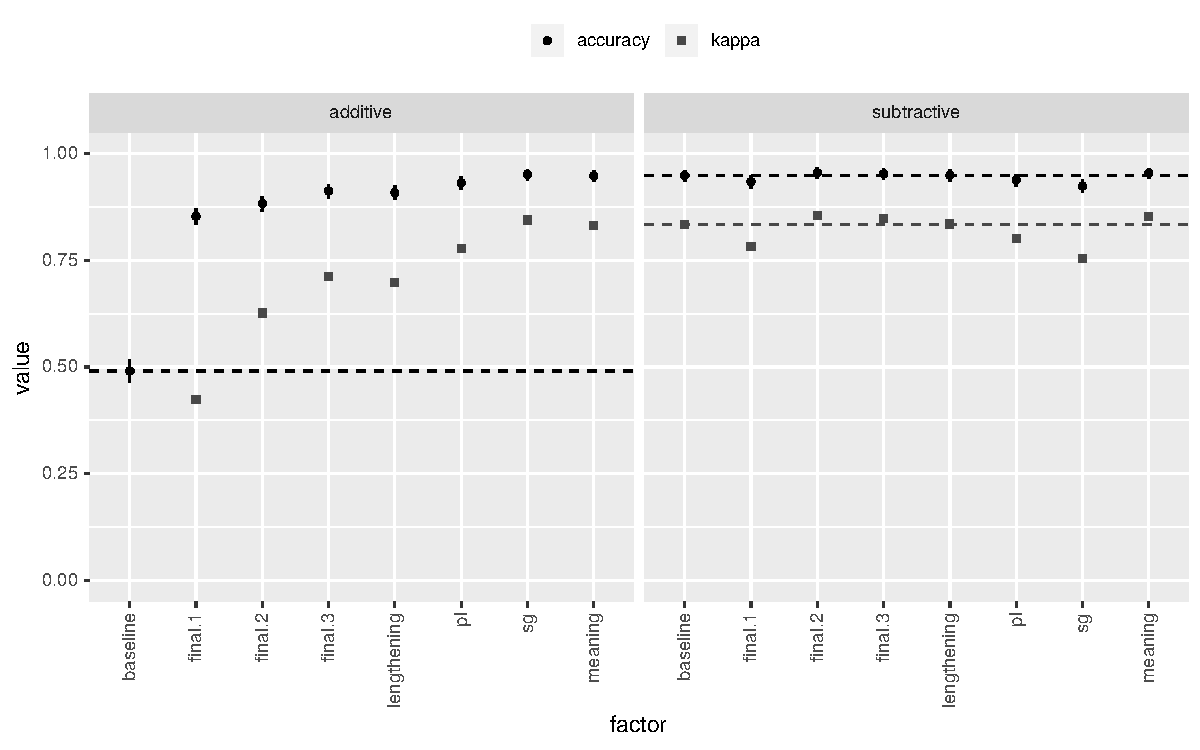
\includegraphics[width=0.9\textwidth]{./figures/kasem/p-fi-dp-sg-overall.pdf}
  \caption{Additive (left) and subtractive (right) accuracy and kappa scores for for the model predicting diphthongization with segmental number markers in Kasem}\label{fig:overall-fi-dp}
\end{figure}

\subsubsection{Predicting lengthening}\label{subsec:pred-length}

The second feature in degree of complexity is the lengthening (or mora insertion) in the plural. In this case we are dealing with a three way choice: no lengthening (NC), consonant lengthening (CC) and vowel lengthening (VV). The best model (not including segmental number markers) was: \texttt{lengthening $\sim$ final.1 + final.2 + final.3}. The results of this model can be seen in \tabref{tab:length-kasem-1} and the corresponding statistics in \tabref{tab:length-kasem-1-stats}.

\begin{table}[t]
  \centering
  \begin{tabular}{lrrr}
    \lsptoprule
    &          Reference\\
    \midrule
    Prediction  &CC  &NL  &VV\\
    CC  &49  &35   &5\\
    NL  &58 &979 &137\\
    VV  &18 &100 &411\\
    \lspbottomrule
  \end{tabular}
    \caption{Confusion matrix for the model predicting lengthening without segmental number markers in Kasem}
  \label{tab:length-kasem-1}
\end{table}

\begin{table}[p]
  \centering\small
  \begin{tabular}{rlll}
    \lsptoprule
    \multicolumn{4}{c}{Overall Statistics}                \\
    \midrule
    \multicolumn{4}{c}{Accuracy : 0.803}                  \\
    \multicolumn{4}{c}{95\% CI : (0.7838, 0.8212)}        \\
    \multicolumn{4}{c}{No Information Rate : 0.6217}      \\
    \multicolumn{4}{c}{Kappa : 0.6046}                    \\
    \midrule
    \multicolumn{4}{c}{Statistics by Class:}              \\
    \midrule
                      & Class: CC & Class: NL & Class: VV \\
    Sensitivity       & 0.392     & 0.879     & 0.743     \\
    Specificity       & 0.976     & 0.712     & 0.905     \\
    Neg Pred Value    & 0.955     & 0.782     & 0.888     \\
    Balanced Accuracy & 0.684     & 0.796     & 0.824     \\
    \lspbottomrule
  \end{tabular}
  \caption{Accuracy scores for \tabref{tab:length-kasem-1}}\label{tab:length-kasem-1-stats}
\end{table}

This model is, once more, already quite good. The type of lengthening a stem undergoes is highly predictable from its shape alone. In this case the semantics did not play any role. Next, we fit a model that includes all other number classes as predictors \texttt{lengthening $\sim$ final.1 + final.2 + final.3 + diphthong + pl + sg}. Results for this model can be seen in \tabref{tab:length-kasem-2} and the corresponding statistics in \tabref{tab:length-kasem-2-stats}.

\begin{table}[p]
  \centering\small
  \begin{tabular}{lrrr}
    \lsptoprule
               & Reference        \\
    \midrule
    Prediction & CC  & NL   & VV  \\
    CC         & 103 & 7    & 11  \\
    NL         & 4   & 1076 & 33  \\
    VV         & 18  & 31   & 509 \\
    \lspbottomrule
  \end{tabular}
    \caption{Confusion matrix for the model predicting lengthening without segmental number markers in Kasem}
  \label{tab:length-kasem-2}
\end{table}

\begin{table}[p]
  \centering\small
  \begin{tabular}{rlll}
    \lsptoprule
    \multicolumn{4}{c}{Overall Statistics}           \\
    \midrule
    \multicolumn{4}{c}{Accuracy : 0.942}             \\
    \multicolumn{4}{c}{95\% CI : (0.9301, 0.9523)}   \\
    \multicolumn{4}{c}{No Information Rate : 0.6217} \\
    \multicolumn{4}{c}{Kappa : 0.8869}               \\
    \midrule
    \multicolumn{4}{c}{Statistics by Class:}         \\
    \midrule

                      & Class: CC & Class: NL & Class: VV \\
    Sensitivity       & 0.824     & 0.966     & 0.920     \\
    Specificity       & 0.989     & 0.945     & 0.961     \\
    Neg Pred Value    & 0.987     & 0.944     & 0.964     \\
    Balanced Accuracy & 0.907     & 0.956     & 0.940     \\
    \lspbottomrule
  \end{tabular}
    \caption{Accuracy scores for \tabref{tab:length-kasem-2}}\label{tab:length-kasem-2-stats}
\end{table}

%\clearpage 
The overall evaluation is shown in \figref{fig:overall-fi-length}. This table presents a more dramatic increase in both kappa and accuracy after adding the segmental number markers. In this case both the singular and plural segmental markers had a very similar importance. More interesting, however, is the fact that in this case we see the opposite effect in the final three segments of the stem. In the previous case of predicting diphthongization, only the final segment was independently predictive of the outcome, here the penultimate and antepenultimate segments are both independently predictive of the lengthening. This again goes to show that different subtrees in the hierarchy have their own analogical relations for their members. Finally, it is worth noting that when predicting diphthongization there was no effect from adding \texttt{lengthening} as a predictor, and here there is no effect from adding \texttt{diphthong} as a predictor. What this suggests is that the correlations described before are already being captured by the final segments. This is the first indication that there is heavy redundancy in the system. I will come back to this in the following sections.

\begin{figure}
  \centering
  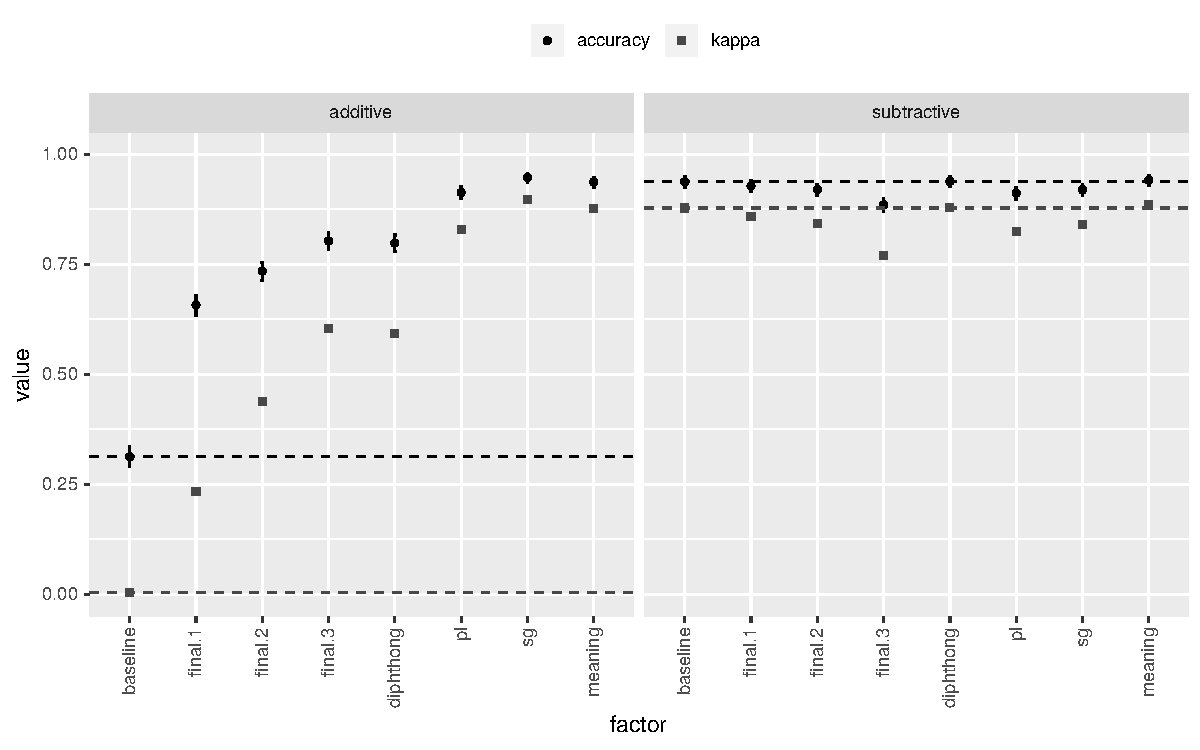
\includegraphics[width=0.9\textwidth]{./figures/kasem/p-fi-length-sg-overall.pdf}
  \caption{Additive (left) and subtractive (right) accuracy and kappa scores for for the model predicting diphthongization with segmental number markers in Kasem}\label{fig:overall-fi-length}
\end{figure}

\subsubsection{Predicting singular markers}

We now turn to predicting the singular marker of a word. 
Because I will be discussing many different models of related phenomena it would be tedious to present confusion matrices or heat maps for each of them. For this reason, I will only present the basic accuracy measures for model comparison. In the last section I will present the heat maps of the final models.

In the first model we are looking at the bare effects of the final segments and meaning of the stems: \texttt{singular $\sim$ final.1 + final.2 + final.3 + meaning}. This model tries to predict total of 14 different markers: \textit{e}, \textit{iə}, \textit{i}, \textit{u}, \textit{ə}, \textit{o}, \textit{gu}, \textit{ŋo}, \textit{m}, \textit{nə}, \textit{go}, \textit{gə}, \textit{ŋə}, \textit{ŋu}. The accuracy scores are shown in \tabref{tab:sg-marker-stem}.

\begin{table}
  \centering
  \begin{tabular}{rl}
    \lsptoprule
    \multicolumn{2}{c}{Overall Statistics}   \\
    \midrule
    Accuracy :            & 0.5709           \\
    95\% CI :             & (0.5476, 0.5939) \\
    No Information Rate : & 0.2037           \\
    Kappa :               & 0.5003           \\
    \lspbottomrule
  \end{tabular}
  \caption{Accuracy scores for the model predicting the singular marker from the stem information only}\label{tab:sg-marker-stem}
\end{table}

This model shows very good performance, especially considering the relatively large number of classes it is predicting. This works as the initial baseline of comparison. The next step is to include the plural marker as a predictor: \texttt{singular $\sim$ final.1 + final.2 + final.3 + meaning + pl}\footnote{The reason for not using the plural stem in these cases is that the plural stem follows directly from knowing the singular stem plus the dimensions of diphthongization and lengthening.}. The accuracy scores are in \tabref{tab:sg-marker-stempl}.

\begin{table}
  \centering
  \begin{tabular}{rl}
    \lsptoprule
    \multicolumn{2}{c}{Overall Statistics} \\
    \midrule
    Accuracy :            & 0.8186         \\
    95\% CI :             & (0.8, 0.8362)  \\
    No Information Rate : & 0.2037         \\
    Kappa :               & 0.7889         \\
    \lspbottomrule
  \end{tabular}
  \caption{Accuracy scores for the model predicting the singular marker from the stem and plural marker information}\label{tab:sg-marker-stempl}
\end{table}

The results in \tabref{tab:sg-marker-stempl} show that there is a considerable gain from including the plural marker in the model. For comparison, using only the plural marker: \texttt{singular $\sim$ pl} produces the results in \tabref{tab:sg-marker-pl}.

\begin{table}
  \centering
  \begin{tabular}{rl}
    \lsptoprule
    \multicolumn{2}{c}{Overall Statistics}   \\
    \midrule
    Accuracy :            & 0.6077           \\
    95\% CI :             & (0.5847, 0.6304) \\
    No Information Rate : & 0.2037           \\
    Kappa :               & 0.5348           \\
    \lspbottomrule
  \end{tabular}
  \caption{Accuracy scores for the model predicting the singular marker from the plural marker information only}\label{tab:sg-marker-pl}
\end{table}

It should then be clear that although the effect of knowing the plural marker is considerable, it is even better when the model knows the shape of the singular stem. The overall results are shown in \figref{fig:overall-fi-singular-sg}, and the heat map for the model using only stem information is in \figref{fig:cm-singular}.

\begin{figure}
  \centering
  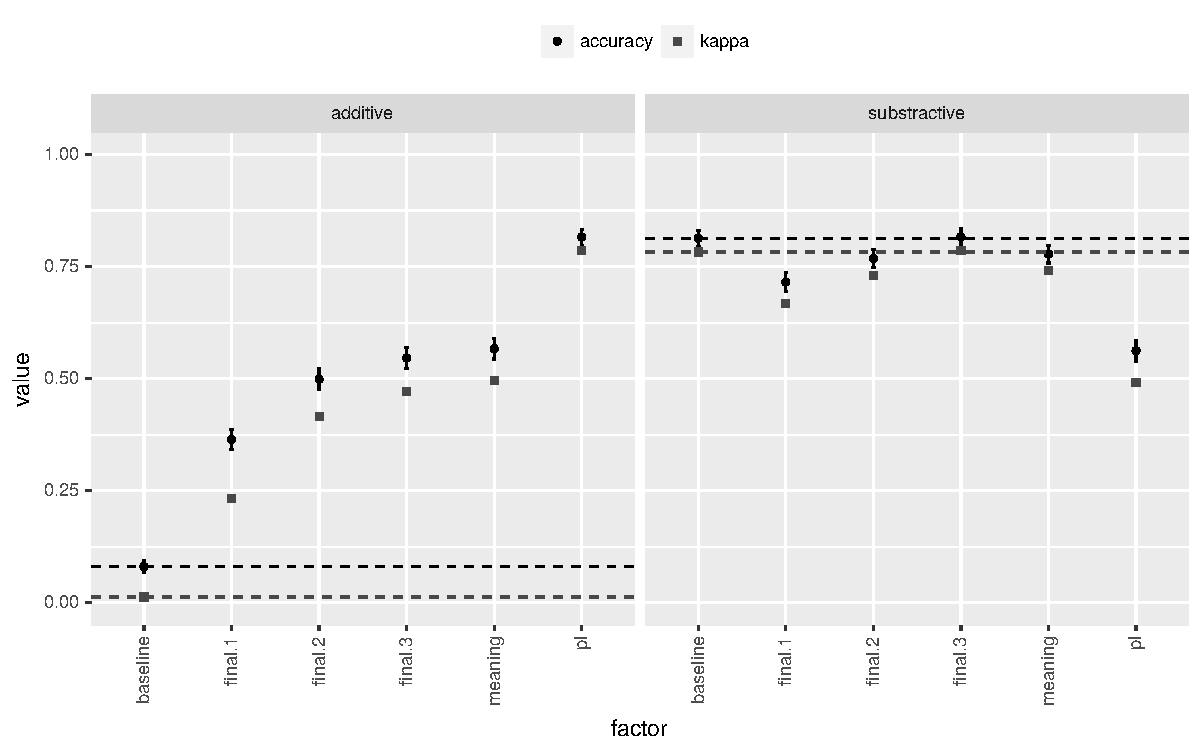
\includegraphics[width=0.9\textwidth]{./figures/kasem/p-fi-sgmark-sg-overall.pdf}
  \caption{Additive (left) and subtractive (right) accuracy and kappa scores for for the model predicting \texttt{singular} from the singular from the stem and plural information}\label{fig:overall-fi-singular-sg}
\end{figure}

\begin{figure}
  \centering
  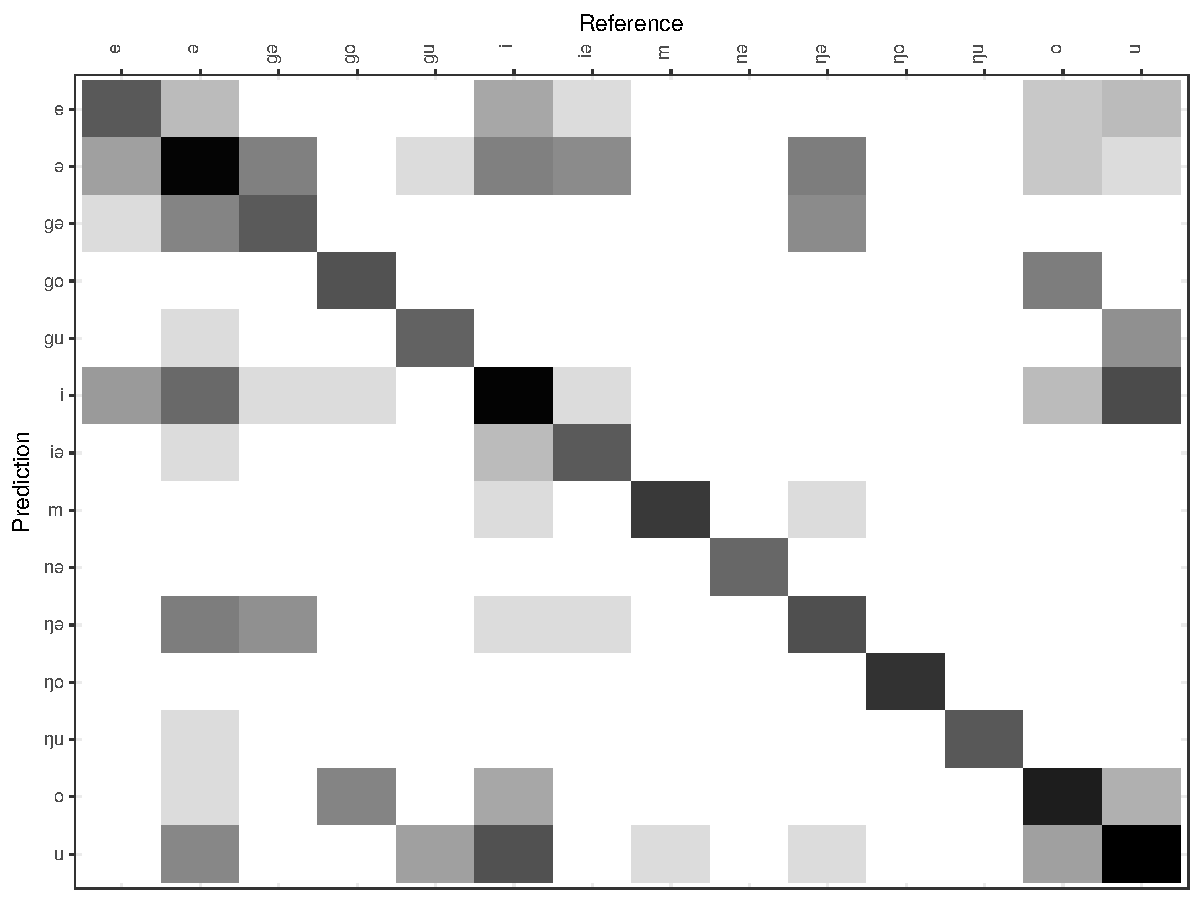
\includegraphics[width=0.9\textwidth]{./figures/kasem/p-singular-sg-cm.pdf}
  \caption{Heat map for the models predicting the singular marker from the stem information only}\label{fig:cm-singular}
\end{figure}


\subsubsection{Predicting plural markers}

We now try to predict the plural marker of a noun. In this case the predicted classes are:  \textit{ə}, \textit{i}, \textit{ru}, \textit{u}, \textit{iə}, \textit{nu}, \textit{e}, \textit{nə}, \textit{m}, \textit{0}, \textit{si}, \textit{en}, \textit{iinə}, \textit{in}.  We first look at the basic model with only the final segments and meaning of the stem: \texttt{plural $\sim$ final.1 + final.2 + final.3 + meaning}. The accuracy results are in \tabref{tab:pl-marker-stem}.

\begin{table}[t]
  \centering
  \begin{tabular}{rl}
    \lsptoprule
    \multicolumn{2}{c}{Overall Statistics}   \\
    \midrule
    Accuracy :            & 0.6345           \\
    95\% CI :             & (0.6117, 0.6568) \\
    No Information Rate : & 0.3265           \\
    Kappa :               & 0.5528           \\
    \lspbottomrule
  \end{tabular}
  \caption{Accuracy scores for the model predicting the plural marker from the stem information only}\label{tab:pl-marker-stem}
\end{table}

Next, we test the effect of adding the singular marker: \texttt{plural $\sim$ final.1 + final.2 + final.3 + meaning + sg}. The results of this model are in \tabref{tab:pl-marker-sgstem}.

\begin{table}
  \centering
  \begin{tabular}{rl}
    \lsptoprule
    \multicolumn{2}{c}{Overall Statistics}  \\
    \midrule
    Accuracy :            & 0.8867          \\
    95\% CI :             & (0.8711, 0.901) \\
    No Information Rate : & 0.3265          \\
    Kappa :               & 0.8615          \\
    \lspbottomrule
  \end{tabular}
  \caption{Accuracy scores for the model predicting the plural marker from the stem and singular marker}\label{tab:pl-marker-sgstem}
\end{table}

\tabref{tab:pl-marker-sgstem} shows that the plural marker is more predictable than the singular marker. A possible simple explanation is that it is more common that one would want to predict the plural of a noun from knowing its singular form, than wanting to predict the singular form of a noun from knowing its plural. A very similar situation arises if we try to predict the plural marker from the singular marker alone: \texttt{plural $\sim$ sg}. The results are in \tabref{tab:pl-marker-sg}.

\begin{table}
  \centering
  \begin{tabular}{rl}
    \lsptoprule
    \multicolumn{2}{c}{Overall Statistics}  \\
    \midrule
    Accuracy :            & 0.7204          \\
    95\% CI :             & (0.699, 0.7411) \\
    No Information Rate : & 0.3265          \\
    Kappa :               & 0.6468          \\
    \lspbottomrule
  \end{tabular}
  \caption{Accuracy scores for the model predicting the plural marker from the singular marker information only}\label{tab:pl-marker-sg}
\end{table}

These results show a greater symmetry in the implicational relations. The overall results and evaluation can be seen in \figref{fig:overall-fi-plural-sg}, and the heat map for the model using only the stem is in \figref{fig:cm-plural}.

\begin{figure}
  \centering
  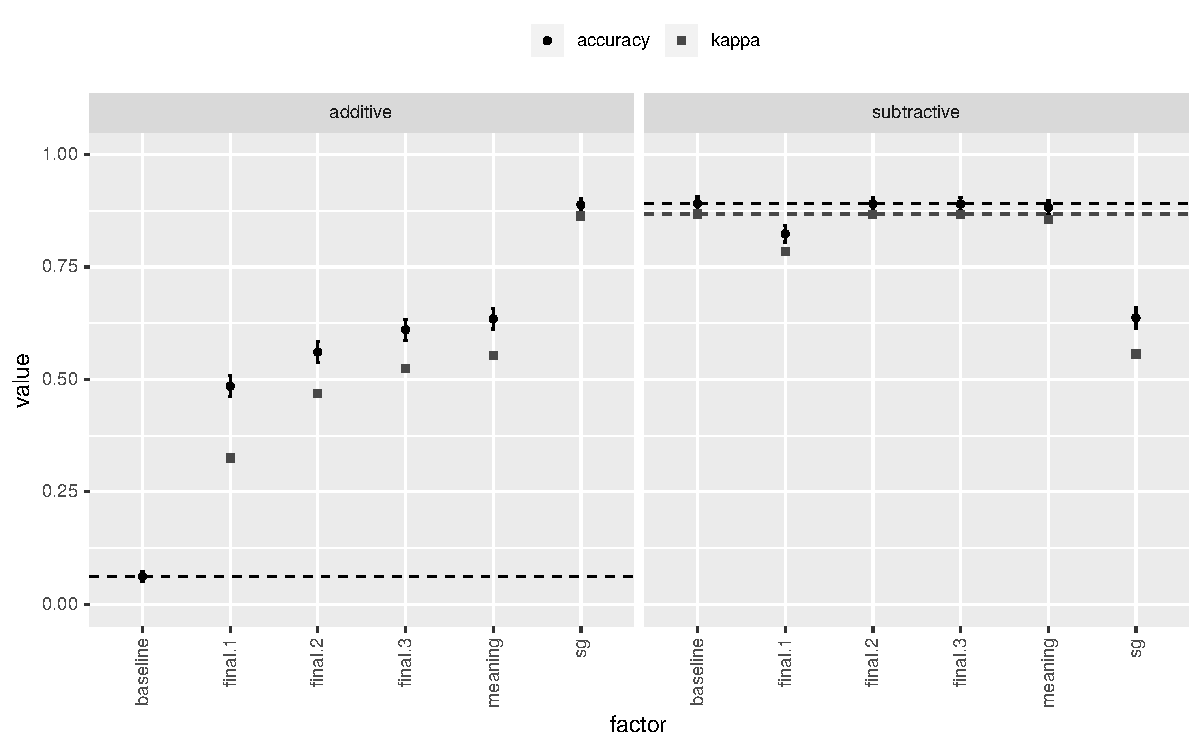
\includegraphics[width=0.9\textwidth]{./figures/kasem/p-fi-plmark-sg-overall.pdf}
  \caption{Additive (left) and subtractive (right) accuracy and kappa scores for for the model predicting \texttt{plural} from the singular stem in Kasem}\label{fig:overall-fi-plural-sg}
\end{figure}

\begin{figure}
  \centering
  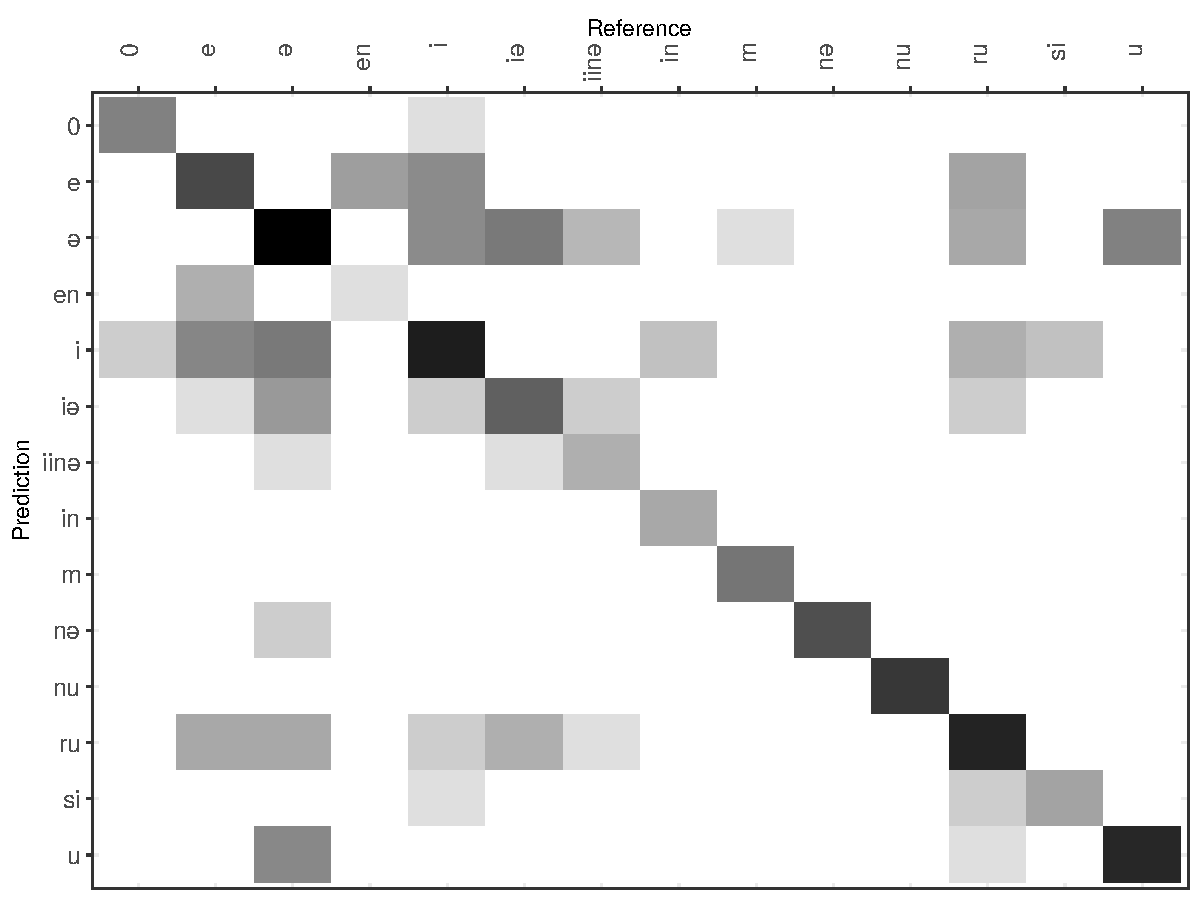
\includegraphics[width=0.9\textwidth]{./figures/kasem/p-plural-sg-cm.pdf}
  \caption{Heat map for the models predicting the plural marker from the stem information only}\label{fig:cm-plural}
\end{figure}


\subsubsection{Predicting class}

Finally, we want to put these things together and predict inflectional class (defined as the combination of a singular and a plural marker). So far I did not include diphthongization and lengthening as part of the inflectional class. Doing so would result in too many labels, which the model would have a very hard time predicting. Additionally, as seen when predicting diphthongization and lengthening, both these sub-trees are fairly predictable from the same factors\footnote{This has the additional problem that it burdens the analogical model, since the factors will be doing multiple jobs at the same time.}. I will instead use both factors (diphthongization and lengthening) as predictors of class. As before, there is no real limit to possible combinations of factors and classes one can test.

First we predict from the stem with a basic model that only looks at the ending and meaning of the stem: \texttt{class $\sim$ final.1 + final.2 + final.3 + meaning}. The results are in \tabref{tab:class-marker-stem} and its corresponding heat map in \figref{fig:cm-class-stem}

\begin{table}
  \centering
  \begin{tabular}{rl}
    \lsptoprule
    \multicolumn{2}{c}{Overall Statistics}  \\
    \midrule
    Accuracy :& 0.5335\\
    95\% CI :& (0.5101, 0.5568)\\
    No Information Rate :& 0.1791\\
    Kappa :& 0.4928\\
    \lspbottomrule
  \end{tabular}
  \caption{Accuracy scores for the model predicting inflection class from the stem only}\label{tab:class-marker-stem}
\end{table}

\begin{figure}
  \centering
  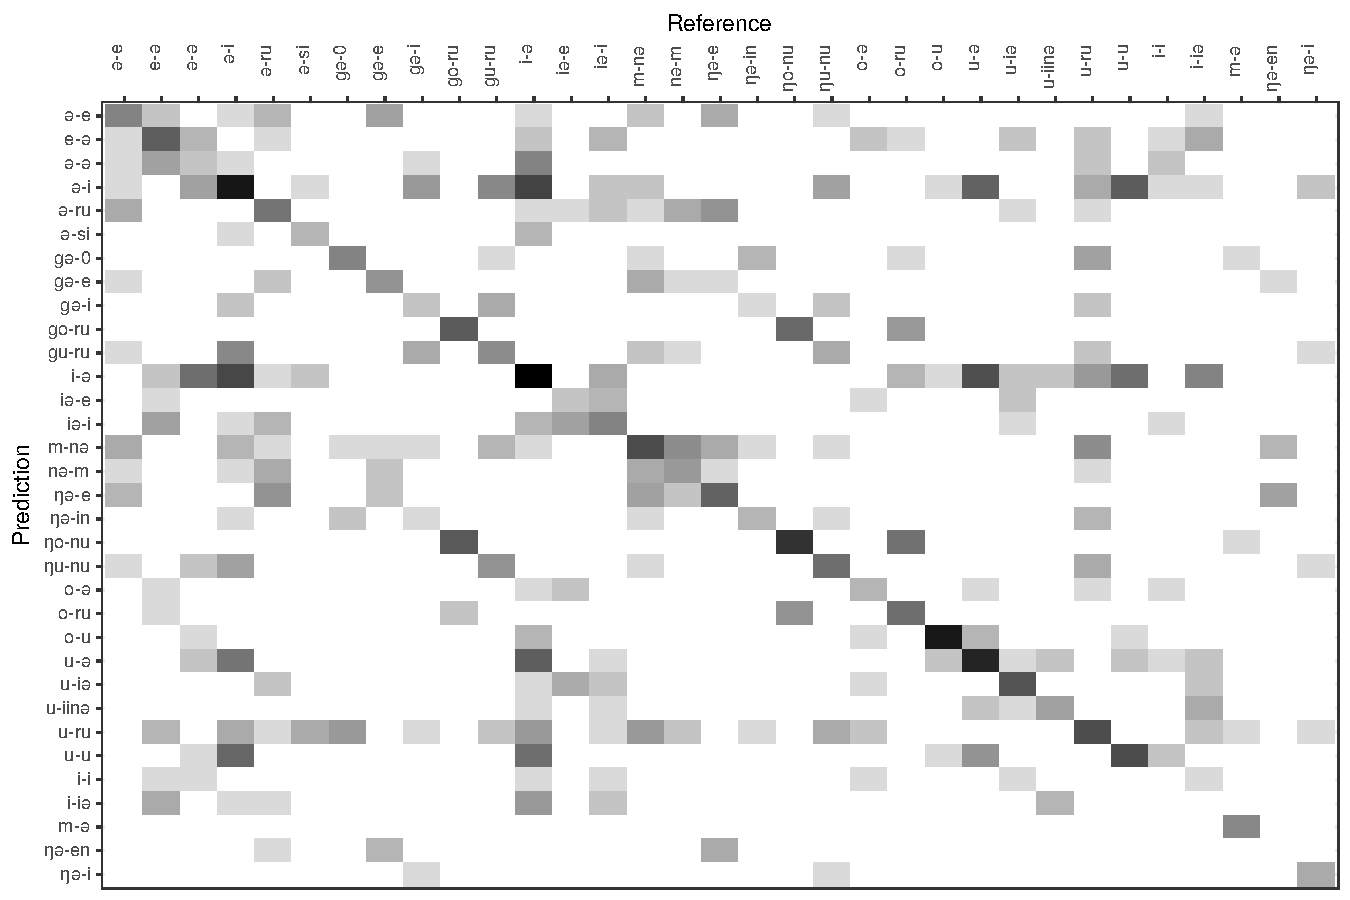
\includegraphics[width=0.9\textwidth]{./figures/kasem/p-class-sg-cm.pdf}
  \caption{Heat maps for the models predicting inflection from the stem only}\label{fig:cm-class-stem}
\end{figure}

Including \texttt{lengthening} and \texttt{diphthong} as predictors with the formula: \texttt{class $\sim$ final.1 + final.2 + final.3 + lengthening + diphthong + meaning}, produces a clear improvement. The results can be seen in \tabref{tab:class-marker-dplengthstem}, the corresponding heat map can be seen in \figref{fig:cm-class-sg-2}, and the overall evaluation in \figref{fig:overall-fi-class-sg}.

\begin{table}
  \centering
  \begin{tabular}{rl}
    \lsptoprule
    \multicolumn{2}{c}{Overall Statistics}  \\
    \midrule
    Accuracy :& 0.6596\\
    95\% CI :& (0.6371, 0.6815)\\
    No Information Rate :& 0.1791\\
    Kappa :& 0.6303\\
    \lspbottomrule
  \end{tabular}
  \caption{Accuracy scores for the model predicting the plural marker from the singular marker information only}\label{tab:class-marker-dplengthstem}
\end{table}

\begin{figure}
  \centering
  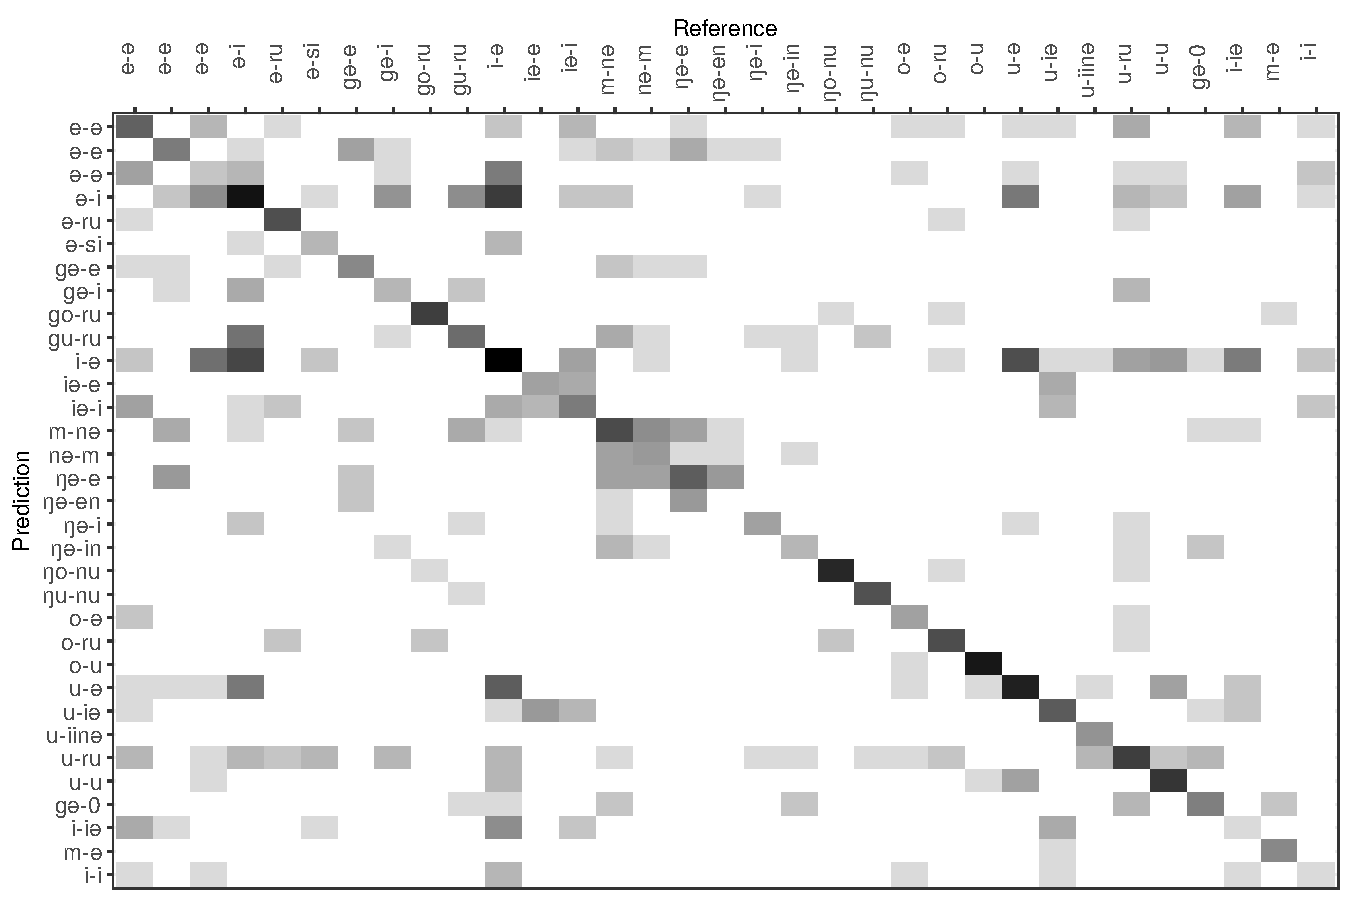
\includegraphics[width=0.9\textwidth]{./figures/kasem/p-class-sg-cm-2.pdf}
  \caption{Heat maps for the models predicting inflection class from the stem, and lengthening and diphthongization information}\label{fig:cm-class-sg-2}
\end{figure}

\begin{figure}
  \centering
  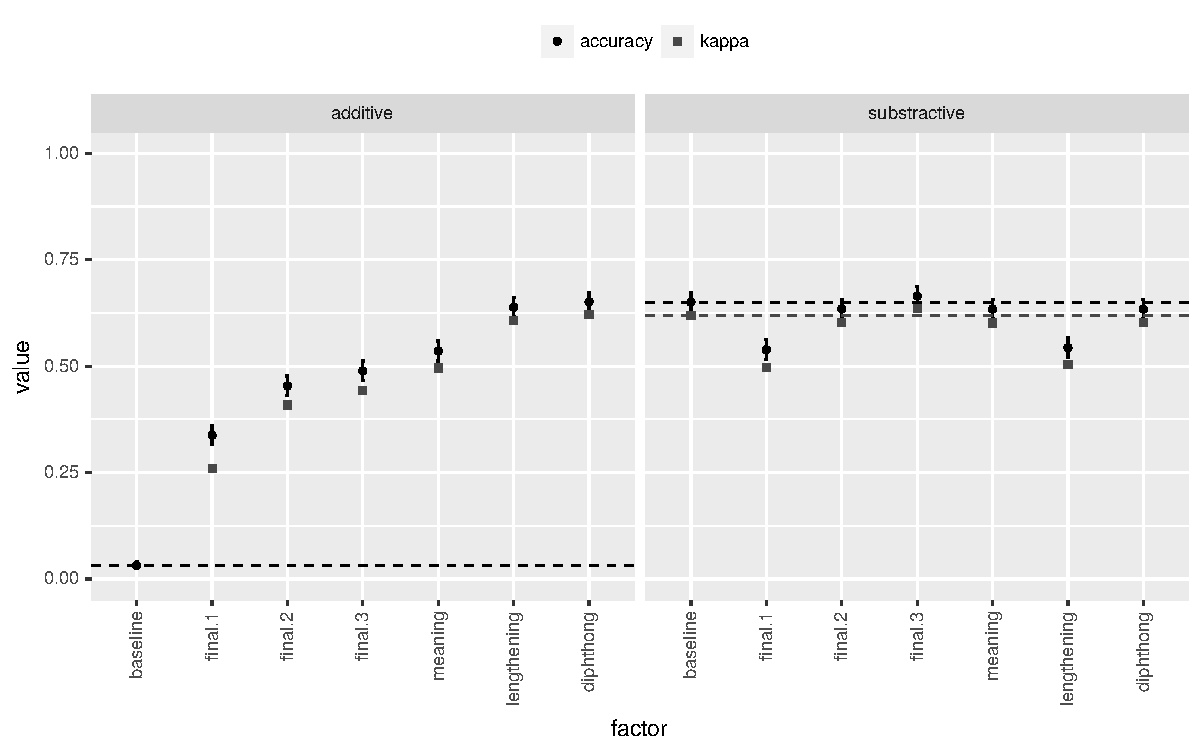
\includegraphics[width=0.9\textwidth]{./figures/kasem/p-fi-class-sg-overall.pdf}
    \caption{Additive (left) and subtractive (right) accuracy and kappa scores for for the model predicting inflection class}\label{fig:overall-fi-class-sg}
\end{figure}

In this case it is also useful to look at the balanced by-class accuracy of the model. That is, we can look at how each level of the response variable (each inflectional class) increases or decreases in accuracy as we add or subtract factors. These results are shown in \figref{fig:byclass-fi-class-sg}. The interesting point here is that different classes are not equally predictable. What this means is that there is not an homogeneous increase in the class accuracy. Instead, some classes like \textit{o-u} or \textit{e-ə} achieve a very high balanced accuracy with the use of just one predictor, while classes like \textit{ə-ə} and \textit{iə-e} remain quite unpredictable all the way through. This indicates that class predictability is not symmetric, and that different classes focus on different parts of the stem.

\begin{sidewaysfigure}
  \centering
  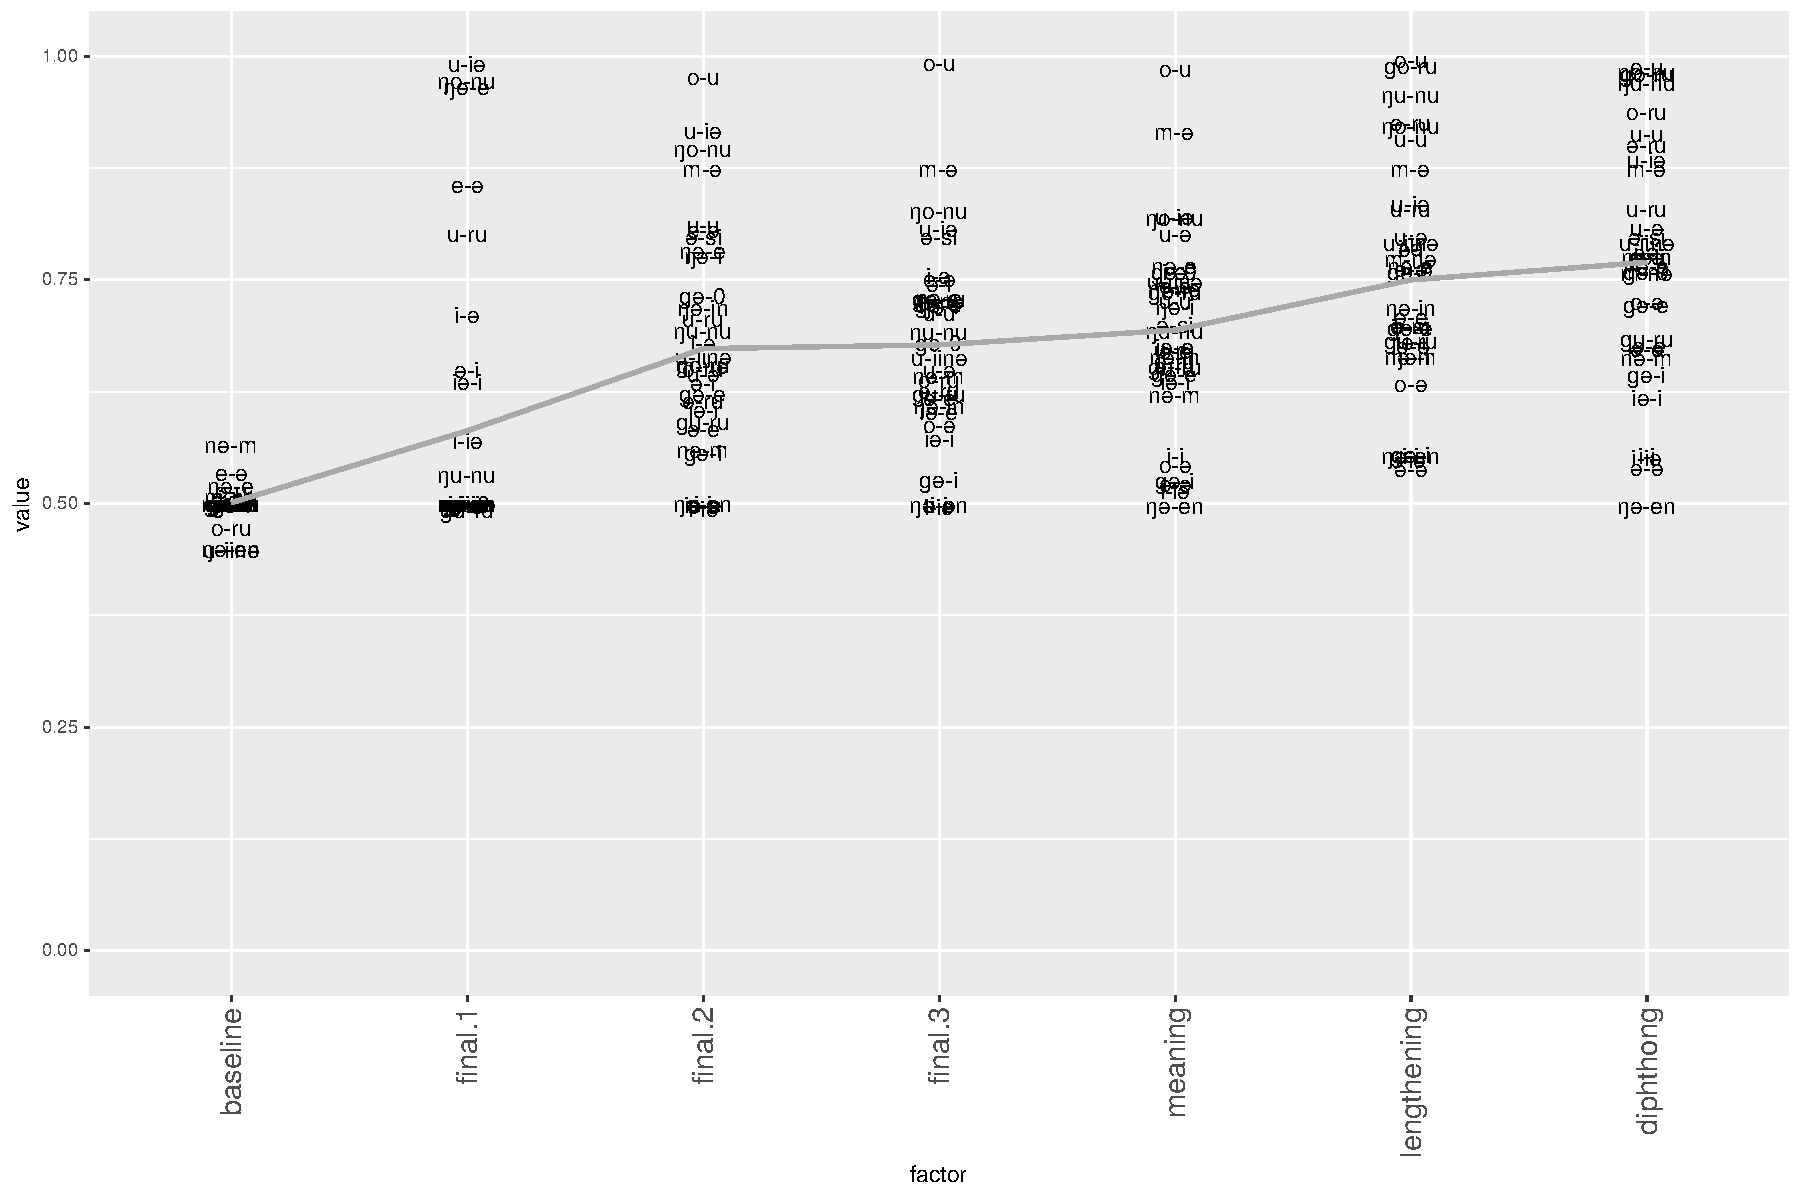
\includegraphics[width=0.85\textheight]{./figures/kasem/p-fi-class-sg-byclass.pdf}
  \caption{Additive balanced accuracy (by class) for the model predicting inflection class}\label{fig:byclass-fi-class-sg}
\end{sidewaysfigure}

Finally, the clustering created by this model\footnote{As before, we fit a direct similarity model instead of relying on the errors of the analogical model.} presents several crucial results. Like in Spanish, this is the most interesting aspect of the models. The first thing we can observe is that the larger (color coded) clusters are not homogenous with respect to the features that seem to define them. There are several important clusters to look at here. On the left top corner, in dark green, we find an inversion \textit{-i/-ə} -- \textit{-ə/-i}, next to \textit{-u/-ə} which fits the general pattern of an \textit{-ə} with a high vowel. To the right, and around the -0.5 X axis, we find three classes: \textit{-ə/-ə}, \textit{-i/-i} and \textit{-u/-u}. The first two are close to each other and clustered together, while the last class is clustered separate from the other two, but it is placed quite close to them on the map.

Close, and tightly grouped together, we find two clusters, one in dark blue and one in light lilac. These two clusters all share an \textit{-iə} marker, except for one which only has a \textit{-ə} marker. In dark blue we see an inversion between \textit{-iə/-i} and \textit{-i/-iə}, and in light lilac a partial inversion of \textit{-iə} marking singular and plural. The next color clusters are less well organized from a perspective of a potential hierarchy, but from their position they make sense. On the lower right corner we see three classes that share an \textit{-o} in the singular and \textit{-u} in the plural, with some additional \textit{-g-}, \textit{-r-} and \textit{-ŋ-}. Right at the 0.5 X and -0.25 Y we find other two classes with a \textit{-ru} marking plural (again, close to the \textit{-o/-ru} and \textit{-go/-ru} classes).

Right at the center of the map we see three classes: \textit{-u/-iinə}, \textit{-m/-ə} and \textit{-ə/-si}. These classes only share the \textit{-ə} marker (or /ə/ segment in the case of \textit{-innə}), but they have in common that they have one marker not shared by any other class. At the same X coordinate, but at around 0.5 Y, we have two close classes having a \textit{-[+velar]ə} marker for the singular and \textit{-i} in the plural, and not too far off we have the very similar \textit{-ŋə/-in} class (arguably the class \textit{-gə/-$\emptyset$} is also related to these three classes). A class that seems somewhat out of place is the \textit{-gu/-ru} class, also in dark orange. Finally, in the top right corner we have two groups. In light blue we have classes with \textit{-ə/-e} plus additional markers, and in dark lilac we have the inversion \textit{-nə/-m} -- \textit{-m/-nə}.

A second important result that can be observe in this clustering is that the presence or absence of \textit{ŋ}, \textit{n}, \textit{r}, \textit{s} and \textit{m} markers is not random on the map. All these markers only appear with positive values on the X axis. Similarly, most velar markers are in the upper right quadrant. What this indicates is that these markers cluster independently of the vocalic markers, lending some evidence to the hypothesis that each subtree in the hierarchy has its own analogical function.

Important for the sketch of the system presented above is that for most classes their position on the plane depends more on the vowel presence or combinations, than on what they mark. That is, \textit{-x/-y} classes are close to other classes with either \textit{-x} or \textit{-y} present, independently of whether \textit{-x} and \textit{-y} are marking the same number. This is exactly what the hierarchy suggested would predict.

\begin{sidewaysfigure}
  \centering
  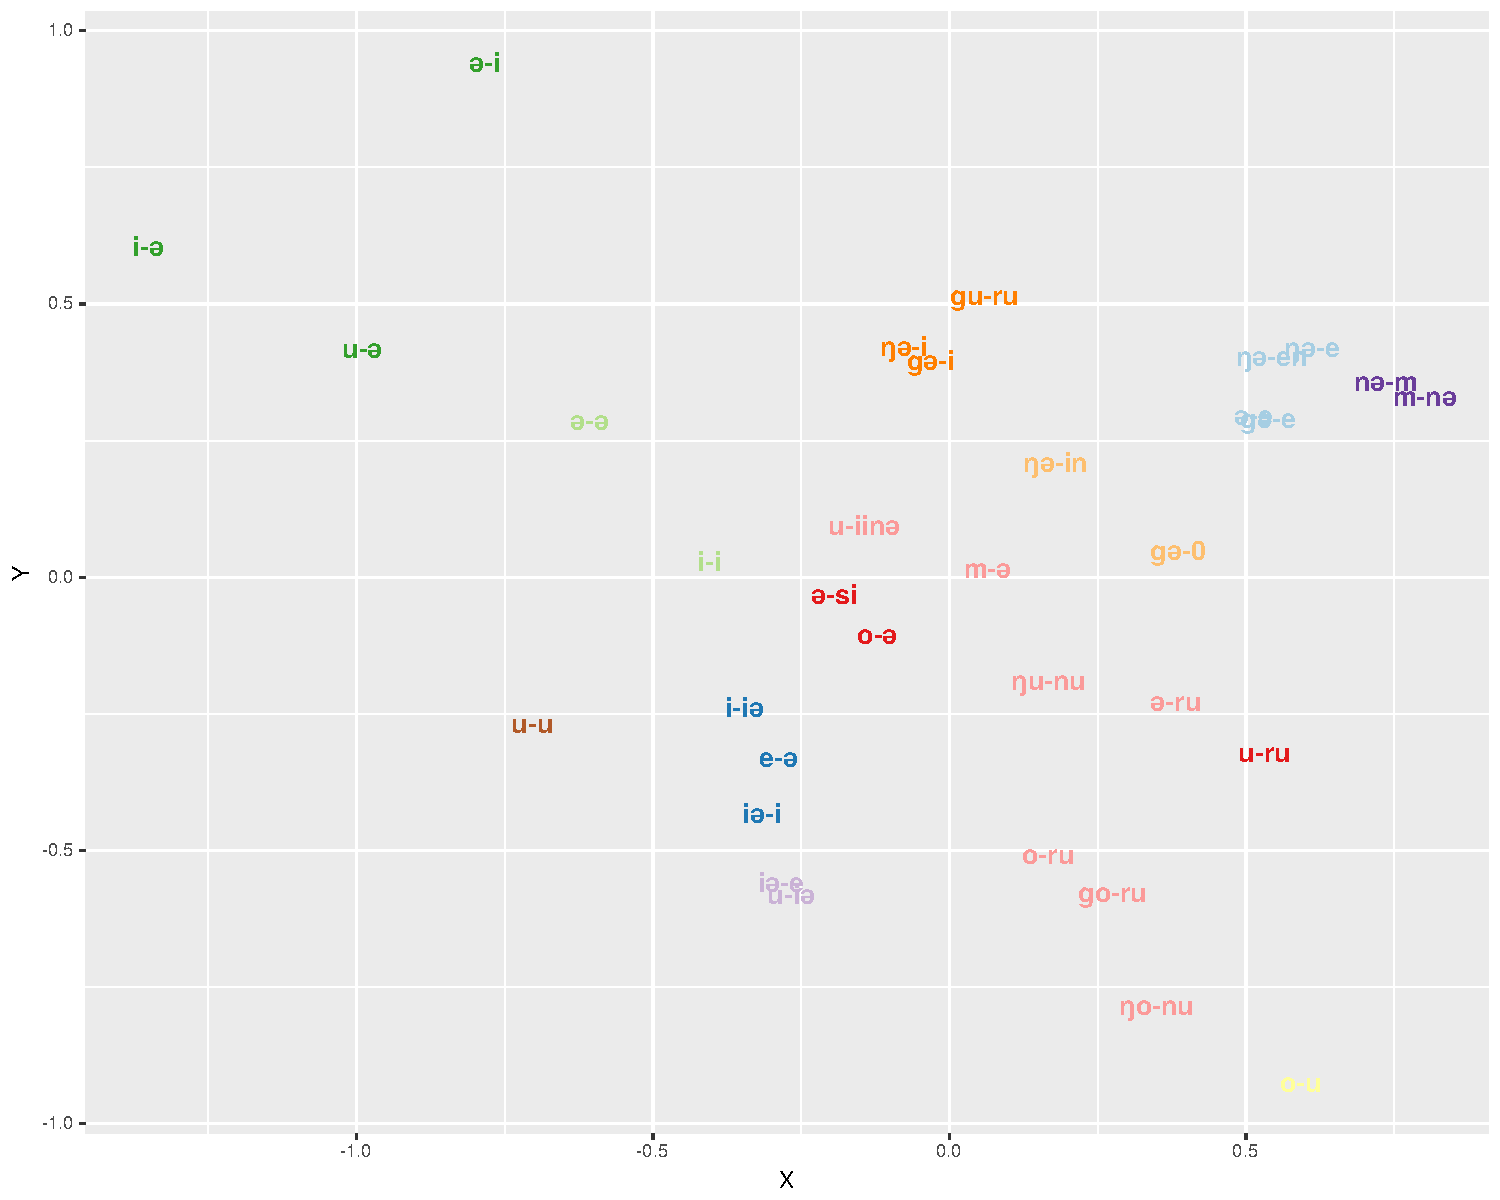
\includegraphics[width=0.7\textwidth]{./figures/kasem/kasem-nouns-hclust-sim-sg-pred.pdf}
  \caption{Clustering of inflection class in Kasem based on the singular stem, lengthening and diphthongization}\label{fig:class-cluster-kasem}
\end{sidewaysfigure}

Finally, because of the complexity of the system, we can test whether there are extra similarity dimensions we are missing in this MDS plot. To do this, we extract three main components of the similarity matrix instead of two, and plot them side by side. This is similar to looking at a cube from three of its faces. In the plots in \figref{fig:class-cluster-kasem-3}, X is the first component, Y the second and Z the third.

The XY plot shows the same map as before for comparison. The most interesting effect is found in the ZY plot. Here a strong grouping of the classes across vocalic lines appears. Classes with /o/ and /u/ are mostly on the lower quadrants, and classes with /ə/ and /i/ tend to be higher. Particularly interesting is the repositioning of \textit{-ə/-i} to the right quadrant, closer to other classes with the same sequence of vocalic markers. The XZ plot is less interesting, but it shows a much stronger separation of the purely vocalic class from classes with multiple exponents. Although the evidence is somewhat weaker, we see that different similarity dimensions capture what seems to be different aspects of the hierarchy.

What this decomposition shows is that the grouping effects between the classes go beyond two dimensions. That is, our two dimensional representation of class similarity can only capture a portion of the relevant information. This makes sense from a cross-classification perspective. Two classes might be similar to each other along some dimension, but different from each other along some other dimension. The MDS diagrams are only approximations of the actual similarity effects between classes.

\begin{sidewaysfigure}
  \centering
  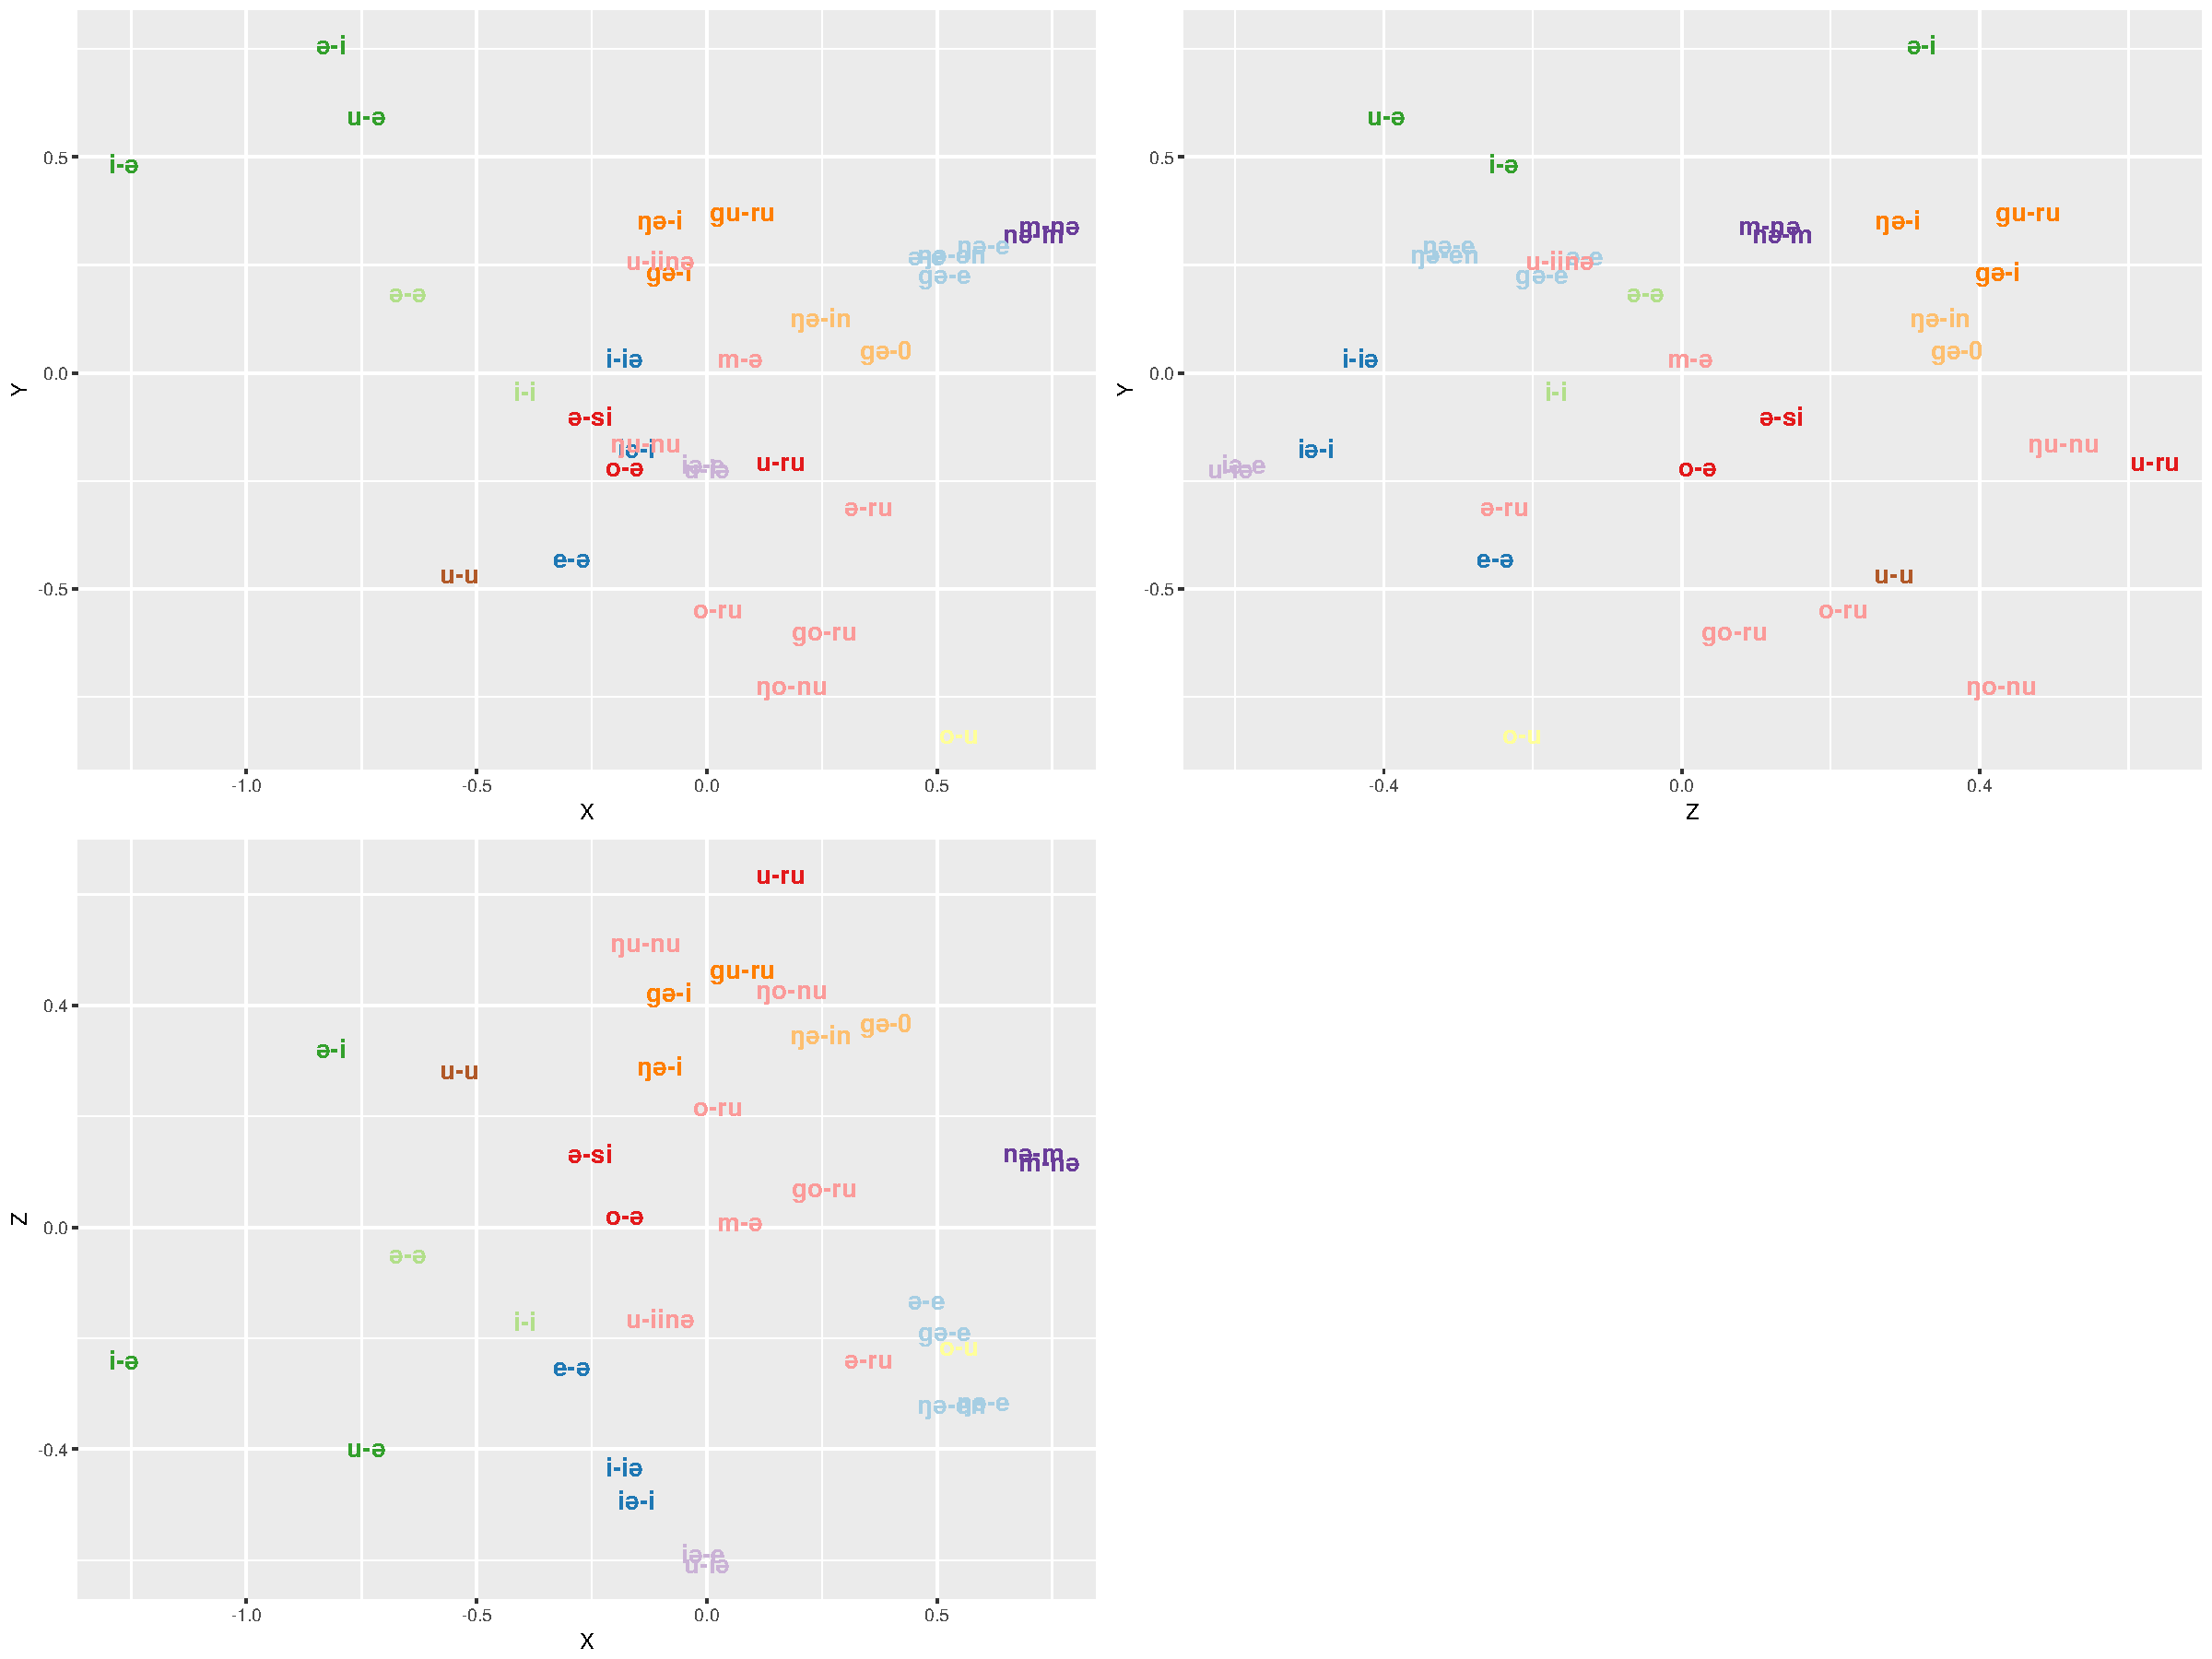
\includegraphics[width=0.7\textwidth]{./figures/kasem/kasem-nouns-hclust-sim-multi.pdf}
  \caption{Clustering of inflection class in Kasem based on the singular stem, lengthening and diphthongization across multiple dimensions}\label{fig:class-cluster-kasem-3}
\end{sidewaysfigure}

\section{Interim Conclusion}

In this chapter I looked at two complex inflectional systems: Spanish verb inflection and Kasem singular-plural classes. In Spanish, verbs are divided into three main inflection classes: \textit{-ar}, \textit{-er} and \textit{-ir} verbs. Additionally, a set of verbs show different kinds of vocalic and consonant stem alternations in the present tense and past participle. Analogical models trained on the phonological shape of the stems could predict with high accuracy the main inflection class of verbs, and the stem alternation that verbs exhibit. The clustering based on stem similarity showed that verbs that undergo the same stem alternation have similar stems, even if they belong to different main inflection classes.

I propose that these facts taken together constitute very strong evidence that the analogical relations do not only choose one of the trees in the hierarchy, but go up all of them. Naturally, this does not mean that we should always see perfect correlations, but rather that the correlations between the analogical relations and the grammatical hierarchy will be present.

In Kasem, nouns can take a variety of different singular and plural markers. A key feature of this system is that individual markers can denote singular and plural in different nouns. In addition to this, nouns can undergo diphthongization and vowel lengthening in the plural. These three dimensions (markers, lengthening and diphthongization) produce the inflection class of nouns. The analogical models, trained on the phonological shape and meaning of the stems, could correctly distinguish these three dimensions, and predict with a high degree of accuracy the inflection class of nouns. The models showed that inflection class is almost equally predictable from the stem as it is from the singular or plural marker alone.

\newpage 
The clustering analysis in Kasem showed that inflection classes that shared the same markers clustered together, even if markers were flipped, i.e. marking singular in one class and plural in the other class. This means that the analogical relations must also hold at a more abstract level, and not just on the leaves of the hierarchy. This is because if nouns of classes \textit{ә--i} and \textit{u--ә} (as many other cases discussed above) are similar to each other, it means that at some level both classes must share a general type \textit{ә} underspecified for number.

Overall, this chapter shows that the kind of analogical classifiers proposed in this book can model very complex systems with many classes. It also shows analogical relations still reveal aspects of the hierarchy, even if said hierarchy includes very complex interactions of multiple dimensions. 
%The two case studies in this chapter constitute strong evidence for a model in which analogy runs through the hierarchy.

\il{Kasem|)}
\is{inflection|)}

%%% Local Variables:
%%% mode: latex
%%% TeX-master: "../main"
%%% End:
